\documentclass{article}
\usepackage[utf8x]{inputenc}
\usepackage{graphicx}
\usepackage{tikz, amsmath, amssymb, bm, color}
\usepackage{geometry}
\usetikzlibrary{calc}
\usetikzlibrary{shapes,arrows}
\usepackage{todonotes}
\usepackage[american]{circuitikz}
\usepackage{pgfplots}
\usepackage{epstopdf}
\usepackage{listings}
\usepackage{subcaption}
\usepackage{mwe}
\usepackage{float}
\usepackage{cleveref}
\usepackage{ragged2e} % For text alignment


\newenvironment{custom_itemize}{
\begin{itemize}
  \setlength{\itemsep}{0pt}
  \setlength{\parskip}{0pt}
  \setlength{\parsep}{0pt}
}{\end{itemize}}


%\usepackage{multicol} % Used for the two-column layout of the document


%\usepackage{bm}


\title{Preethi's ROIC analysis}
\author{Kees Kroep 4246373}


\begin{document}
%  \twocolumn[{%
% \begin{@twocolumnfalse}
  \maketitle
%   \end{@twocolumnfalse}
% }]
i
\section{setup}\label{sec:setup}
\begin{figure}[H]
\centering
\usetikzlibrary{shapes,snakes}
\tikzstyle{dot} = [draw,shape=circle,fill=black, scale =.2]
\tikzstyle{l_arrow} = [draw,fill = black, regular polygon,regular polygon sides=3, rotate=-90, anchor=south, scale=.5] 
\tikzstyle{l_text} = [anchor=south west]
\tikzstyle{r_arrow} = [draw,fill = black, regular polygon,regular polygon sides=3, rotate=90, anchor=south, scale=.5] 
\tikzstyle{r_text} = [anchor=south east]
\begin{tikzpicture}[scale=1.5, every node/.style={scale=1}]


\node[l_text] at (-3,1) {VDD 3.3 (1)};
\node[l_text] at (-3,0) {IN[8] (15)};
\node[l_text] at (-3,-1) {VSUB (16)};
\node[l_text] at (-3,-2) {VDD\_HV (17)};
\node[l_text] at (-3,-3) {GND\_HV (18)};

\node[l_arrow] at (-3,1) {};
\node[l_arrow] at (-3,0) {};
\node[l_arrow] at (-3,-1) {};
\node[l_arrow] at (-3,-2) {};
\node[l_arrow] at (-3,-3) {};

\node[r_text] at (0,1) {(25) gnd};
\node[r_text] at (0,0) {(26) VDD5};
\node[r_text] at (0,-1) {(27) Vg};
\node[r_text] at (0,-2) {(28) Rst[3]};
\node[r_text] at (0,-3) {(29) Rst[1]};
\node[r_text] at (0,-4) {(30) Rst[2]};
\node[r_text] at (0,-5) {(31) Res};
\node[r_text] at (0,-6) {(32) VB0[8]};
\node[r_text] at (0,-7) {(33) out[8]};
\node[r_text] at (0,-8) {(48) gnd};


\node[r_arrow] at (0,1) {};
\node[r_arrow] at (0,0) {};
\node[r_arrow] at (0,-1) {};
\node[r_arrow] at (0,-2) {};
\node[r_arrow] at (0,-3) {};
\node[r_arrow] at (0,-4) {};
\node[r_arrow] at (0,-5) {};
\node[r_arrow] at (0,-6) {};
\node[r_arrow] at (0,-7) {};
\node[r_arrow] at (0,-8) {};
\draw  (-3,2) rectangle (0,-8);




\draw (-3.5,-1) node[ground]{} to (-3,-1);
\draw (-3.5,-3) node[ground]{} to (-3,-3);
\draw (0.5,1) node[ground]{} to (0,1);
\draw (0.5,-8) node[ground]{} to (0,-8);
\draw (0.5,-3) node[ground]{} to (0,-3);
\draw (0.5,-4) node[ground]{} to (0,-4);

\draw (0.5,0.25) node[anchor=south]{$5\,V$} (0.5,0.25) node[tground]{} to (0.5,0)to (0,0); % VDD5
\draw (0.5,-0.75) node[anchor=south]{$4.5\,V$} (0.5,-0.75) node[tground]{} to (0.5,-1)to (0,-1); % Vg
\draw (-3.5,1.25) node[anchor=south]{$3.3\,V$} (-3.5,1.25) node[tground]{} to (-3.5,1)to (-3,1); % VDD3.3
\draw (-3.5,-1.75) node[anchor=south]{$5\,V$} (-3.5,-1.75) node[tground]{} to (-3.5,-2)to (-3,-2); %VDD_HV
\draw (-4.5,0.25) node[anchor=south]{$set$} (-4.5,0.25) node[tground]{} to (-4.5,0)to (-4.5,0); % IN[8]
\draw (0.5,-1.75) node[anchor=south]{$reset$} (0.5,-1.75) node[tground]{} to (0.5,-2)to (0,-2); % Rst[3]
\draw  (0,-5) to[R=$50\,k\Omega$](1.5,-5) to (1.5,-4.75) node[tground]{} (1.5,-4.75) node[anchor=south]{$5\,V$}; %res


\draw (-4.5,0) to [R=$20\,M\Omega$](-3,0);

\end{tikzpicture}
\caption{Schematic of breadbord}
\label{tkz:breadbord}
\end{figure}
\begin{figure}[H]
\centering
\usetikzlibrary{shapes,snakes}
\tikzstyle{dot} = [draw,shape=circle,fill=black, scale =.3]
\tikzstyle{l_arrow} = [draw,fill = black, regular polygon,regular polygon sides=3, rotate=-90, anchor=south, scale=.5] 
\tikzstyle{l_text} = [anchor=south west]
\tikzstyle{r_arrow} = [draw,fill = black, regular polygon,regular polygon sides=3, rotate=90, anchor=south, scale=.5] 
\tikzstyle{r_text} = [anchor=south east]
\begin{tikzpicture}[scale=1, every node/.style={scale=1}]

\draw[dashed, color=blue]  (-0.5,5.5) rectangle (0.5,-2);
\fill[color=blue, opacity=.1]  (-0.5,5.5) rectangle (0.5,-2);
\node[align=center, anchor=south] at (0,5.5) {voltage\\limiter};

\draw[dashed, color=green]  (1.25,5.5) rectangle (5.25,-2);
\fill[opacity=.1, color=green]  (1.25,5.5) rectangle (5.25,-2);
\node[align=center, anchor=south] at (3.25,5.5) {integrator};



\draw[dashed, color=red]  (5.75,5.5) rectangle (9.25,-2);
\fill[opacity=.1, color=red] (5.75,5.5) rectangle (9.25,-2);
\node[align=center, anchor=south] at (7.5,5.5) {current mirrors};

%\draw (0,0) to node[nfet]{};

%\draw (0,0) to (mos1.s);
\node(Vg)[nfet, rotate=-90] at (0,2.5) {};
\node[nfet, rotate=-90] (Reset) at (2.5,2) {};
\node[pfet] (CM_H1) at (5,3) {};
\node[nfet] (CM_L1) at (5,-1) {};
\node[nfet] (CM_H2) at (7,3) {};
\node[nfet] (CM_L2) at (7,-1) {};
\node[nfet] (CM_H3) at (9,3) {};
\node[nfet] (CM_L3) at (9,-1) {};



\draw (-1,2.5) node[anchor=east]{IN[i]} to (Vg.S);
\draw (Vg.G) |- (0,4.5) node[anchor=south]{Vg};
\draw (Vg.B) |- (1,2.5) node[dot]{} |- (CM_H1.G); %top
\draw (1,2.5) |- (1,0.5)  to [C=$450\,fF$](4,0.5) -| (CM_H1.D);
\draw (1.5,0.5) node[dot]{} -| (1.5,2) |- (Reset.B);
\draw (Reset.G) to (2.5,4.5) node[anchor=south]{Rst[3]};
\draw (Reset.D) -| (3.5,0.5) node[dot]{};
\draw (5,0.5) node[dot]{} to (CM_L1.D);
\draw (CM_L1.G) to (4,4.5) node[anchor=south]{Res}; 
\draw (CM_L1.S) to (CM_L2.S) to (7,-2.5) node[anchor=north]{gnd};
\draw (CM_H1.B) |- (CM_H2.D) to (7,4.5) node[anchor=south]{VDD3.3};
\draw (CM_L2.G) |- (4,0) node[dot]{};
\draw (5,0.5) -| (CM_H2.G);
\draw (CM_L1.B) to (CM_L1.S);
\draw (CM_L2.B) to (CM_L2.S);
\draw (CM_H2.B) to (CM_L2.D);
\draw (CM_H3.B) to (CM_L3.D);
\draw (1,3)node[dot]{} |- (8,4) |- (CM_H3.G);
\draw (CM_H3.D) |- (CM_H2.D) node[dot]{};
\draw (CM_L3.S) |- (CM_L2.S) node[dot]{};
\draw (CM_L3.G) |- (6,0) node[dot]{};
\draw (7,1.5)node[dot]{} to (10,1.5) node[anchor=west]{OUT[i]};
\draw (9,1)node[dot]{} to (10,1) node[anchor=west]{VBO[i]};



\end{tikzpicture}\caption{Schematic of ROIC channel}
\label{tkz:schematic_ROIC}
\end{figure}


\begin{figure}[h]
	\centering
	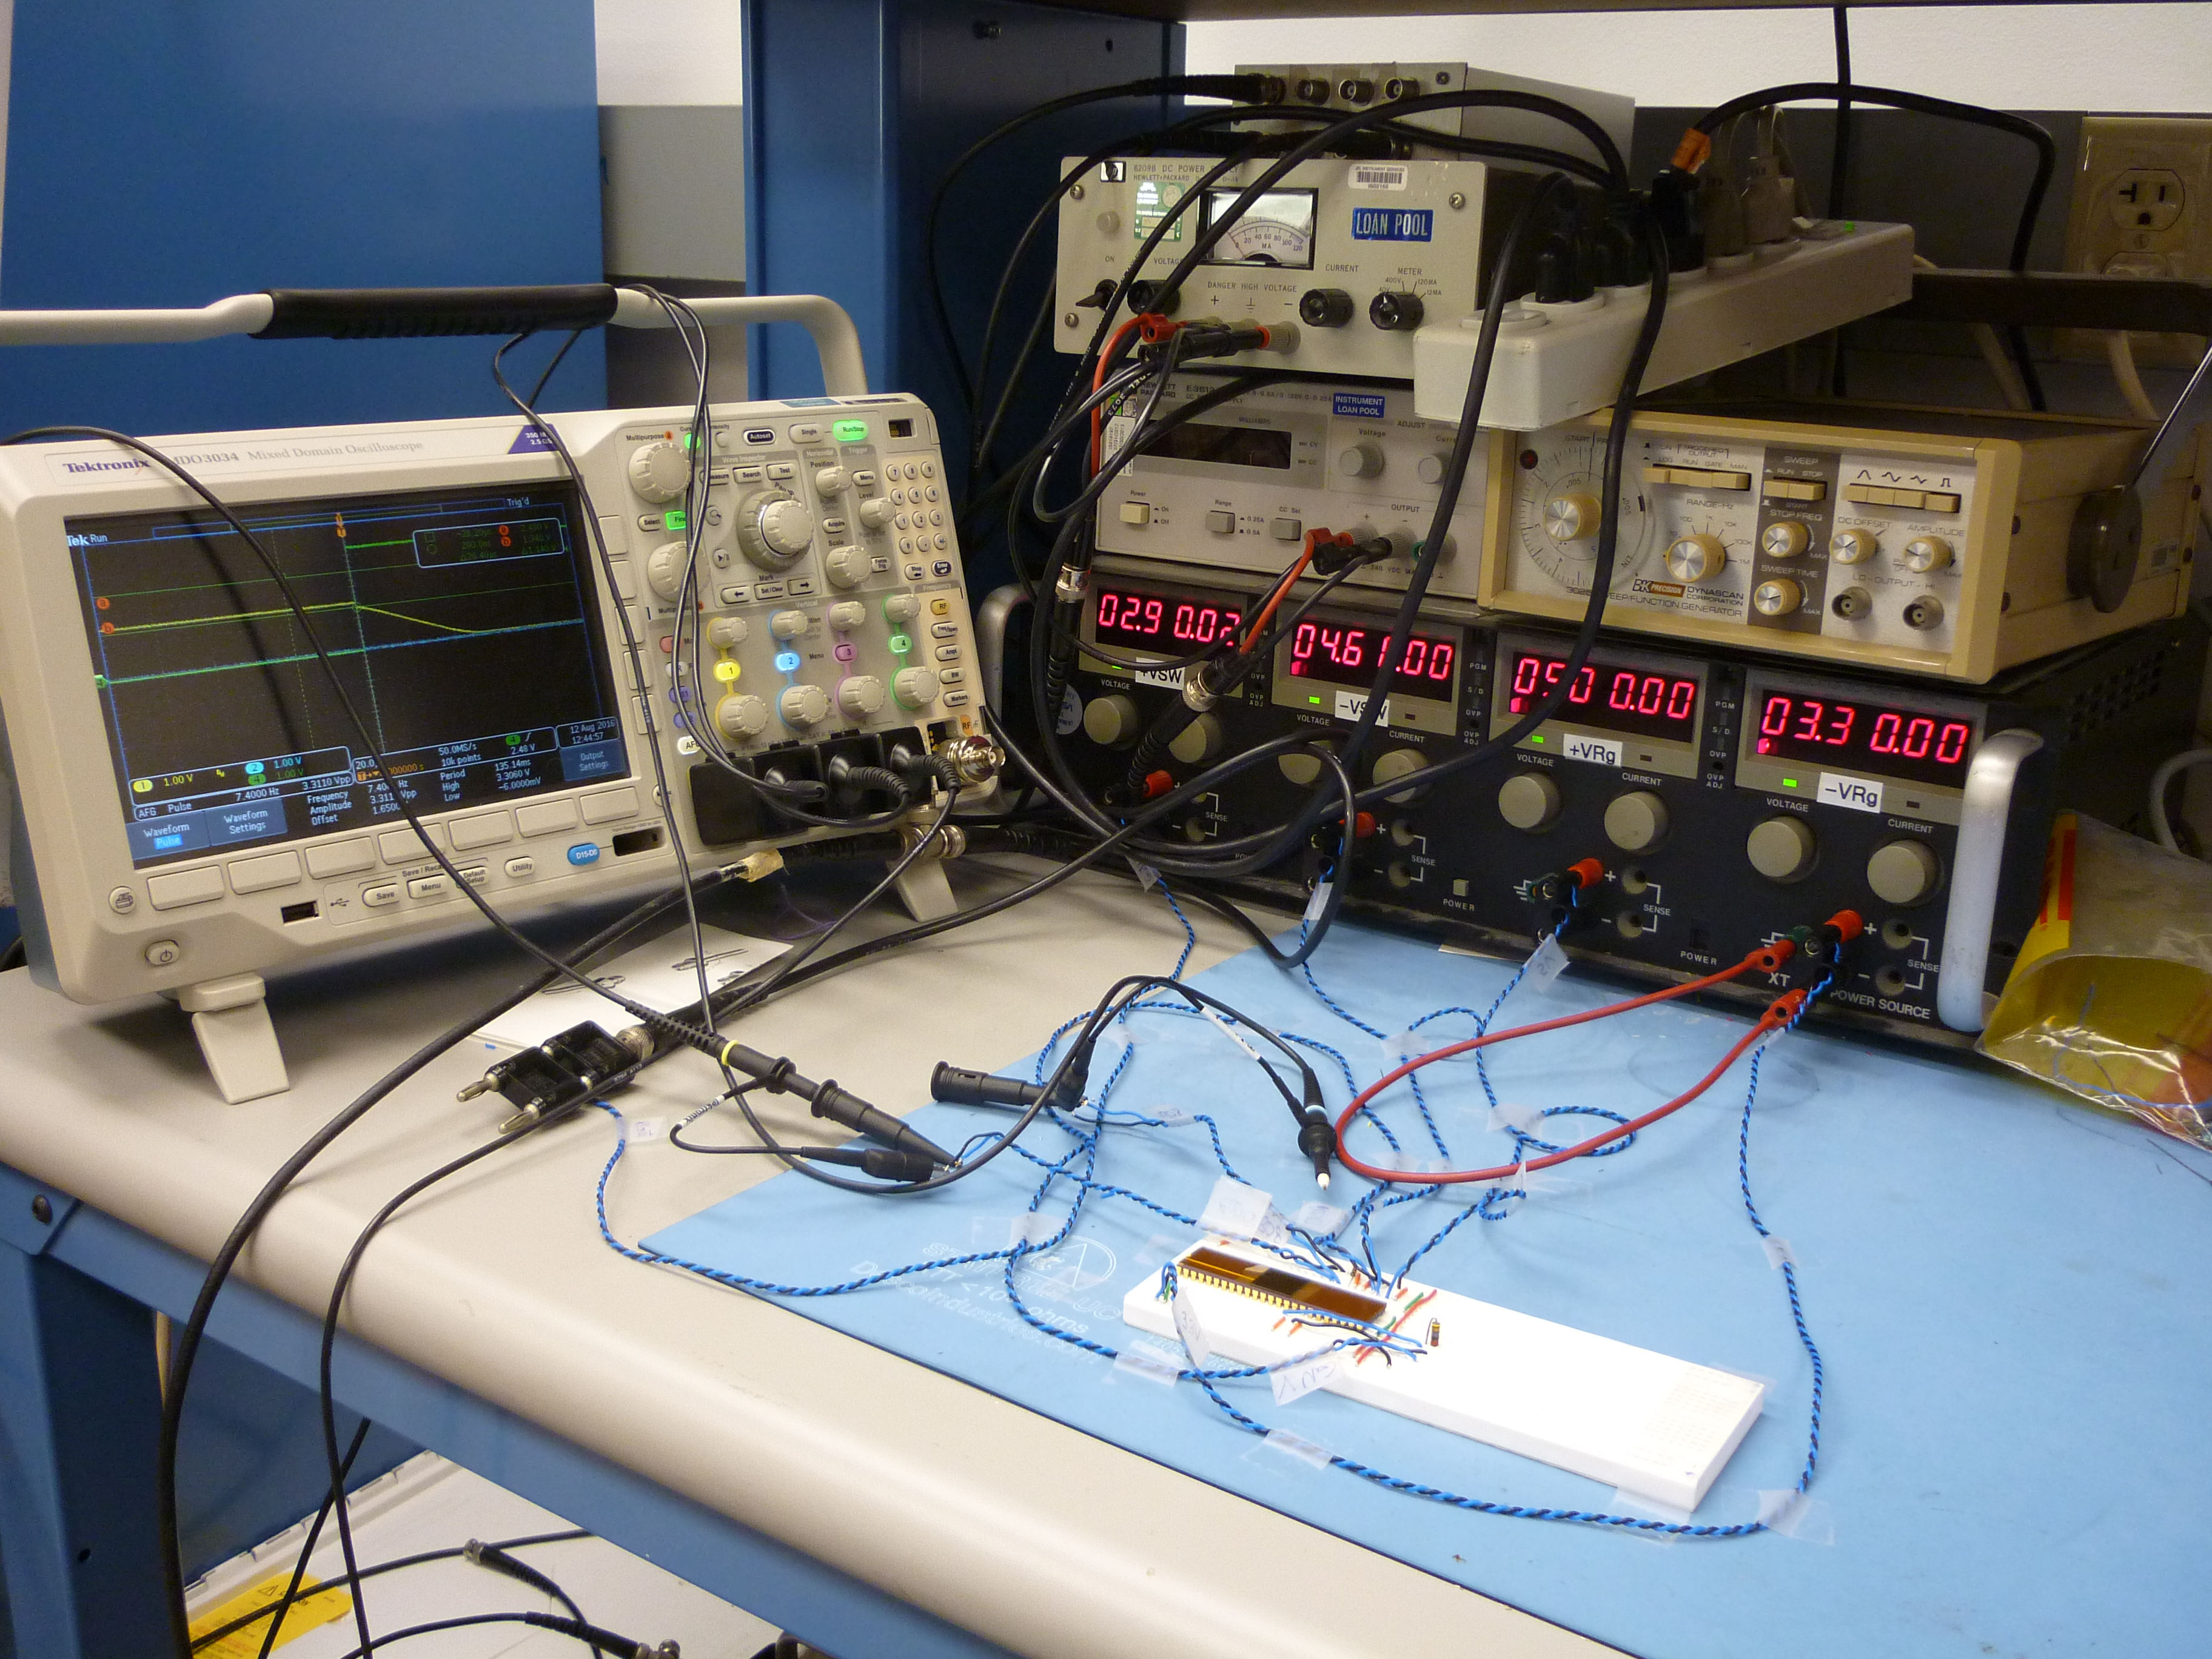
\includegraphics[width=0.6\linewidth]{fig/P1010158.JPG}
	\caption{setup overview}
	\label{fig:setup_overview}
\end{figure}

\begin{figure}[h]
	\centering
	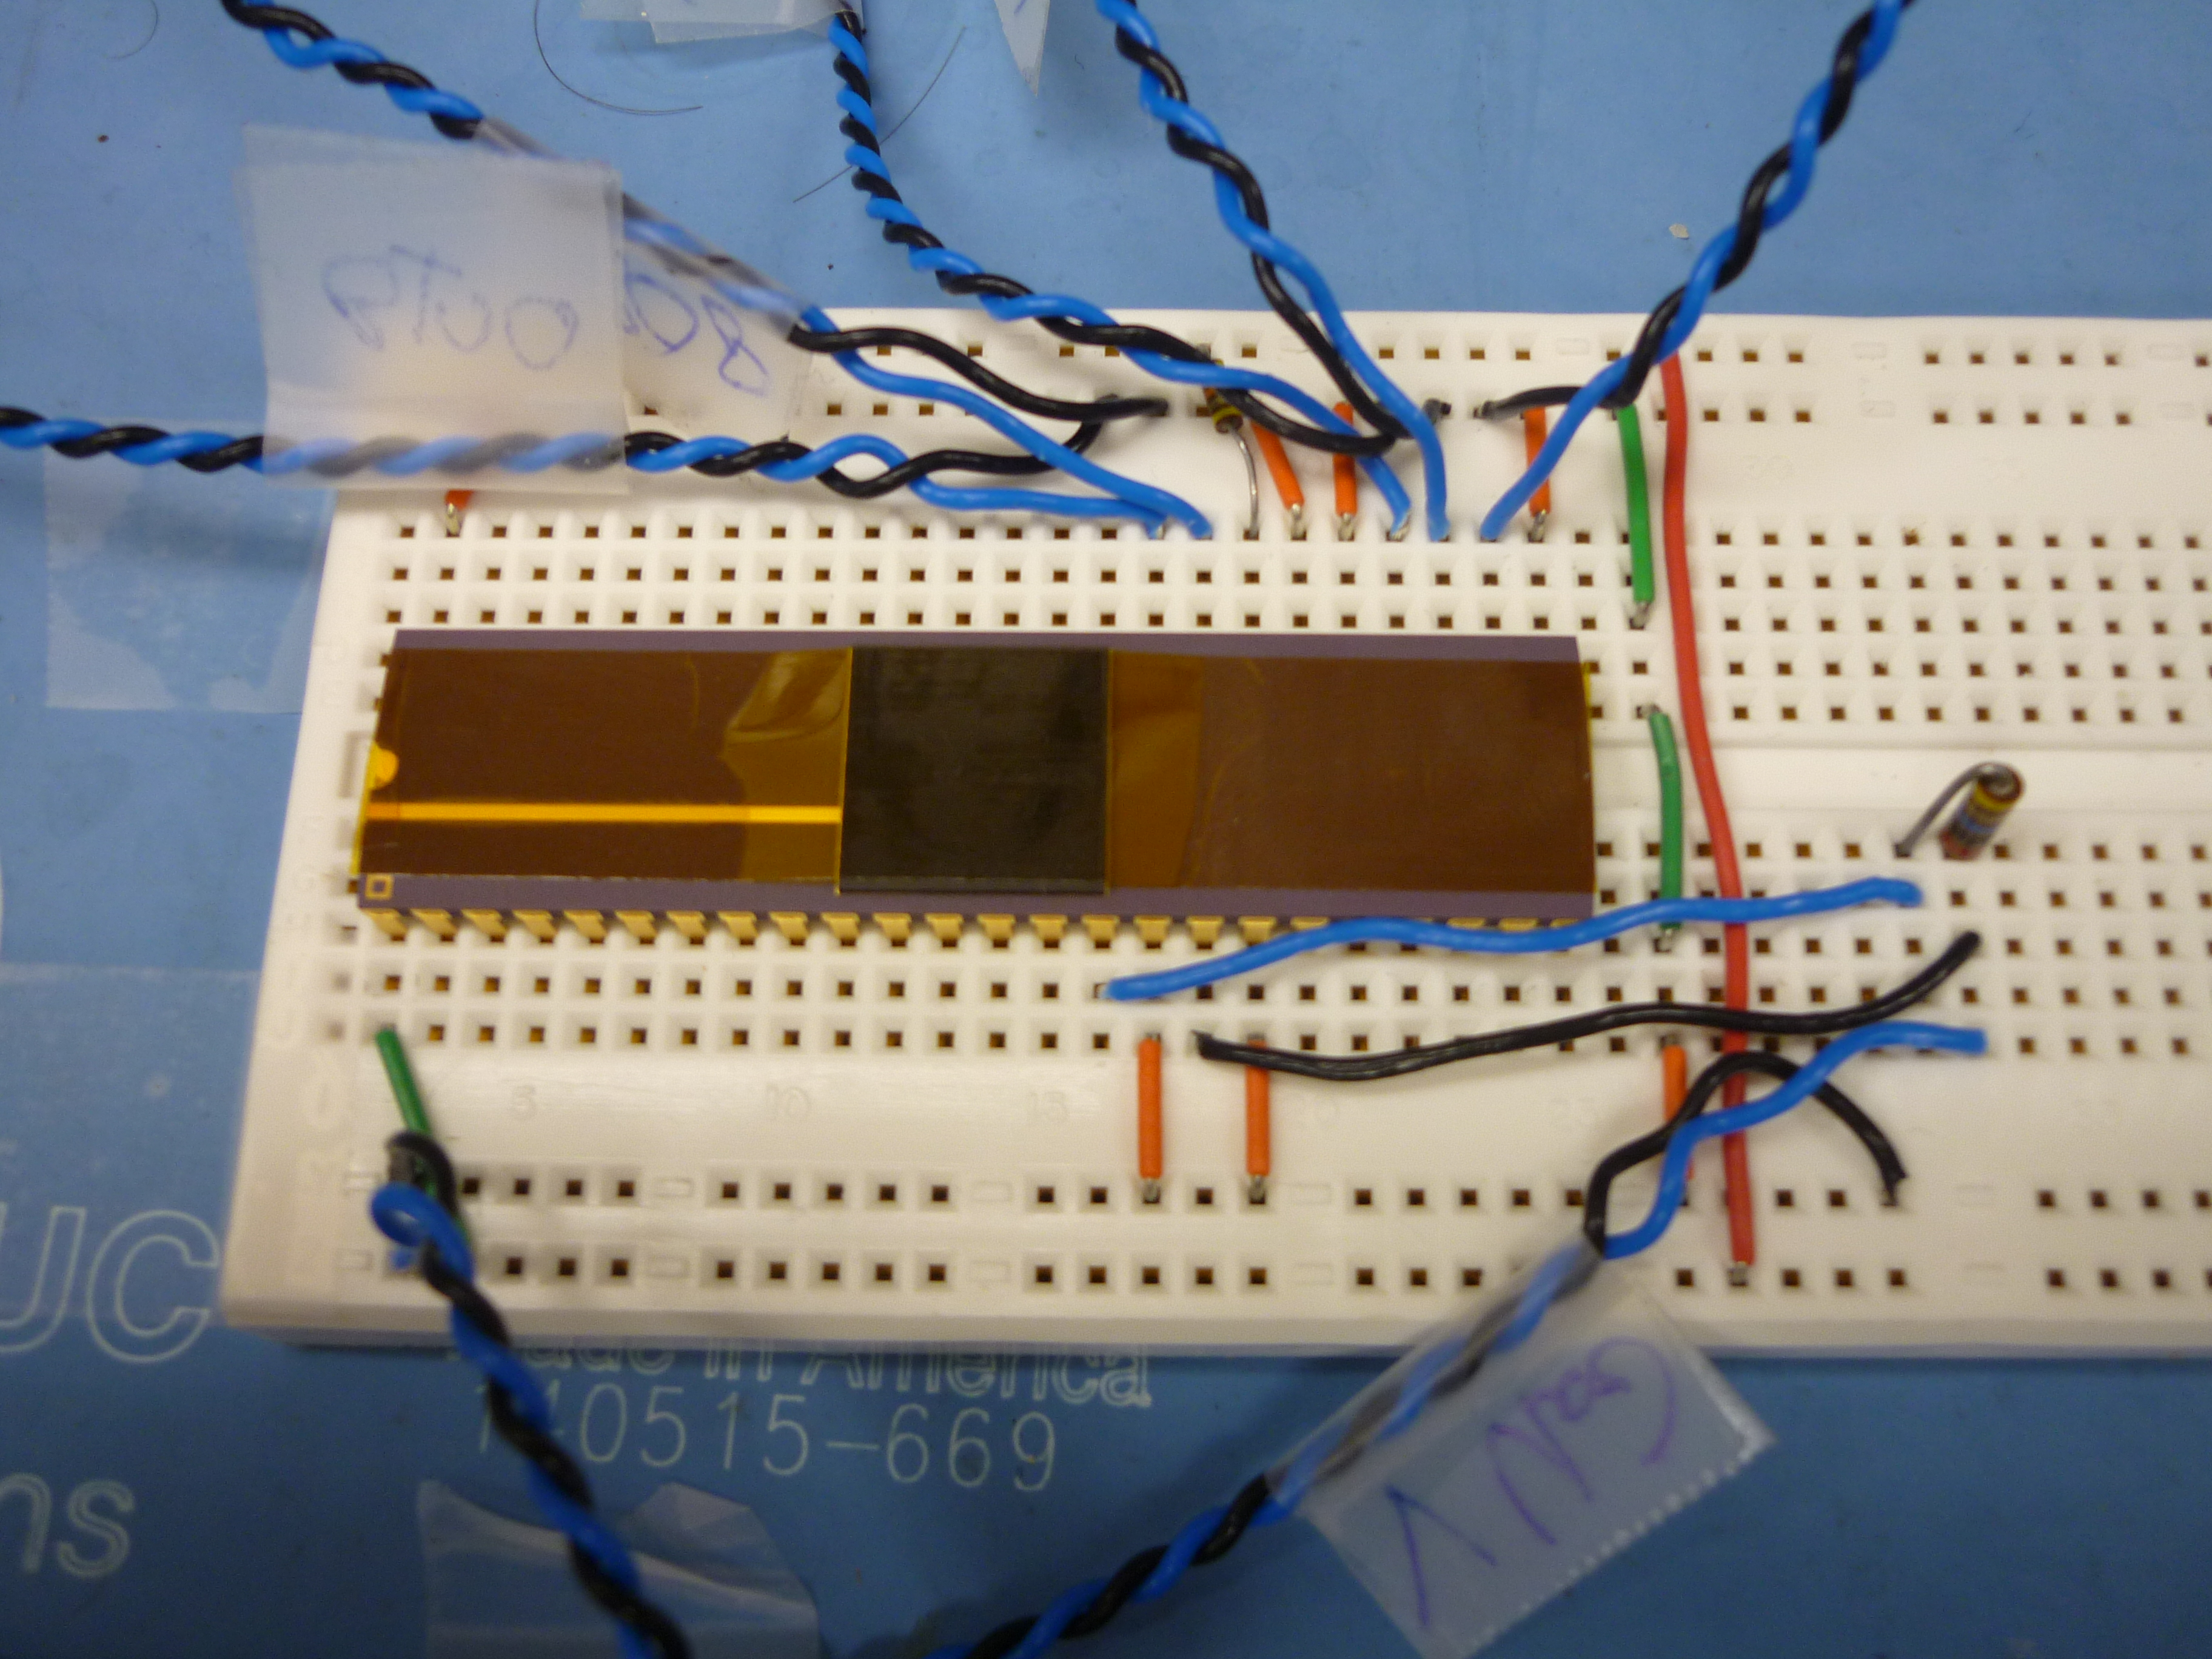
\includegraphics[width=0.6\linewidth]{fig/P1010159.JPG}
	\caption{close-up}
	\label{fig:close-up}
\end{figure}



% \section{setup}\label{sec:setup}
% \begin{figure}[H]
\centering
\usetikzlibrary{shapes,snakes}
\tikzstyle{dot} = [draw,shape=circle,fill=black, scale =.2]
\tikzstyle{l_arrow} = [draw,fill = black, regular polygon,regular polygon sides=3, rotate=-90, anchor=south, scale=.5] 
\tikzstyle{l_text} = [anchor=south west]
\tikzstyle{r_arrow} = [draw,fill = black, regular polygon,regular polygon sides=3, rotate=90, anchor=south, scale=.5] 
\tikzstyle{r_text} = [anchor=south east]
\begin{tikzpicture}[scale=1.5, every node/.style={scale=1}]


\node[l_text] at (-3,1) {VDD 3.3 (1)};
\node[l_text] at (-3,0) {IN[8] (15)};
\node[l_text] at (-3,-1) {VSUB (16)};
\node[l_text] at (-3,-2) {VDD\_HV (17)};
\node[l_text] at (-3,-3) {GND\_HV (18)};

\node[l_arrow] at (-3,1) {};
\node[l_arrow] at (-3,0) {};
\node[l_arrow] at (-3,-1) {};
\node[l_arrow] at (-3,-2) {};
\node[l_arrow] at (-3,-3) {};

\node[r_text] at (0,1) {(25) gnd};
\node[r_text] at (0,0) {(26) VDD5};
\node[r_text] at (0,-1) {(27) Vg};
\node[r_text] at (0,-2) {(28) Rst[3]};
\node[r_text] at (0,-3) {(29) Rst[1]};
\node[r_text] at (0,-4) {(30) Rst[2]};
\node[r_text] at (0,-5) {(31) Res};
\node[r_text] at (0,-6) {(32) VB0[8]};
\node[r_text] at (0,-7) {(33) out[8]};
\node[r_text] at (0,-8) {(48) gnd};


\node[r_arrow] at (0,1) {};
\node[r_arrow] at (0,0) {};
\node[r_arrow] at (0,-1) {};
\node[r_arrow] at (0,-2) {};
\node[r_arrow] at (0,-3) {};
\node[r_arrow] at (0,-4) {};
\node[r_arrow] at (0,-5) {};
\node[r_arrow] at (0,-6) {};
\node[r_arrow] at (0,-7) {};
\node[r_arrow] at (0,-8) {};
\draw  (-3,2) rectangle (0,-8);




\draw (-3.5,-1) node[ground]{} to (-3,-1);
\draw (-3.5,-3) node[ground]{} to (-3,-3);
\draw (0.5,1) node[ground]{} to (0,1);
\draw (0.5,-8) node[ground]{} to (0,-8);
\draw (0.5,-3) node[ground]{} to (0,-3);
\draw (0.5,-4) node[ground]{} to (0,-4);

\draw (0.5,0.25) node[anchor=south]{$5\,V$} (0.5,0.25) node[tground]{} to (0.5,0)to (0,0); % VDD5
\draw (0.5,-0.75) node[anchor=south]{$4.5\,V$} (0.5,-0.75) node[tground]{} to (0.5,-1)to (0,-1); % Vg
\draw (-3.5,1.25) node[anchor=south]{$3.3\,V$} (-3.5,1.25) node[tground]{} to (-3.5,1)to (-3,1); % VDD3.3
\draw (-3.5,-1.75) node[anchor=south]{$5\,V$} (-3.5,-1.75) node[tground]{} to (-3.5,-2)to (-3,-2); %VDD_HV
\draw (-4.5,0.25) node[anchor=south]{$set$} (-4.5,0.25) node[tground]{} to (-4.5,0)to (-4.5,0); % IN[8]
\draw (0.5,-1.75) node[anchor=south]{$reset$} (0.5,-1.75) node[tground]{} to (0.5,-2)to (0,-2); % Rst[3]
\draw  (0,-5) to[R=$50\,k\Omega$](1.5,-5) to (1.5,-4.75) node[tground]{} (1.5,-4.75) node[anchor=south]{$5\,V$}; %res


\draw (-4.5,0) to [R=$20\,M\Omega$](-3,0);

\end{tikzpicture}
\caption{Schematic of breadbord}
\label{tkz:breadbord}
\end{figure}
% \begin{figure}[H]
\centering
\usetikzlibrary{shapes,snakes}
\tikzstyle{dot} = [draw,shape=circle,fill=black, scale =.3]
\tikzstyle{l_arrow} = [draw,fill = black, regular polygon,regular polygon sides=3, rotate=-90, anchor=south, scale=.5] 
\tikzstyle{l_text} = [anchor=south west]
\tikzstyle{r_arrow} = [draw,fill = black, regular polygon,regular polygon sides=3, rotate=90, anchor=south, scale=.5] 
\tikzstyle{r_text} = [anchor=south east]
\begin{tikzpicture}[scale=1, every node/.style={scale=1}]

\draw[dashed, color=blue]  (-0.5,5.5) rectangle (0.5,-2);
\fill[color=blue, opacity=.1]  (-0.5,5.5) rectangle (0.5,-2);
\node[align=center, anchor=south] at (0,5.5) {voltage\\limiter};

\draw[dashed, color=green]  (1.25,5.5) rectangle (5.25,-2);
\fill[opacity=.1, color=green]  (1.25,5.5) rectangle (5.25,-2);
\node[align=center, anchor=south] at (3.25,5.5) {integrator};



\draw[dashed, color=red]  (5.75,5.5) rectangle (9.25,-2);
\fill[opacity=.1, color=red] (5.75,5.5) rectangle (9.25,-2);
\node[align=center, anchor=south] at (7.5,5.5) {current mirrors};

%\draw (0,0) to node[nfet]{};

%\draw (0,0) to (mos1.s);
\node(Vg)[nfet, rotate=-90] at (0,2.5) {};
\node[nfet, rotate=-90] (Reset) at (2.5,2) {};
\node[pfet] (CM_H1) at (5,3) {};
\node[nfet] (CM_L1) at (5,-1) {};
\node[nfet] (CM_H2) at (7,3) {};
\node[nfet] (CM_L2) at (7,-1) {};
\node[nfet] (CM_H3) at (9,3) {};
\node[nfet] (CM_L3) at (9,-1) {};



\draw (-1,2.5) node[anchor=east]{IN[i]} to (Vg.S);
\draw (Vg.G) |- (0,4.5) node[anchor=south]{Vg};
\draw (Vg.B) |- (1,2.5) node[dot]{} |- (CM_H1.G); %top
\draw (1,2.5) |- (1,0.5)  to [C=$450\,fF$](4,0.5) -| (CM_H1.D);
\draw (1.5,0.5) node[dot]{} -| (1.5,2) |- (Reset.B);
\draw (Reset.G) to (2.5,4.5) node[anchor=south]{Rst[3]};
\draw (Reset.D) -| (3.5,0.5) node[dot]{};
\draw (5,0.5) node[dot]{} to (CM_L1.D);
\draw (CM_L1.G) to (4,4.5) node[anchor=south]{Res}; 
\draw (CM_L1.S) to (CM_L2.S) to (7,-2.5) node[anchor=north]{gnd};
\draw (CM_H1.B) |- (CM_H2.D) to (7,4.5) node[anchor=south]{VDD3.3};
\draw (CM_L2.G) |- (4,0) node[dot]{};
\draw (5,0.5) -| (CM_H2.G);
\draw (CM_L1.B) to (CM_L1.S);
\draw (CM_L2.B) to (CM_L2.S);
\draw (CM_H2.B) to (CM_L2.D);
\draw (CM_H3.B) to (CM_L3.D);
\draw (1,3)node[dot]{} |- (8,4) |- (CM_H3.G);
\draw (CM_H3.D) |- (CM_H2.D) node[dot]{};
\draw (CM_L3.S) |- (CM_L2.S) node[dot]{};
\draw (CM_L3.G) |- (6,0) node[dot]{};
\draw (7,1.5)node[dot]{} to (10,1.5) node[anchor=west]{OUT[i]};
\draw (9,1)node[dot]{} to (10,1) node[anchor=west]{VBO[i]};



\end{tikzpicture}\caption{Schematic of ROIC channel}
\label{tkz:schematic_ROIC}
\end{figure}

% 
% \begin{figure}[h]
	% \centering
	% 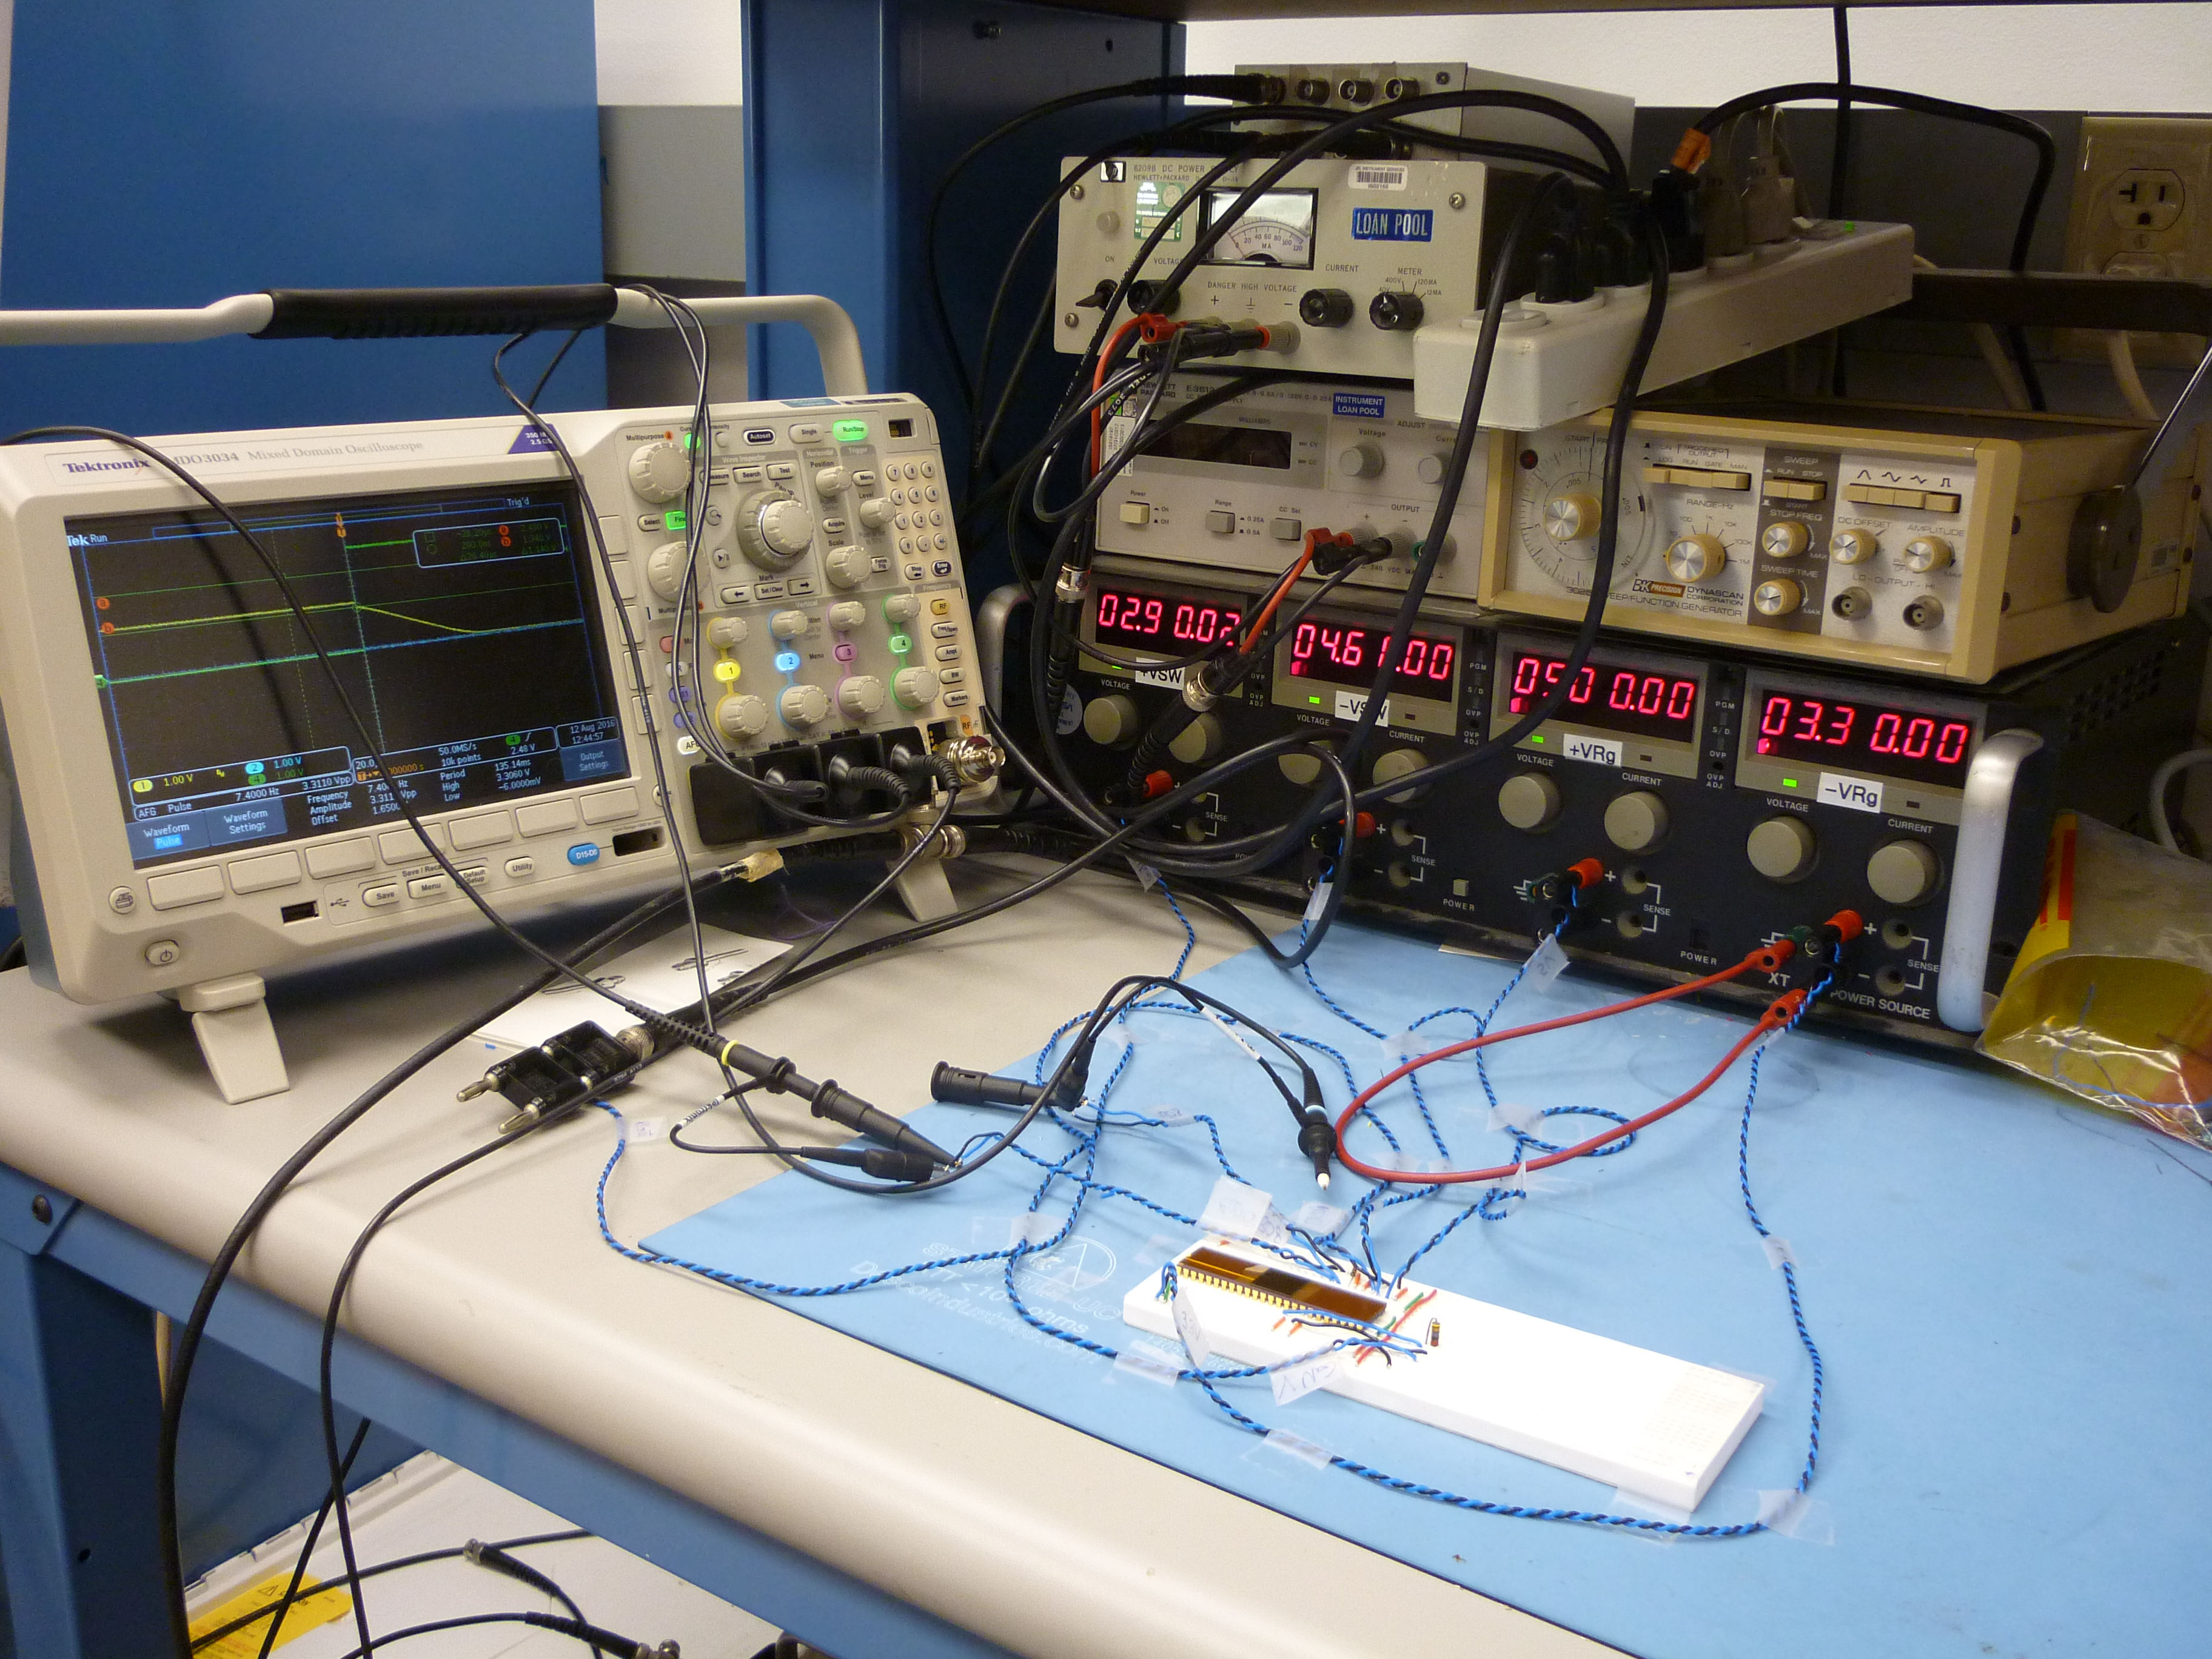
\includegraphics[width=0.6\linewidth]{fig/P1010158.JPG}
	% \caption{setup overview}
	% \label{fig:setup_overview}
% \end{figure}
% 
% \begin{figure}[h]
	% \centering
	% 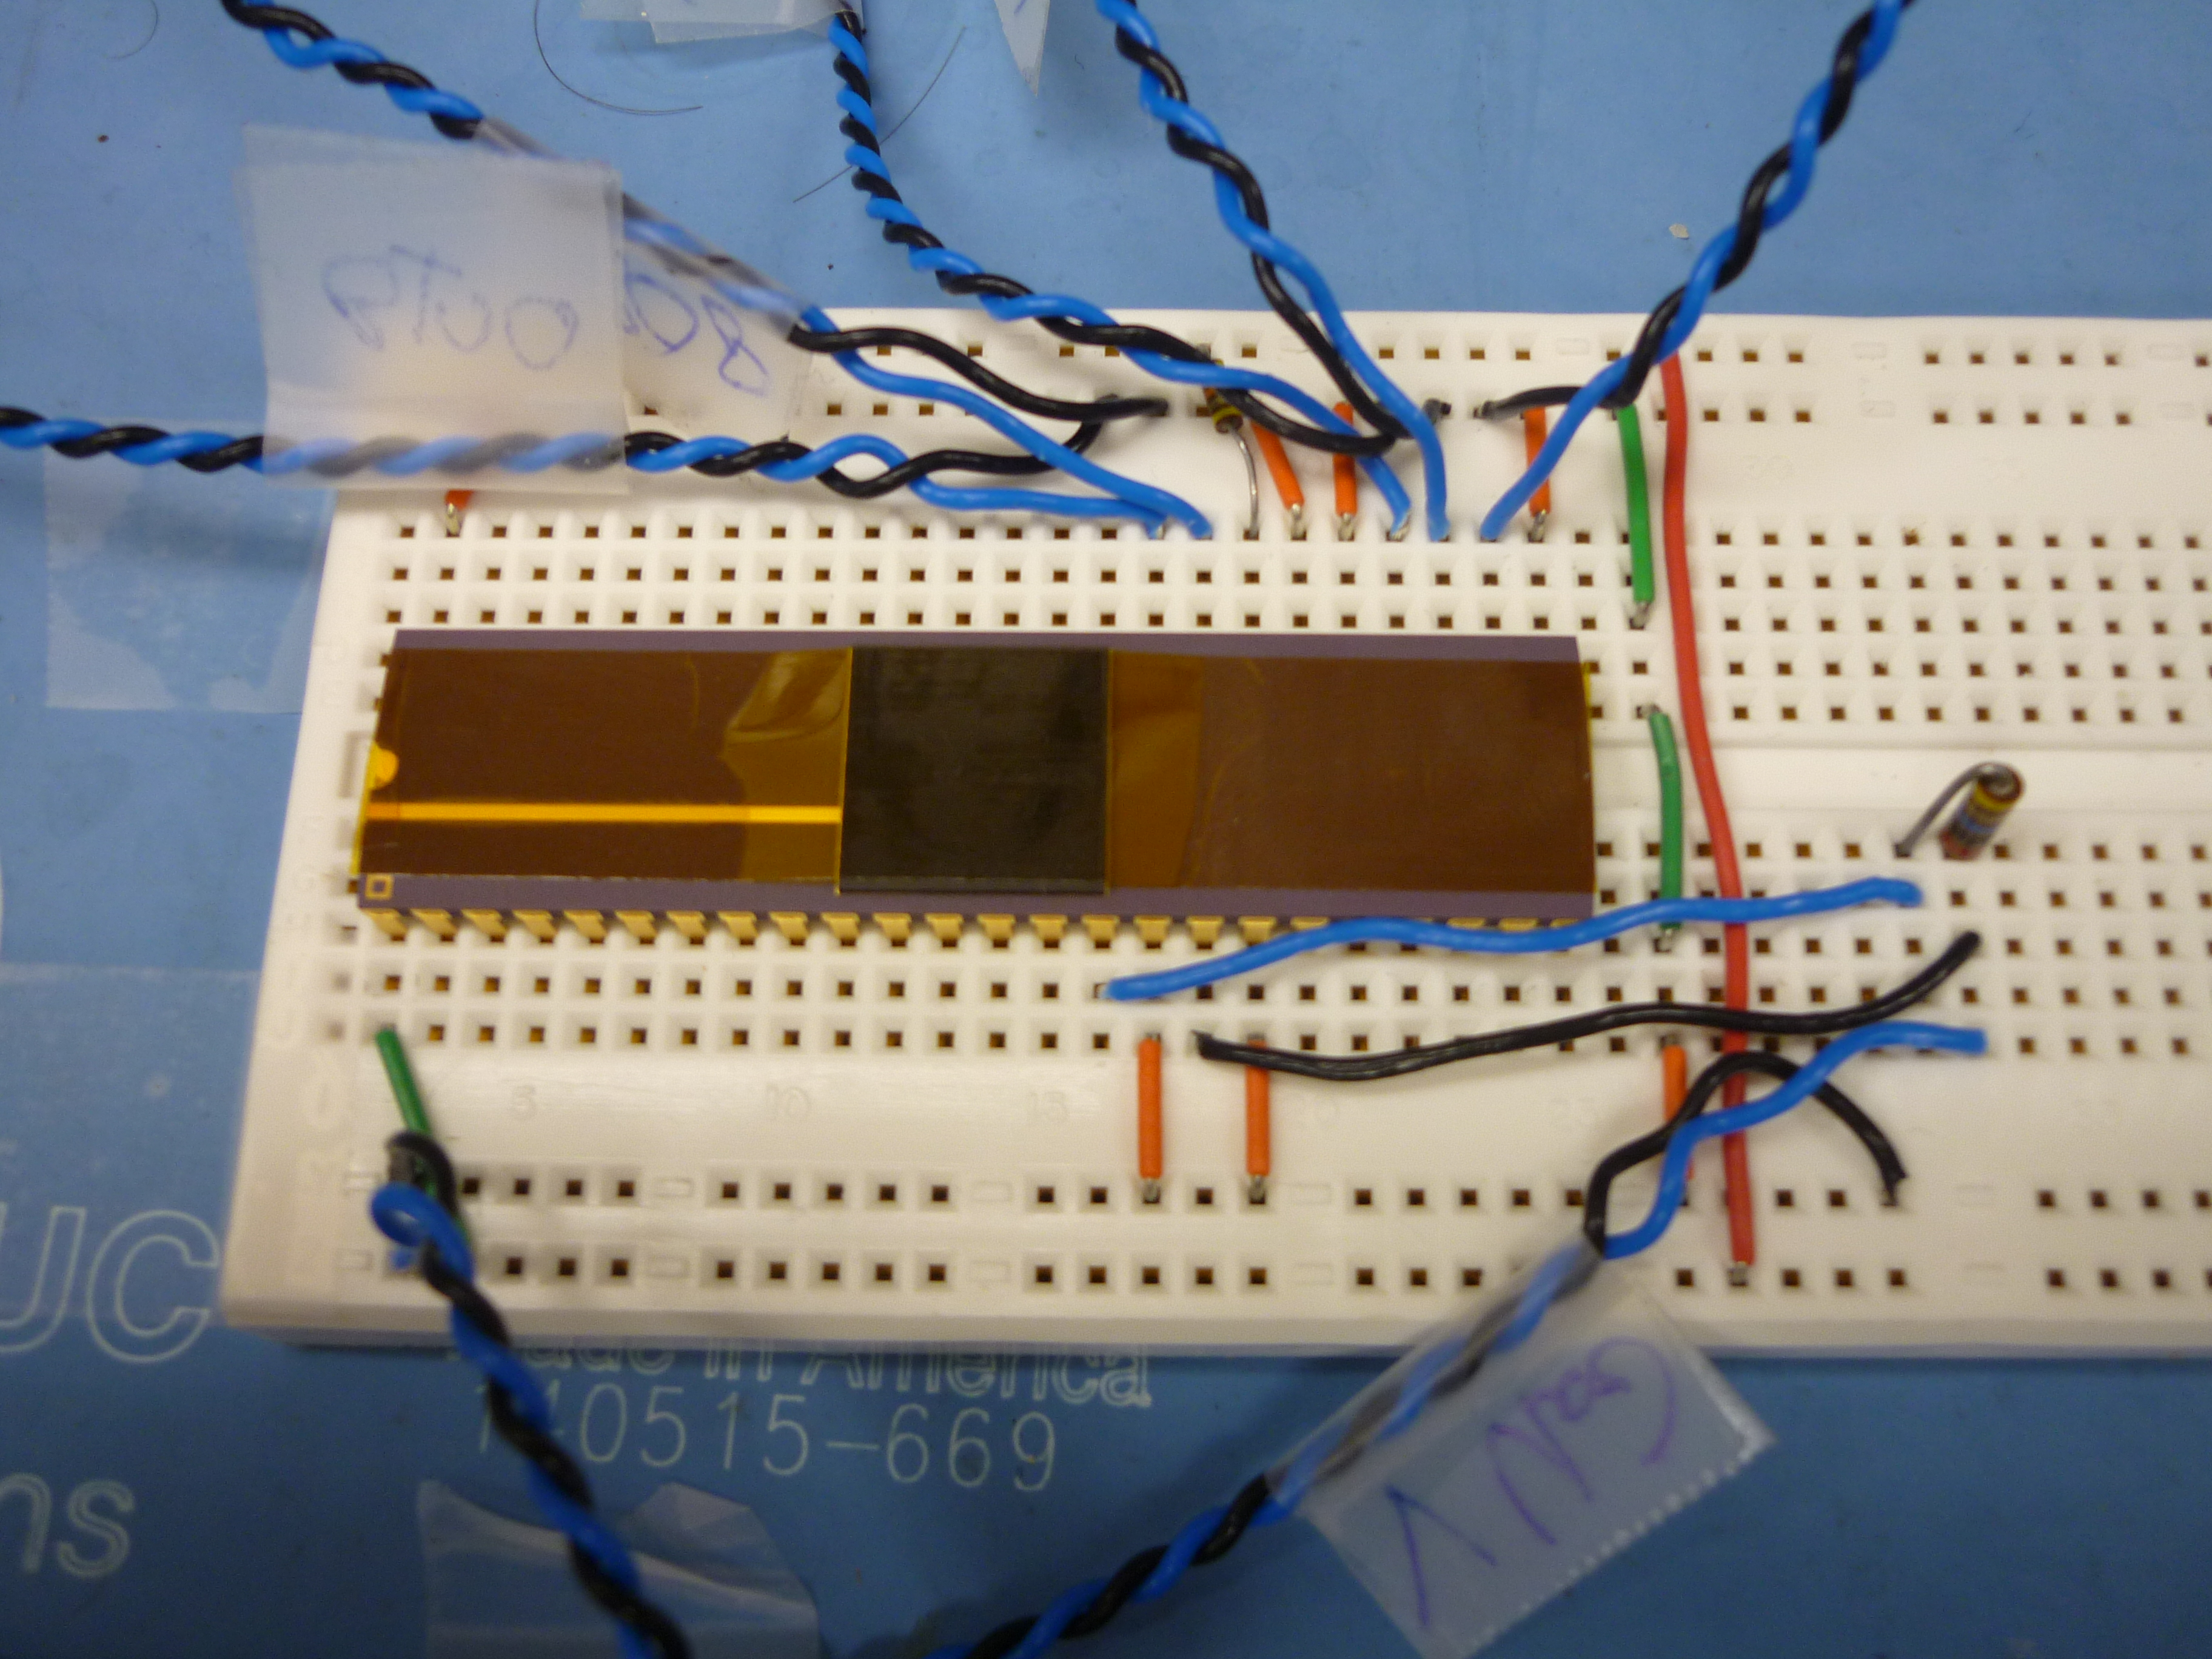
\includegraphics[width=0.6\linewidth]{fig/P1010159.JPG}
	% \caption{close-up}
	% \label{fig:close-up}
% \end{figure}

\clearpage

\section{Characterization for high impedance voltage source}
This section aims to characterize the behavior of the ROIC while exposed to a voltage source with a high resistance in the order of several $M\Omega$. A focus is put onto the performance in reset state, the relationshiop between input current and output voltage, and the current limiting properties of the input transistor.

\subsection{Reset}
This mesaurement addresses the behavior of the circuit in reset mode. \Cref{tkz:schematic_ROIC_reset} shows the measured values during reset mode. Note that the input voltage is $2.4\,V$, which is important when calculating the input current. 

\begin{figure}[H]
\centering

\usetikzlibrary{shapes,snakes}

\newcommand*{\Vg}{Vg\\ $\color{red}4.5\,V$}
\newcommand*{\Rst}{Rst[3]\\ $\color{red}0\,V$} 
\newcommand*{\Res}{Res\\ $\color{red}0.86\,V$}
\newcommand*{\VDD}{VDD3.3\\ $\color{red}3.3\,V$}
\newcommand*{\IN}{IN[i]\\ $\color{red}2.4\,V$}
\newcommand*{\OUT}{OUT[i] $\color{red}1.4\,V$}
\newcommand*{\VBO}{VBO[i] $\color{red}1.4\,V$}
\newcommand*{\gnd}{gnd\\ $\color{red}0\,V$}
\newcommand*{\C}{$\color{red}450\,fF$}




\tikzstyle{dot} = [draw,shape=circle,fill=black, scale =.3]
\tikzstyle{l_arrow} = [draw,fill = black, regular polygon,regular polygon sides=3, rotate=-90, anchor=south, scale=.5] 
\tikzstyle{l_text} = [anchor=south west]
\tikzstyle{r_arrow} = [draw,fill = black, regular polygon,regular polygon sides=3, rotate=90, anchor=south, scale=.5] 
\tikzstyle{r_text} = [anchor=south east]
\begin{tikzpicture}[scale=1, every node/.style={scale=1}]




\draw[dashed]  (-0.5,5.5) rectangle (0.5,-2);
\node[align=center, anchor=south] at (0,5.5) {voltage\\limiter};

\draw[dashed]  (1.25,5.5) rectangle (5.25,-2);
\node[align=center, anchor=south] at (3.25,5.5) {integrator};

\draw[dashed]  (5.75,5.5) rectangle (9.25,-2);
\node[align=center, anchor=south] at (7.5,5.5) {current mirrors};

%\draw (0,0) to node[nfet]{};

%\draw (0,0) to (mos1.s);
\node(Vg)[nfet, rotate=-90] at (0,2.5) {};
\node[nfet, rotate=-90] (Reset) at (2.5,2) {};
\node[pfet] (CM_H1) at (5,3) {};
\node[nfet] (CM_L1) at (5,-1) {};
\node[nfet] (CM_H2) at (7,3) {};
\node[nfet] (CM_L2) at (7,-1) {};
\node[nfet] (CM_H3) at (9,3) {};
\node[nfet] (CM_L3) at (9,-1) {};



\draw (-1,2.5) node[anchor=east, align=center]{\IN} to (Vg.S);
\draw (Vg.G) |- (0,4.5) node[anchor=south, align=center]{\Vg};
\draw (Vg.B) |- (1,2.5) node[dot]{} |- (CM_H1.G); %top
\draw (1,2.5) |- (1,0.5)  to [C=\C](4,0.5) -| (CM_H1.D);
\draw (1.5,0.5) node[dot]{} -| (1.5,2) |- (Reset.B);
\draw (Reset.G) to (2.5,4.5) node[anchor=south, align=center]{\Rst};
\draw (Reset.D) -| (3.5,0.5) node[dot]{};
\draw (5,0.5) node[dot]{} to (CM_L1.D);
\draw (CM_L1.G) to (4,4.5) node[anchor=south, align=center]{\Res}; 
\draw (CM_L1.S) to (CM_L2.S) to (7,-2.5) node[anchor=north, align=center]{\gnd};
\draw (CM_H1.B) |- (CM_H2.D) to (7,4.5) node[anchor=south, align=center]{\VDD};
\draw (CM_L2.G) |- (4,0) node[dot]{};
\draw (5,0.5) -| (CM_H2.G);
\draw (CM_L1.B) to (CM_L1.S);
\draw (CM_L2.B) to (CM_L2.S);
\draw (CM_H2.B) to (CM_L2.D);
\draw (CM_H3.B) to (CM_L3.D);
\draw (1,3)node[dot]{} |- (8,4) |- (CM_H3.G);
\draw (CM_H3.D) |- (CM_H2.D) node[dot]{};
\draw (CM_L3.S) |- (CM_L2.S) node[dot]{};
\draw (CM_L3.G) |- (6,0) node[dot]{};
\draw (7,1.5)node[dot]{} to (10,1.5) node[anchor=west, align=center]{\OUT};
\draw (9,1)node[dot]{} to (10,1) node[anchor=west, align=center]{\VBO};




\end{tikzpicture}

\caption{Schematic of ROIC channel template}
\label{tkz:schematic_ROIC_reset}
\end{figure}



\subsection{Source follower}
There are two identical source followers per lane. We can use the VBO source follower to characterise both. This because the input can be directly controlled, and the output directly read. \Cref{fig:source_follower} shows both the measured data and a fitted line with the formula $vbo=0.827v_{in}-0.624$. It will be assumed that this line characterises the performance of both source followers for $1<v_{in}<4$.

\begin{figure}[h]
	    \centering
	    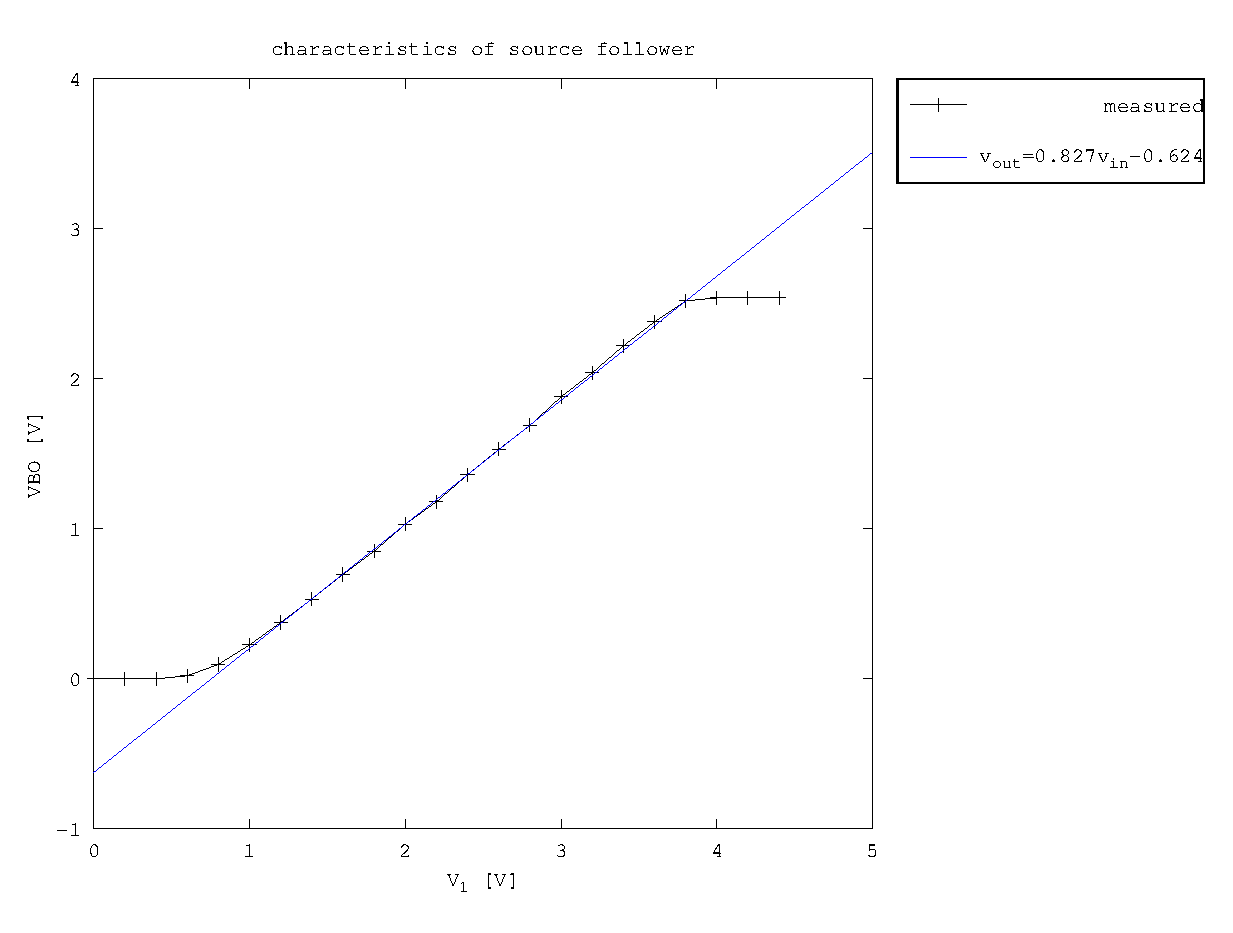
\includegraphics[width=\textwidth]{fig/source_follower.eps}
	    \caption[]%
	    {plot of the input voltage against VBO. This plot shows the characteristics of the voltage follower}    
	    \label{fig:source_follower}	
\end{figure}






\clearpage
\subsection{Standard performance}\label{ssec:standard}
This test aims to address the basic relationship between input current and output voltage. \Cref{tkz:integrator_test} shows the setup used for this test. Channel 8 was used, so the end of the $20\,M\Omega$ resistor is connected to IN[8], and probes are connected to OUT[8] and VBO[8]. 

\begin{figure}[H]
\centering

\usetikzlibrary{shapes,snakes}

\newcommand*{\Vg}{Vg\\ $\color{red}4.5\,V$}
\newcommand*{\Rst}{\textbf{Rst[3]}\\ $\color{blue}reset$} 
\newcommand*{\Res}{Res\\ $\color{red}0.86\,V$}
\newcommand*{\VDD}{VDD3.3\\ $\color{red}3.3\,V$}
\newcommand*{\IN}{$\color{blue}V_{in}$}
\newcommand*{\OUT}{$\color{blue}V_{out}$}
\newcommand*{\VBO}{\color{blue}\textbf{VBO[8]} $\color{red}1.4\,V$}
\newcommand*{\gnd}{gnd\\ $\color{red}0\,V$}
\newcommand*{\C}{$\color{blue}C$}




\tikzstyle{dot} = [draw,shape=circle,fill=black, scale =.3]
\tikzstyle{l_arrow} = [draw,fill = black, regular polygon,regular polygon sides=3, rotate=-90, anchor=south, scale=.5] 
\tikzstyle{l_text} = [anchor=south west]
\tikzstyle{r_arrow} = [draw,fill = black, regular polygon,regular polygon sides=3, rotate=90, anchor=south, scale=.5] 
\tikzstyle{r_text} = [anchor=south east]
\begin{tikzpicture}[scale=1, every node/.style={scale=1}]




\draw[dashed]  (-0.5,5.5) rectangle (0.5,-2);
\node[align=center, anchor=south] at (0,5.5) {voltage\\limiter};

\draw[dashed]  (1.25,5.5) rectangle (5.25,-2);
\node[align=center, anchor=south] at (3.25,5.5) {integrator};

\draw[dashed]  (5.75,5.5) rectangle (9.25,-2);
\node[align=center, anchor=south] at (7.5,5.5) {current mirrors};

%\draw (0,0) to node[nfet]{};

%\draw (0,0) to (mos1.s);
\node(Vg)[nfet, rotate=-90] at (0,2.5) {};
\node[nfet, rotate=-90] (Reset) at (2.5,2) {};
\node[pfet] (CM_H1) at (5,3) {};
\node[nfet] (CM_L1) at (5,-1) {};
\node[nfet] (CM_H2) at (7,3) {};
\node[nfet] (CM_L2) at (7,-1) {};
\node[nfet] (CM_H3) at (9,3) {};
\node[nfet] (CM_L3) at (9,-1) {};



\draw (-1,2.5) node[anchor=east, align=center]{} to (Vg.S);
\draw (Vg.G) |- (0,4.5) node[anchor=south, align=center]{\Vg};
\draw (Vg.B) |- (1,2.5) node[dot]{} |- (CM_H1.G); %top
\draw (1,2.5) |- (1,0.5)  to [C=\C](4,0.5) -| (CM_H1.D);
\draw (1.5,0.5) node[dot]{} -| (1.5,2) |- (Reset.B);
\draw (Reset.G) to (2.5,4.5) node[anchor=south, align=center]{\Rst};
\draw (Reset.D) -| (3.5,0.5) node[dot]{};
\draw (5,0.5) node[dot]{} to (CM_L1.D);
\draw (CM_L1.G) to (4,4.5) node[anchor=south, align=center]{\Res}; 
\draw (CM_L1.S) to (CM_L2.S) to (7,-2.5) node[anchor=north, align=center]{\gnd};
\draw (CM_H1.B) |- (CM_H2.D) to (7,4.5) node[anchor=south, align=center]{\VDD};
\draw (CM_L2.G) |- (4,0) node[dot]{};
\draw (5,0.5) -| (CM_H2.G);
\draw (CM_L1.B) to (CM_L1.S);
\draw (CM_L2.B) to (CM_L2.S);
\draw (CM_H2.B) to (CM_L2.D);
\draw (CM_H3.B) to (CM_L3.D);
\draw (1,3)node[dot]{} |- (8,4) |- (CM_H3.G);
\draw (CM_H3.D) |- (CM_H2.D) node[dot]{};
\draw (CM_L3.S) |- (CM_L2.S) node[dot]{};
\draw (CM_L3.G) |- (6,0) node[dot]{};
\draw (7,1.5)node[dot]{} to (10,1.5) node[anchor=west, align=center]{\OUT};
%\draw (9,1)node[dot]{} to (10,1) node[anchor=west, align=center]{\VBO};

\draw (-2.5,2.5)node[anchor=east, align=center]{\IN} to [R=$20\,M\Omega$](-1,2.5);


\end{tikzpicture}

\caption{Schematic of ROIC channel template}
\label{tkz:integrator_test}
\end{figure}


\Cref{fig:slopes} shows the time versus voltage plot of both the VBO and OUT for a constant input voltage. The rising and falling slopes are the VBO and OUt respecively. The timescale of this plot does not allow for much inside in VBO, but it does show some interesting results for the behavior of OUT. When the reset switches, the input node immediately loses some charge. Note that the osciloscope matches the rising edge of the rset signal to time is $0\,s$, so this drop is at $0\,s$. It is interesting to observe that the slope is constant for all input voltages. The slopes is much slower than the time necessary for the reset transistor to switch, so the observed slope is not limited by the reset transistor, but by the source follower that tries to keep up. This observed slope is therefore the maximum rate at which the output node can be pulled down in the current set-up.  lso note that the slope gets steeper when the integrator capacitance decreases. This is to be expected. However also note that the maximum slopes across the different capacitances are all identical.


\begin{figure}[h]
	\centering
	\begin{subfigure}[b]{0.475\textwidth}
	    \centering
	    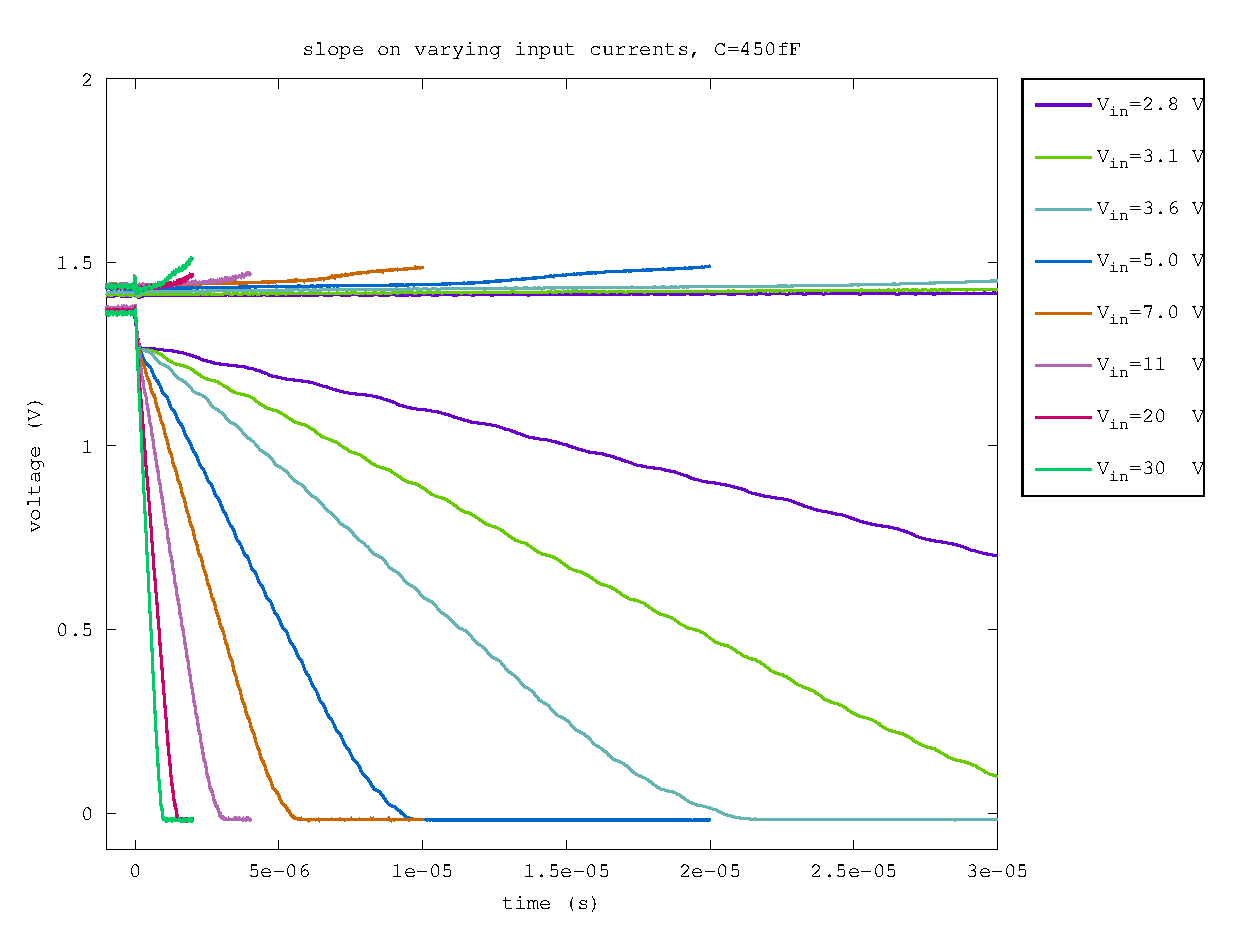
\includegraphics[width=\textwidth]{fig/slope_450fF.eps}
	    \caption[Network2]%
	    {$C=450\,fF$}    
	    \label{fig:slopes_450fF}
	\end{subfigure}
	\hfill
	\begin{subfigure}[b]{0.475\textwidth}  
	    \centering 
	    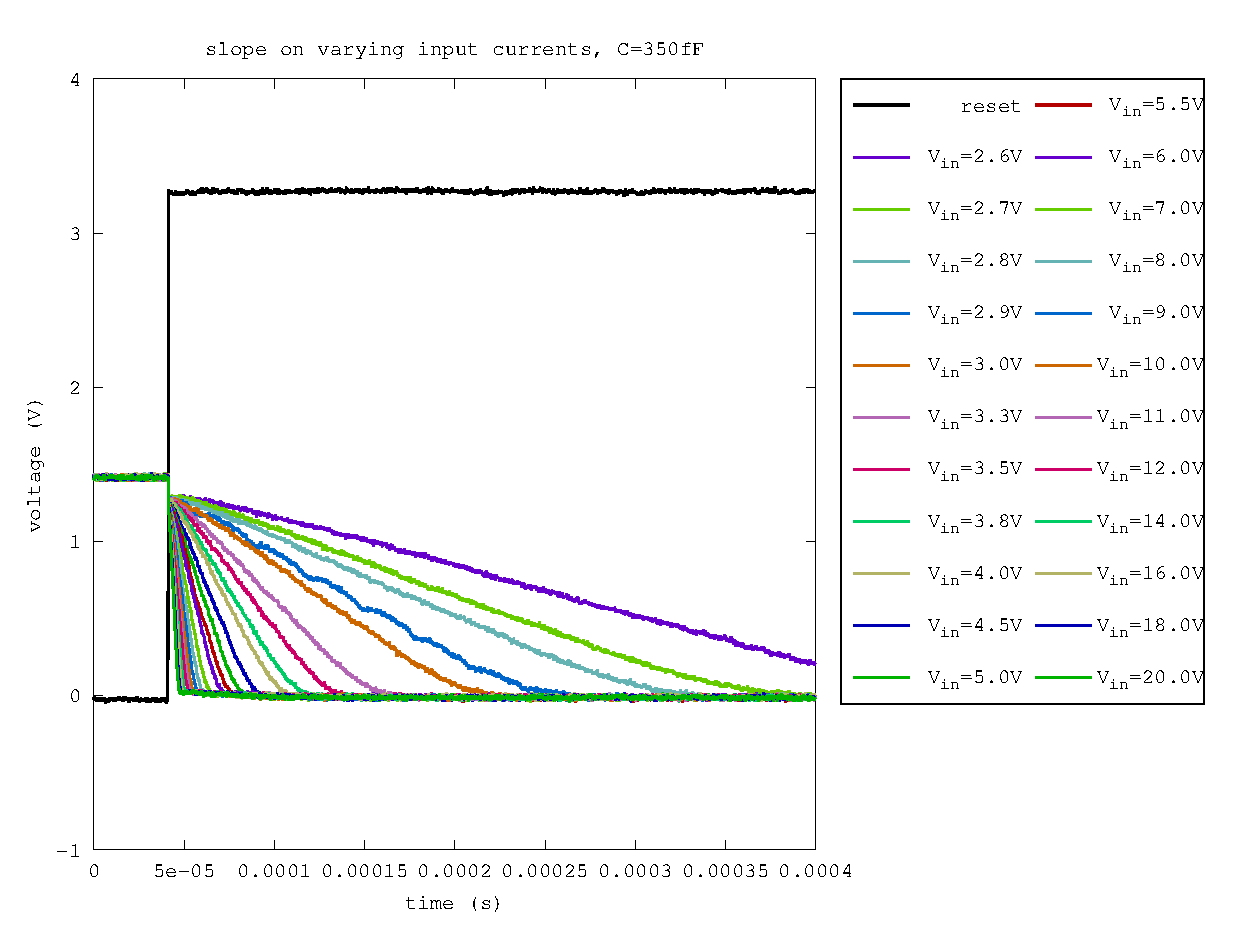
\includegraphics[width=\textwidth]{fig/slope_350fF.eps}
	    \caption[]%
	    {$C=350\,fF$}    
	    \label{fig:slopes_350fF}
	\end{subfigure}
	\vskip\baselineskip
	\begin{subfigure}[b]{0.475\textwidth}   
	    \centering 
	    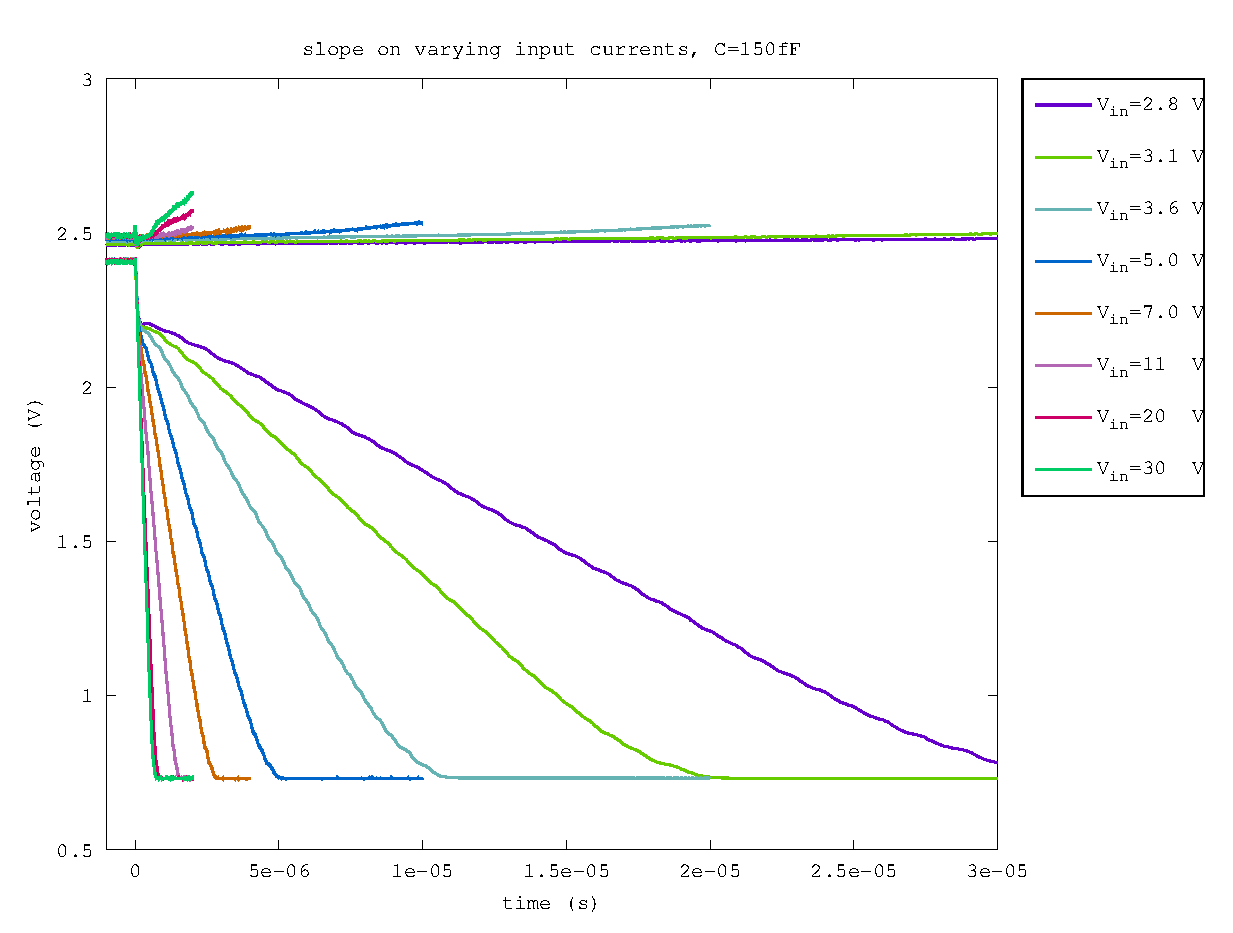
\includegraphics[width=\textwidth]{fig/slope_150fF.eps}
	    \caption[]%
	    {$C=150\,fF$}    
	    \label{fig:slopes_150fF}
	\end{subfigure}
	\quad
	\begin{subfigure}[b]{0.475\textwidth}   
	    \centering 
	    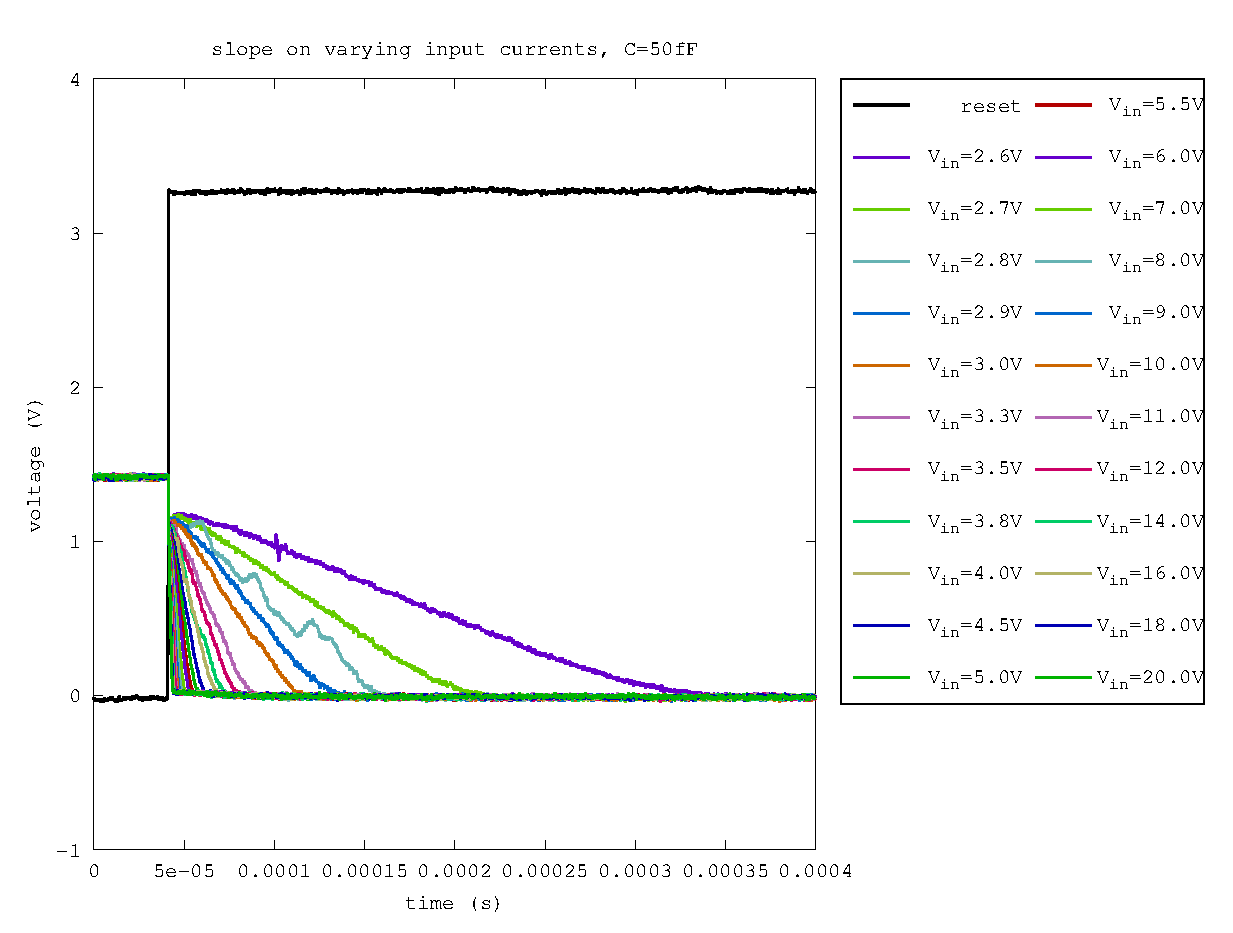
\includegraphics[width=\textwidth]{fig/slope_50fF.eps}
	    \caption[]%
	    {$C=50\,fF$}    
	    \label{fig:slopes_50fF}
	\end{subfigure}
	\caption{Expected versus measured charge up times for different input voltages. The input voltage is connected to the input through a resistor of $20\,M\Omega$}
	\label{fig:slopes}
\end{figure}

\Cref{fig:charges} shows the same plot as \cref{fig:slopes}, but now the x axis is scaled with input current. This shows for \cref{fig:slopes_450fF} and \ref{fig:slopes_350fF} that the relationship between output voltage and charge is equal across different input voltages. For \cref{fig:slopes_150fF} and \ref{fig:slopes_50fF} however, one can see that the higher voltages lose this property. Another intersting observation is that when one looks closely at the plot, one can observe a small oscillation with a period that is constant with charge. Also the period is constant across different voltages. A hypothesis explaining this behavior has yet to be found.


\begin{figure}[h]
	\centering
	\begin{subfigure}[b]{0.475\textwidth}
	    \centering
	    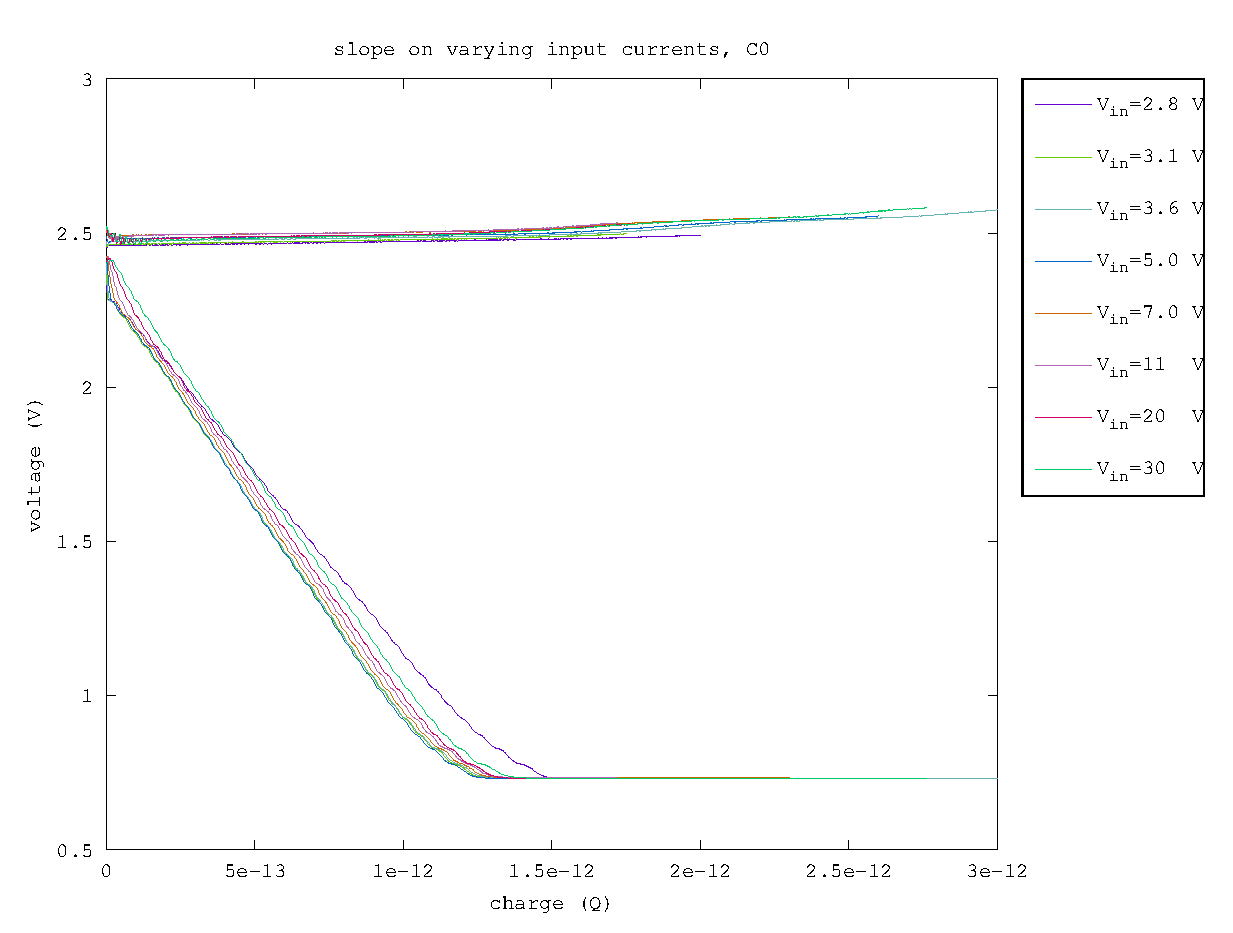
\includegraphics[width=\textwidth]{fig/charge_450fF.eps}
	    \caption[Network2]%
	    {$C=450\,fF$}    
	    \label{fig:charges_450fF}
	\end{subfigure}
	\hfill
	\begin{subfigure}[b]{0.475\textwidth}  
	    \centering 
	    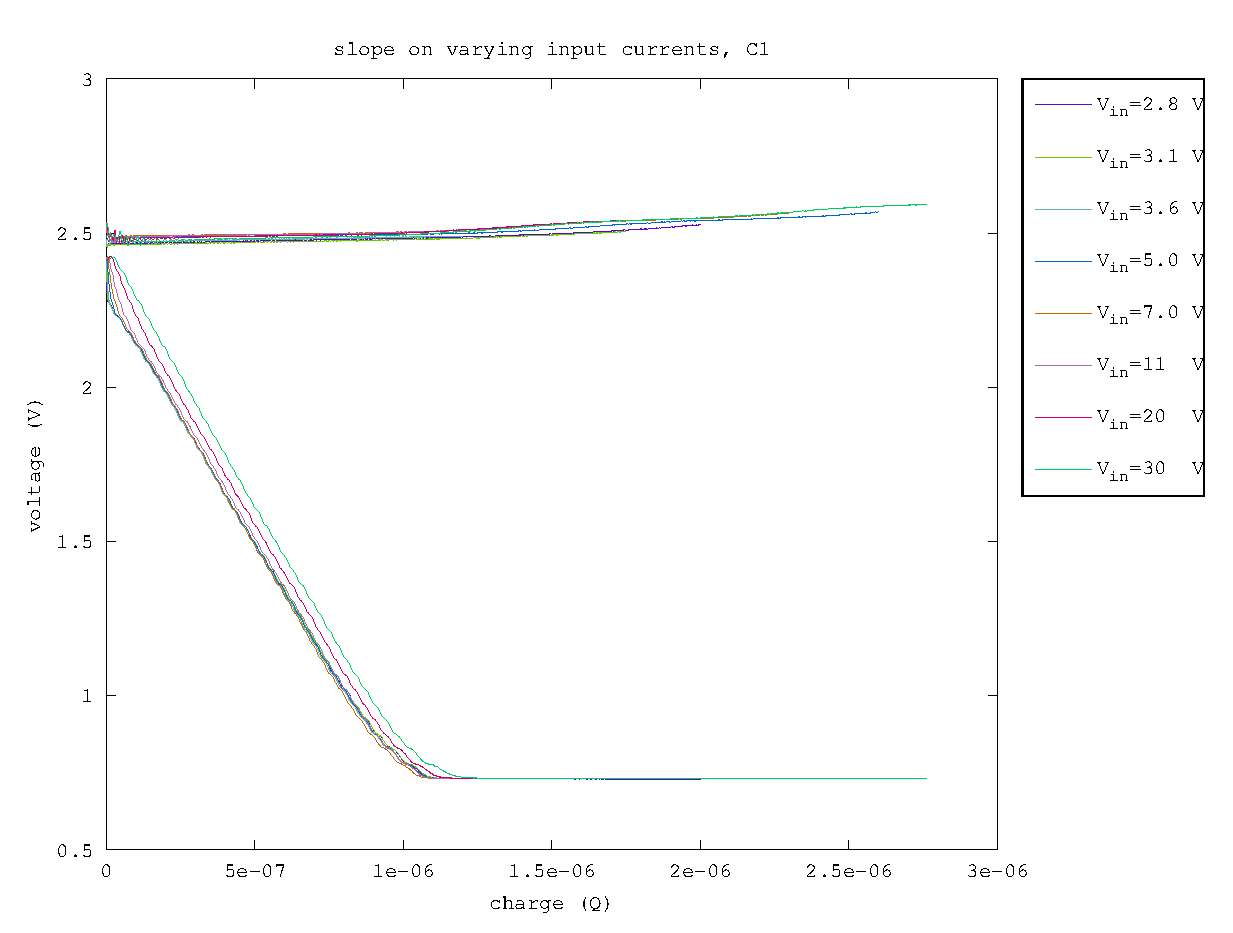
\includegraphics[width=\textwidth]{fig/charge_350fF.eps}
	    \caption[]%
	    {$C=350\,fF$}    
	    \label{fig:charges_350fF}
	\end{subfigure}
	\vskip\baselineskip
	\begin{subfigure}[b]{0.475\textwidth}   
	    \centering 
	    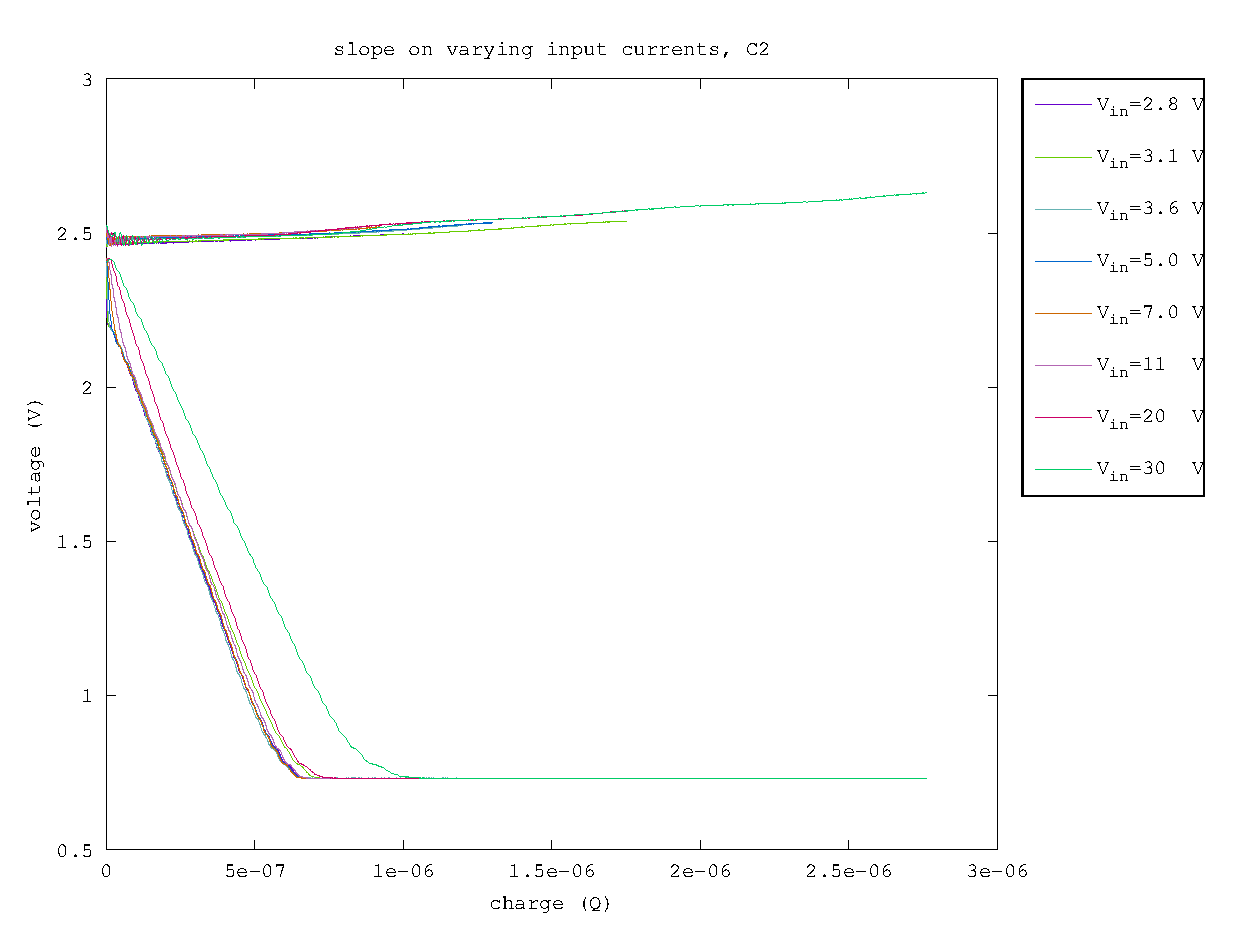
\includegraphics[width=\textwidth]{fig/charge_150fF.eps}
	    \caption[]%
	    {$C=150\,fF$}    
	    \label{fig:charges_150fF}
	\end{subfigure}
	\quad
	\begin{subfigure}[b]{0.475\textwidth}   
	    \centering 
	    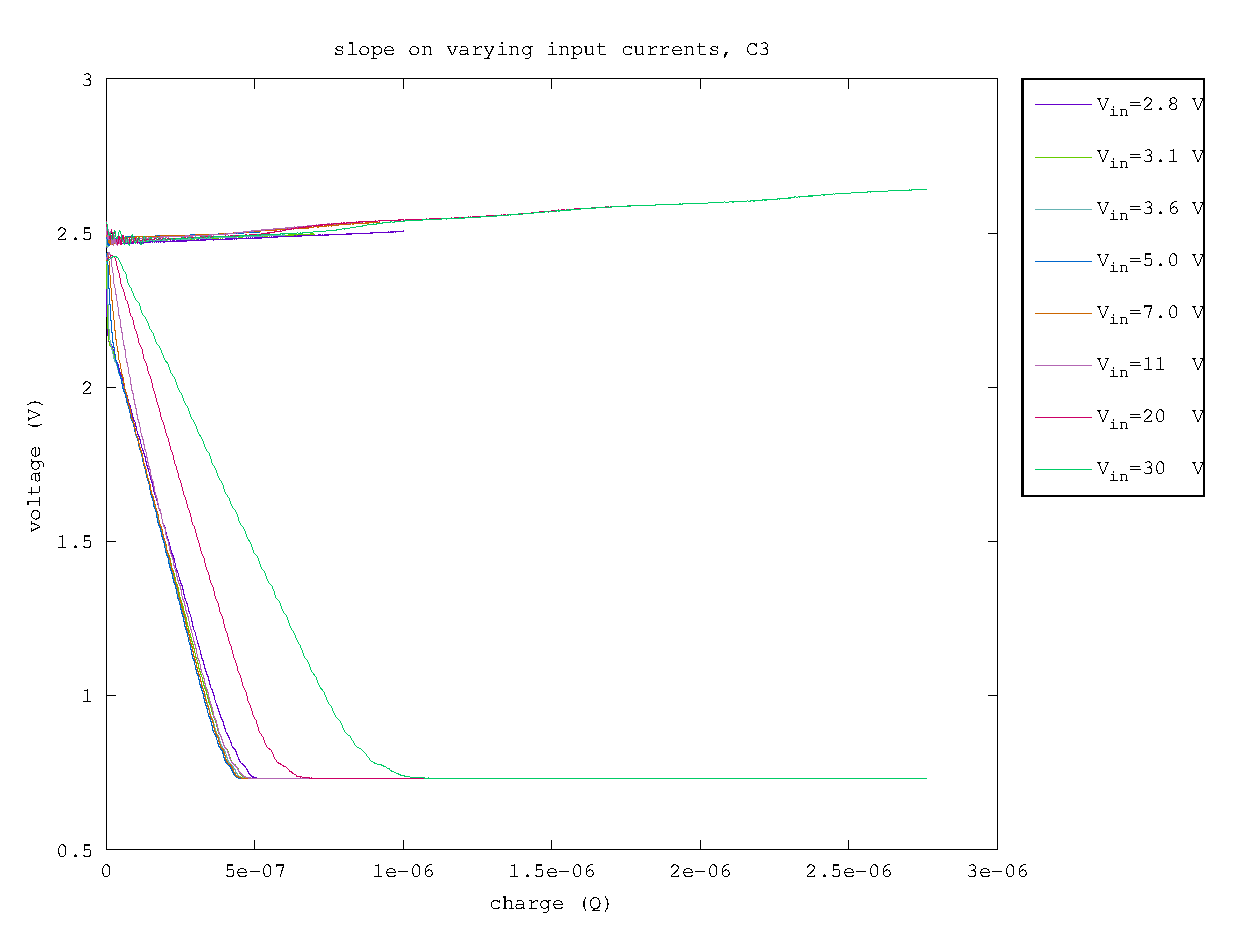
\includegraphics[width=\textwidth]{fig/charge_50fF.eps}
	    \caption[]%
	    {$C=50\,fF$}    
	    \label{fig:charges_50fF}
	\end{subfigure}
	\caption{This plot is showing charge versus voltage}
	\label{fig:charges}
\end{figure}

\Cref{fig:d_slopes} shows the $\delta Q/\delta V$ against charge plots. Note that $\delta Q/\delta V$ is the capacitance. One can observe that while the capacitance is charging, the full value of the capacitancec can be observed, and when the capacitance is comopletely decharged, it behaves as if it is not there. One can use these plots to estimate the integration capacitance. The capitance for \cref{fig:charges_450fF}, \ref{fig:charges_350fF}, \ref{fig:charges_150fF} and \ref{fig:charges_50fF} are approxiately $450\,fF$, $350\,fF$, $220\,fF$ and $180\,fF$ respectively.


\begin{figure}[h]
	\centering
	\begin{subfigure}[b]{0.475\textwidth}
	    \centering
	    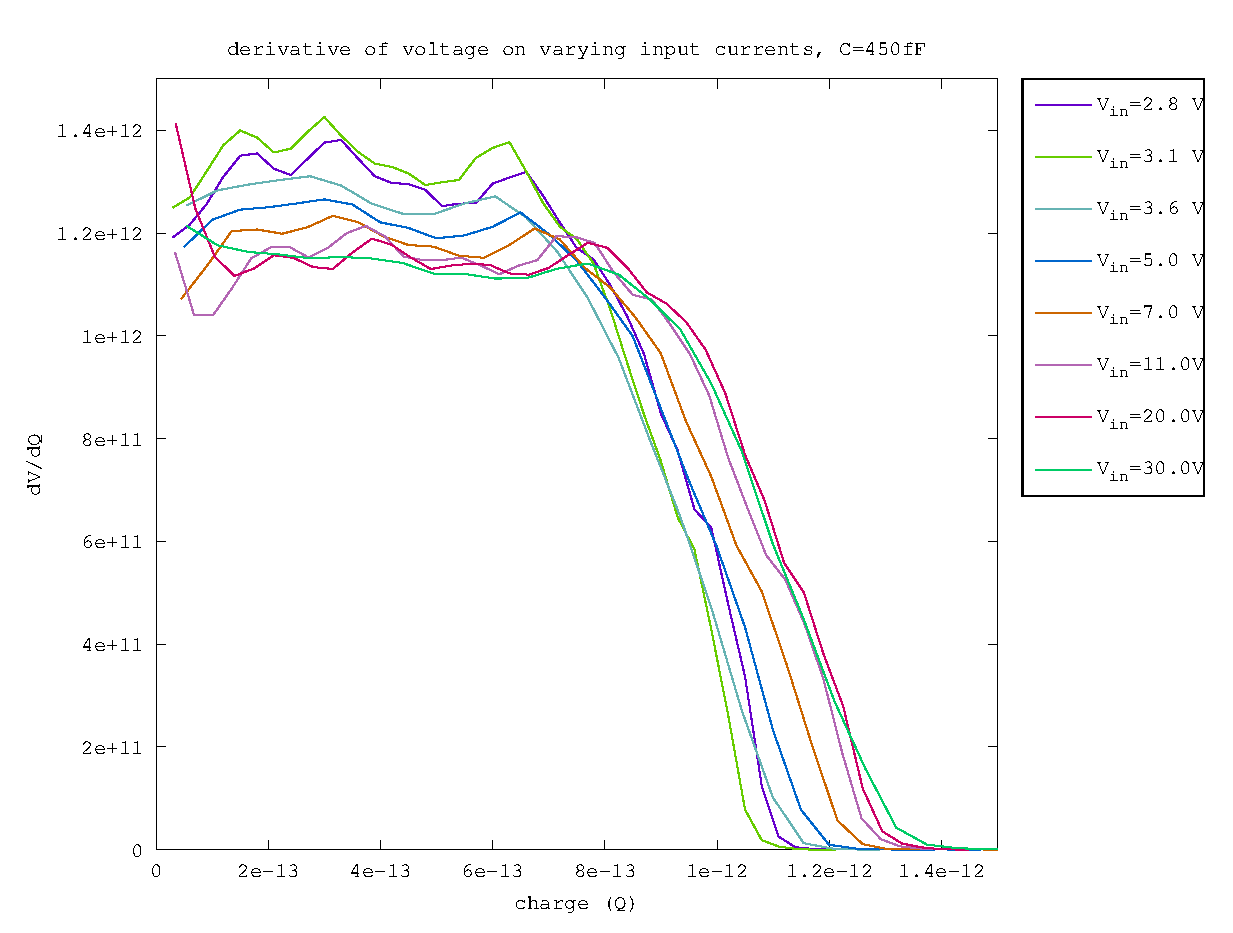
\includegraphics[width=\textwidth]{fig/d_slope_450fF.eps}
	    \caption[Network2]%
	    {$C=450\,fF$}    
	    \label{fig:d_slopes_450fF}
	\end{subfigure}
	\hfill
	\begin{subfigure}[b]{0.475\textwidth}  
	    \centering 
	    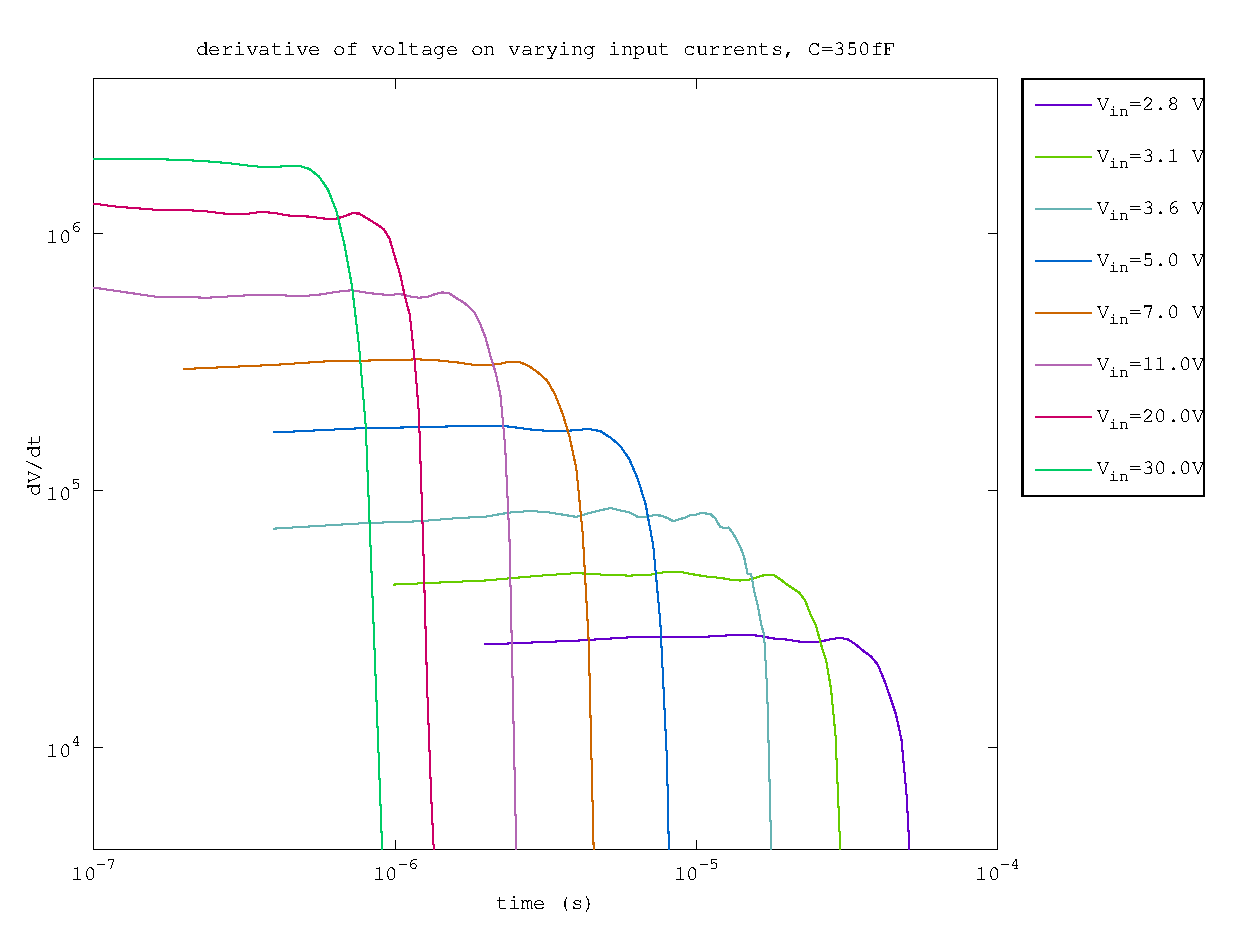
\includegraphics[width=\textwidth]{fig/d_slope_350fF.eps}
	    \caption[]%
	    {$C=350\,fF$}    
	    \label{fig:d_slopes_350fF}
	\end{subfigure}
	\vskip\baselineskip
	\begin{subfigure}[b]{0.475\textwidth}   
	    \centering 
	    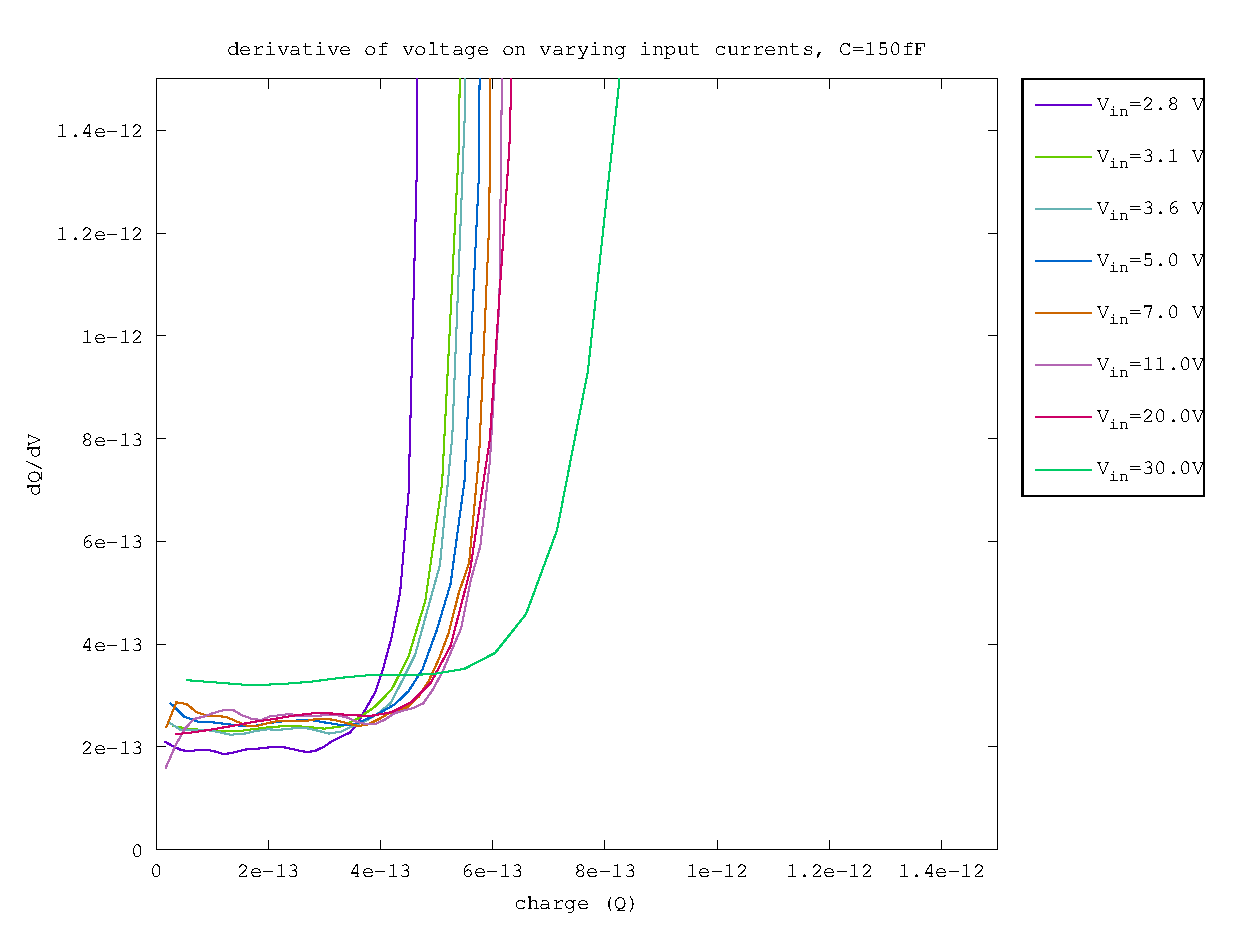
\includegraphics[width=\textwidth]{fig/d_slope_150fF.eps}
	    \caption[]%
	    {$C=150\,fF$}    
	    \label{fig:d_slopes_150fF}
	\end{subfigure}
	\quad
	\begin{subfigure}[b]{0.475\textwidth}   
	    \centering 
	    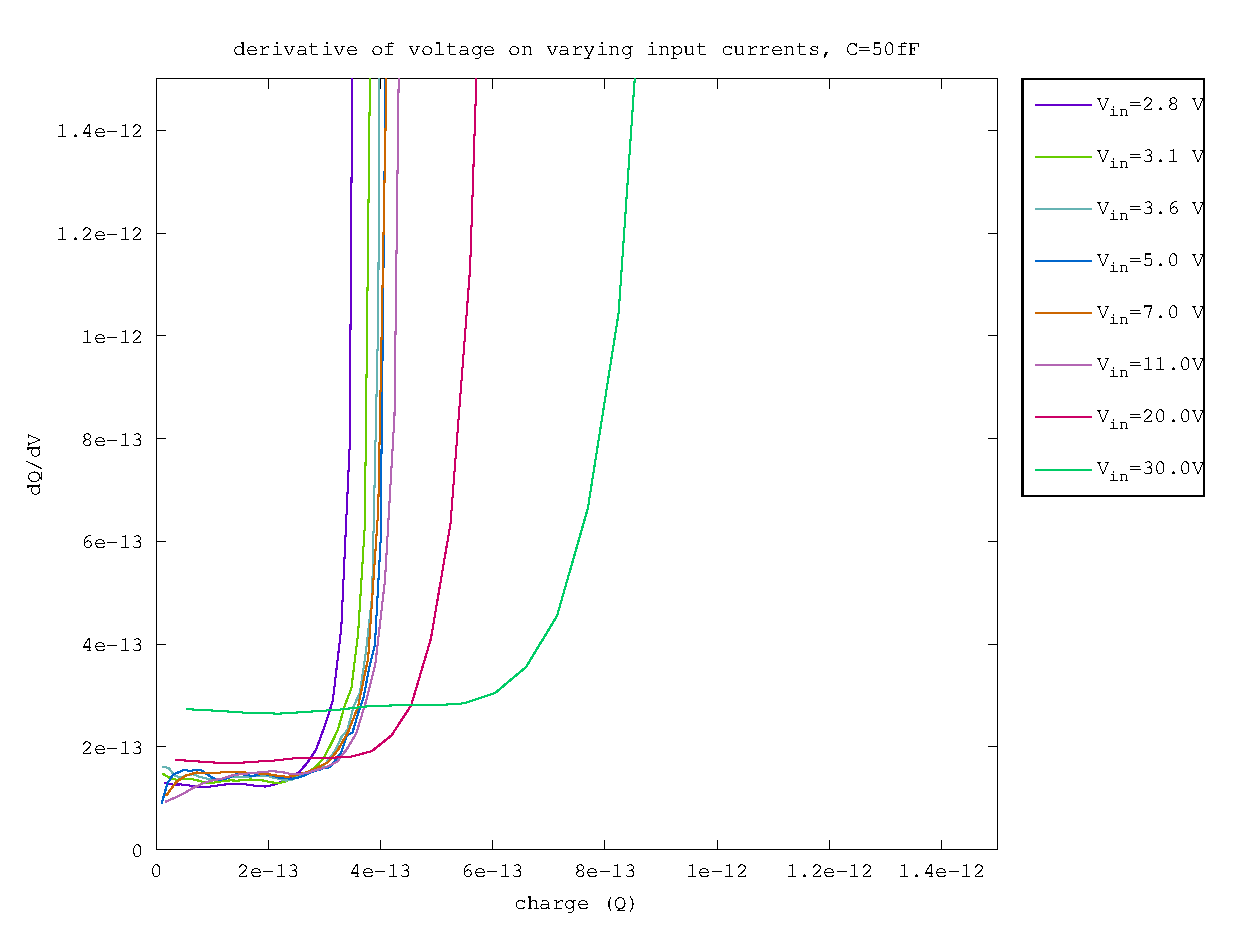
\includegraphics[width=\textwidth]{fig/d_slope_50fF.eps}
	    \caption[]%
	    {$C=50\,fF$}    
	    \label{fig:d_slopes_50fF}
	\end{subfigure}
	\caption{The plot shows dv/dt against time. The plot is in log scale, which allows for an easy read on the maximum slope and the time needed to discharge the integrator capacitance. }
	\label{fig:d_slopes}
\end{figure}



\Cref{fig:e_vs_m} shows $\delta V / \delta t$ against input voltage for all capacitances. One can observe that all four have different slopes at first, but there appears to be a trend that they all converge to a value of $\delta V/\delta t \approx 3.2\cdot10^6$.


\begin{figure}[h]
	    \centering
	    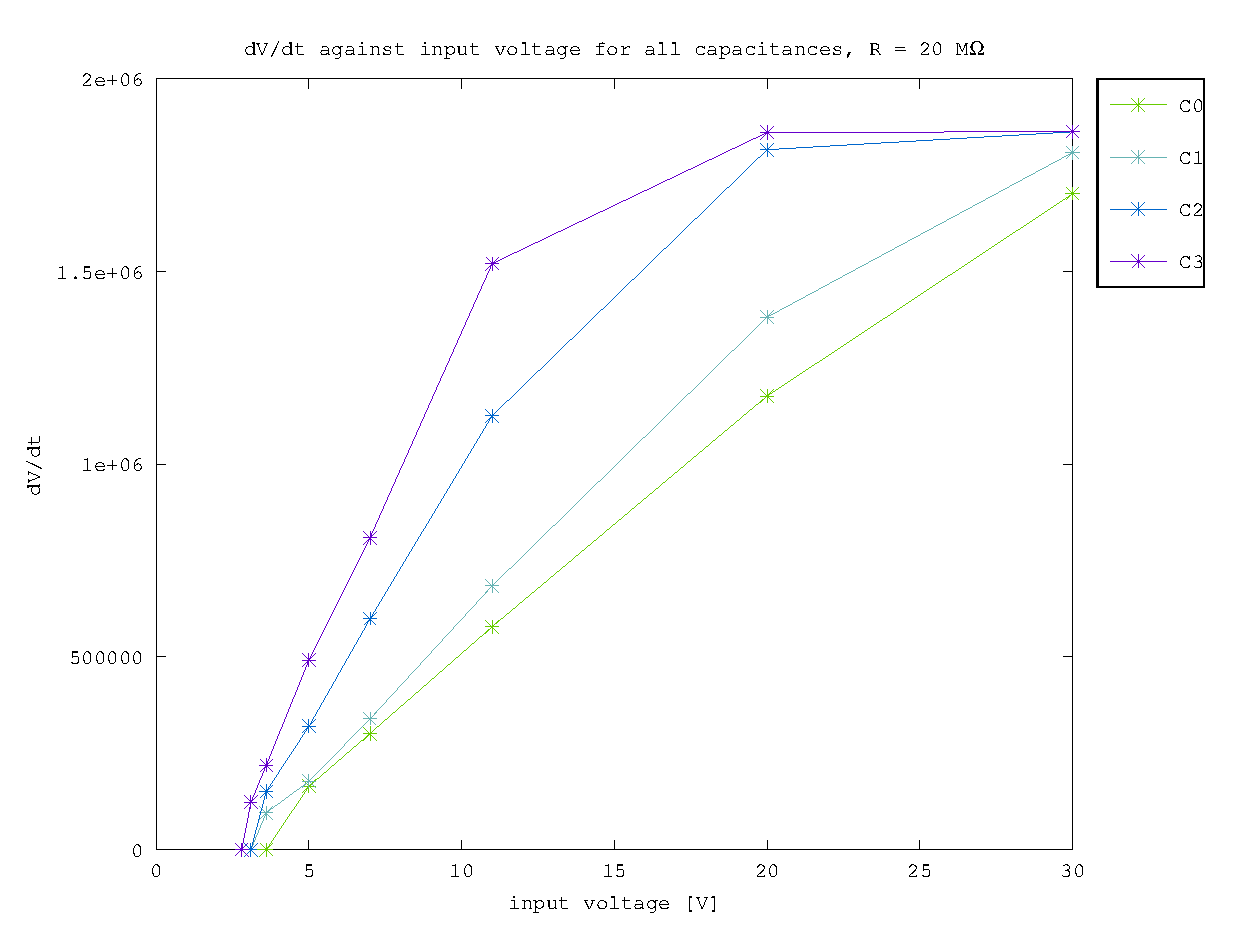
\includegraphics[width=\textwidth]{fig/vin_vs_time_sat.eps}
	    \caption[]%
	    {dV/dt against input voltage for all four capacitances. The x indicate the measurements.}    
	    \label{fig:e_vs_m}	
\end{figure}



\clearpage
\subsection{large current performance}
In this section the $20\,M\Omega$ input resistor is replaecd with a $4\,M\Omega$ resistor. The main goal is to observe the ROIC for very large currents.


\Cref{fig:bre_slopes} shows the same plot as \cref{fig:slopes}, but this time with larger currents. Where a minimum slope could be observed at \cref{fig:slopes}, it is more prevalent here. This also shows more information about the behavior of VBO. For small voltages the VBO does not increase, but as the voltages get larger, one can observe that the voltages of VBO start rising when the OUT is done with decharging. It is also interesting to note that VBO seems to be not affected by the minimum slope at OUT. This gives rise to the hypothesis that the OUT is limited by the source follower. 

\begin{figure}[h]
	\centering
	\begin{subfigure}[b]{0.475\textwidth}
	    \centering
	    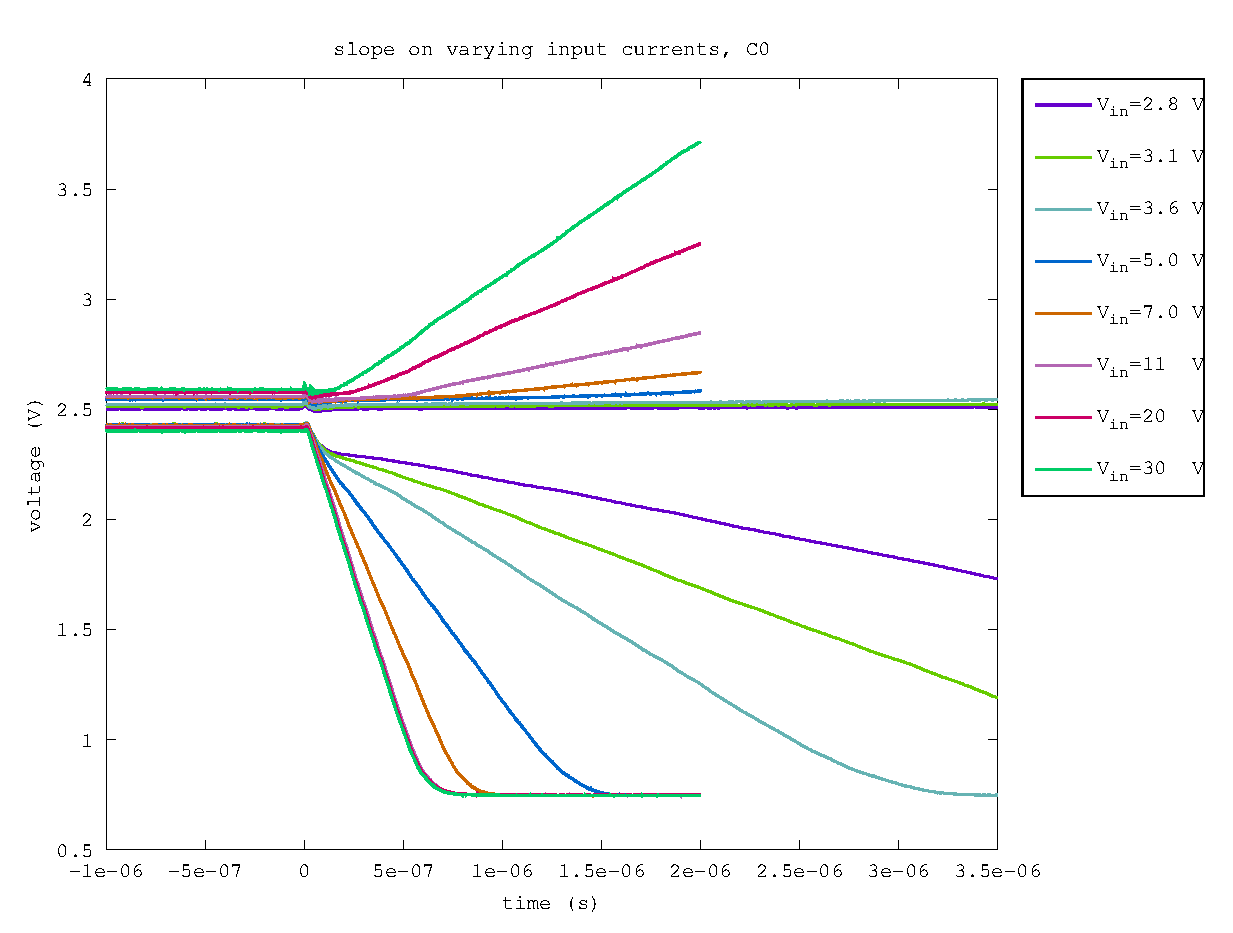
\includegraphics[width=\textwidth]{fig/bre_slope_450fF.eps}
	    \caption[Network2]%
	    {$C=450\,fF$}    
	    \label{fig:bre_slopes_450fF}
	\end{subfigure}
	\hfill
	\begin{subfigure}[b]{0.475\textwidth}  
	    \centering 
	    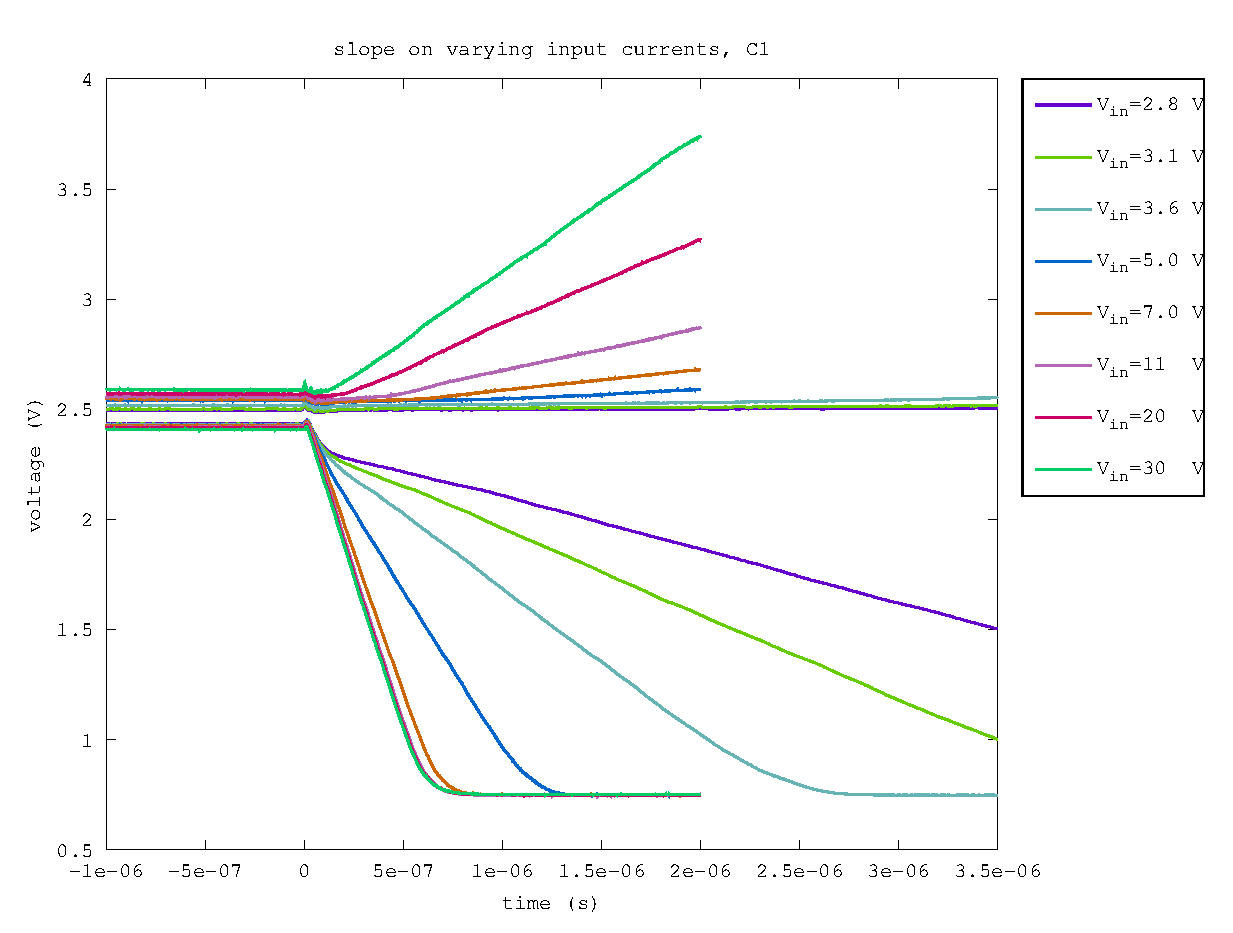
\includegraphics[width=\textwidth]{fig/bre_slope_350fF.eps}
	    \caption[]%
	    {$C=350\,fF$}    
	    \label{fig:bre_slopes_350fF}
	\end{subfigure}
	\vskip\baselineskip
	\begin{subfigure}[b]{0.475\textwidth}   
	    \centering 
	    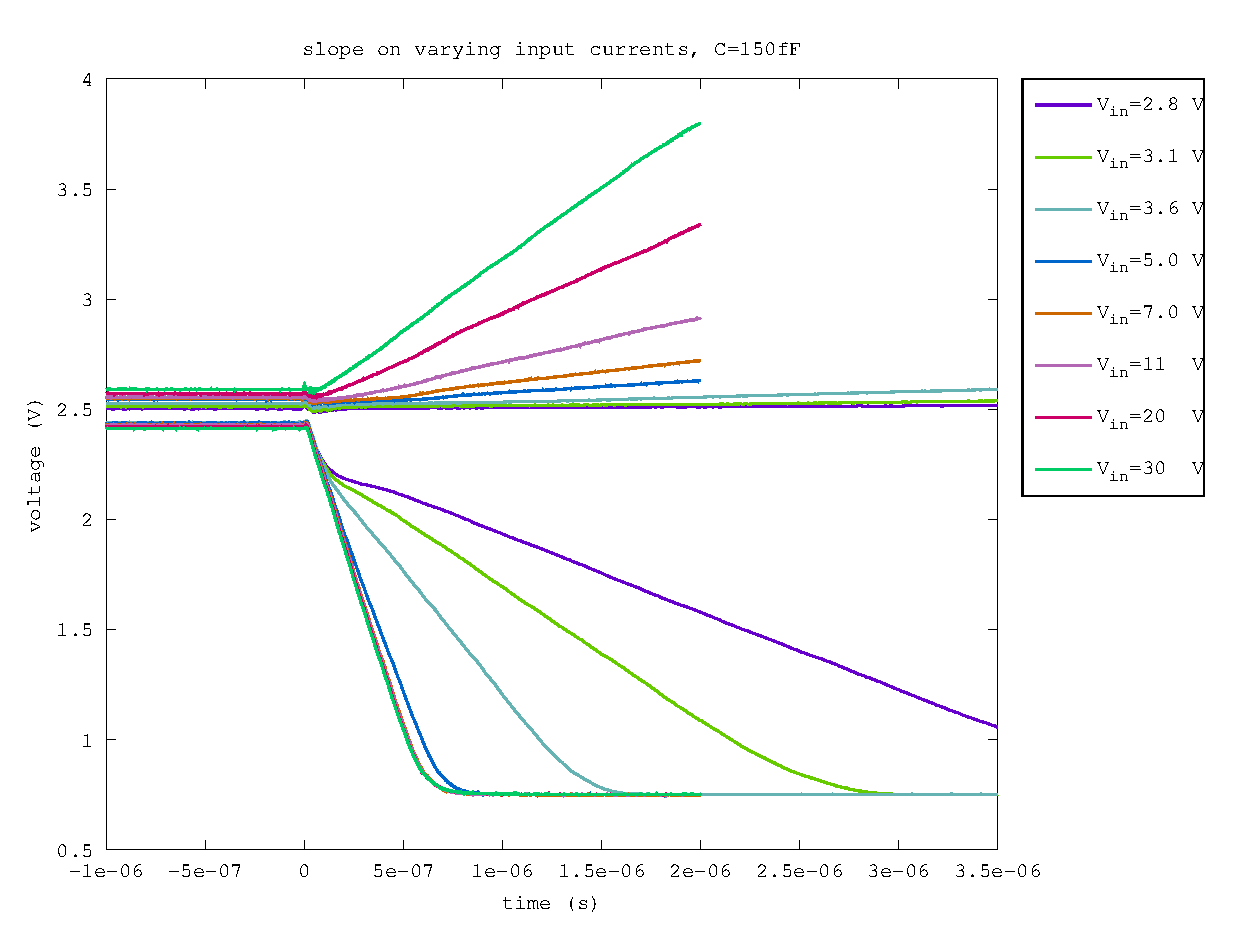
\includegraphics[width=\textwidth]{fig/bre_slope_150fF.eps}
	    \caption[]%
	    {$C=150\,fF$}    
	    \label{fig:bre_slopes_150fF}
	\end{subfigure}
	\quad
	\begin{subfigure}[b]{0.475\textwidth}   
	    \centering 
	    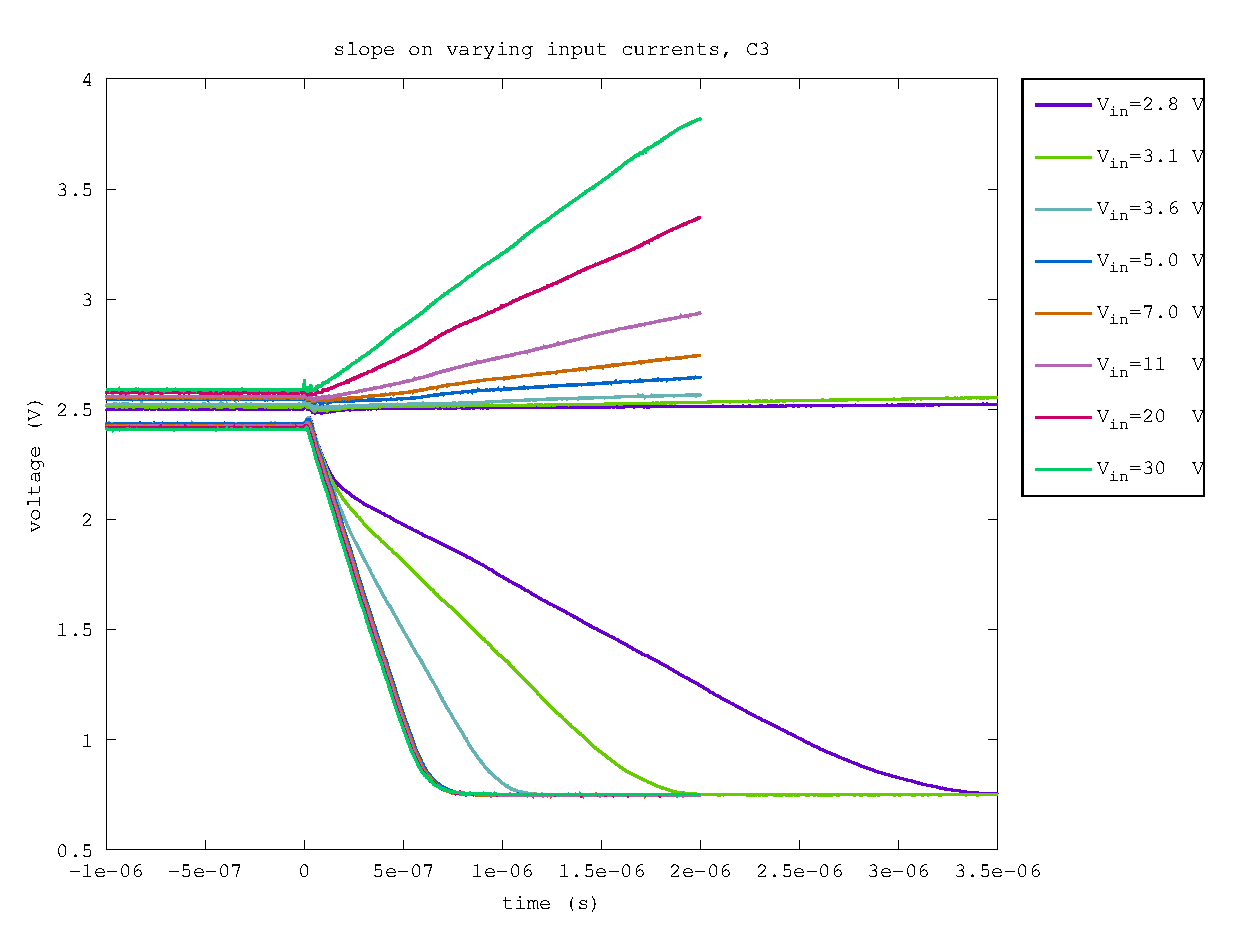
\includegraphics[width=\textwidth]{fig/bre_slope_50fF.eps}
	    \caption[]%
	    {$C=50\,fF$}    
	    \label{fig:bre_slopes_50fF}
	\end{subfigure}
	\caption{Expected versus measured charge up times for different input voltages. The input voltage is connected to the input through a resistor of $4\,M\Omega$}
	\label{fig:bre_slopes}
\end{figure}

\Cref{fig:bre_charges} shows a similar plot as in \cref{fig:charges} but with higher currents. In \cref{fig:charges} one could observe that all currents fitted to the same line, but deviated at higher currents. This effect is also observed here, but in a stronger form. Which is to be expected.

\begin{figure}[h]
	\centering
	\begin{subfigure}[b]{0.475\textwidth}
	    \centering
	    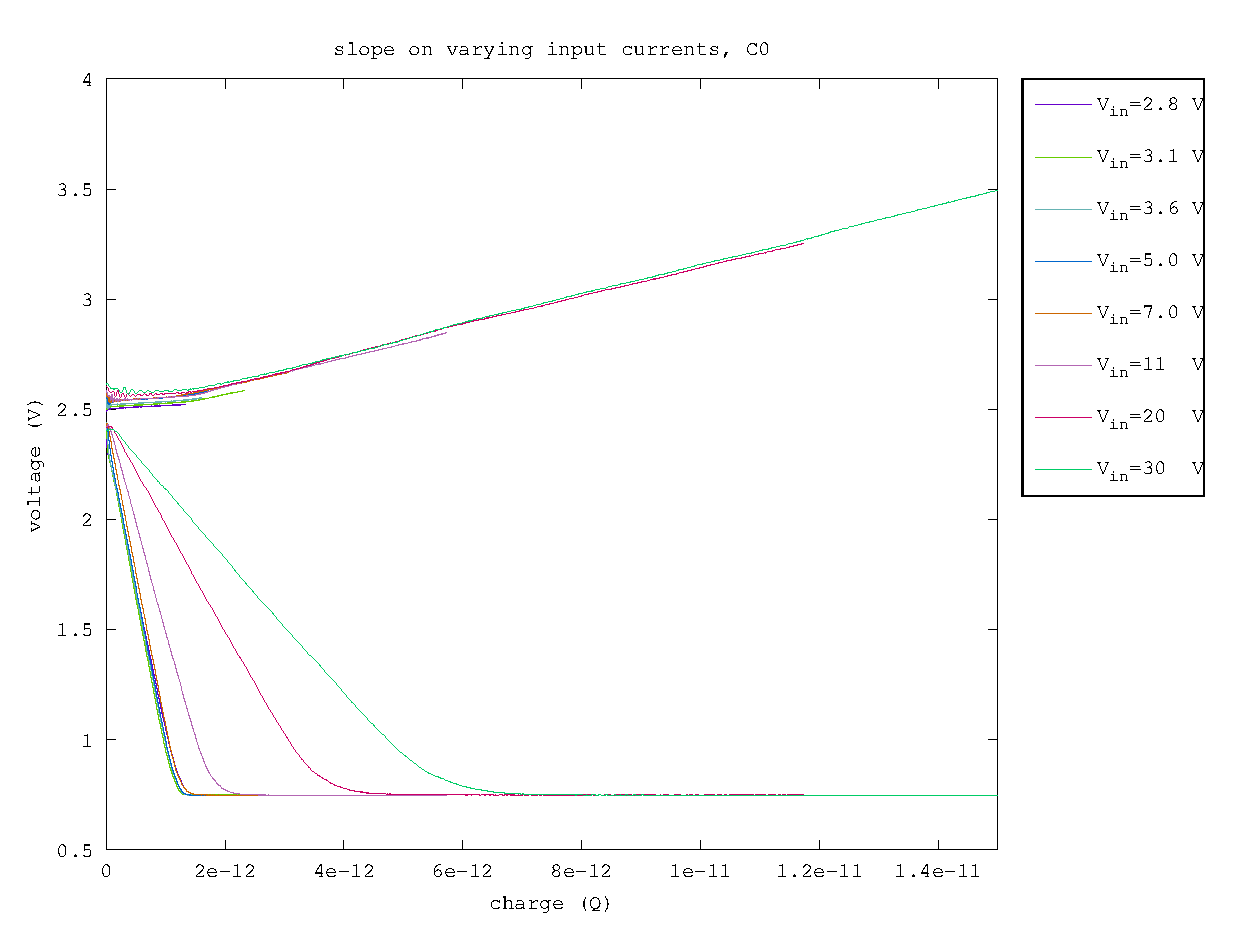
\includegraphics[width=\textwidth]{fig/bre_charge_450fF.eps}
	    \caption[Network2]%
	    {$C=450\,fF$}    
	    \label{fig:bre_charges_450fF}
	\end{subfigure}
	\hfill
	\begin{subfigure}[b]{0.475\textwidth}  
	    \centering 
	    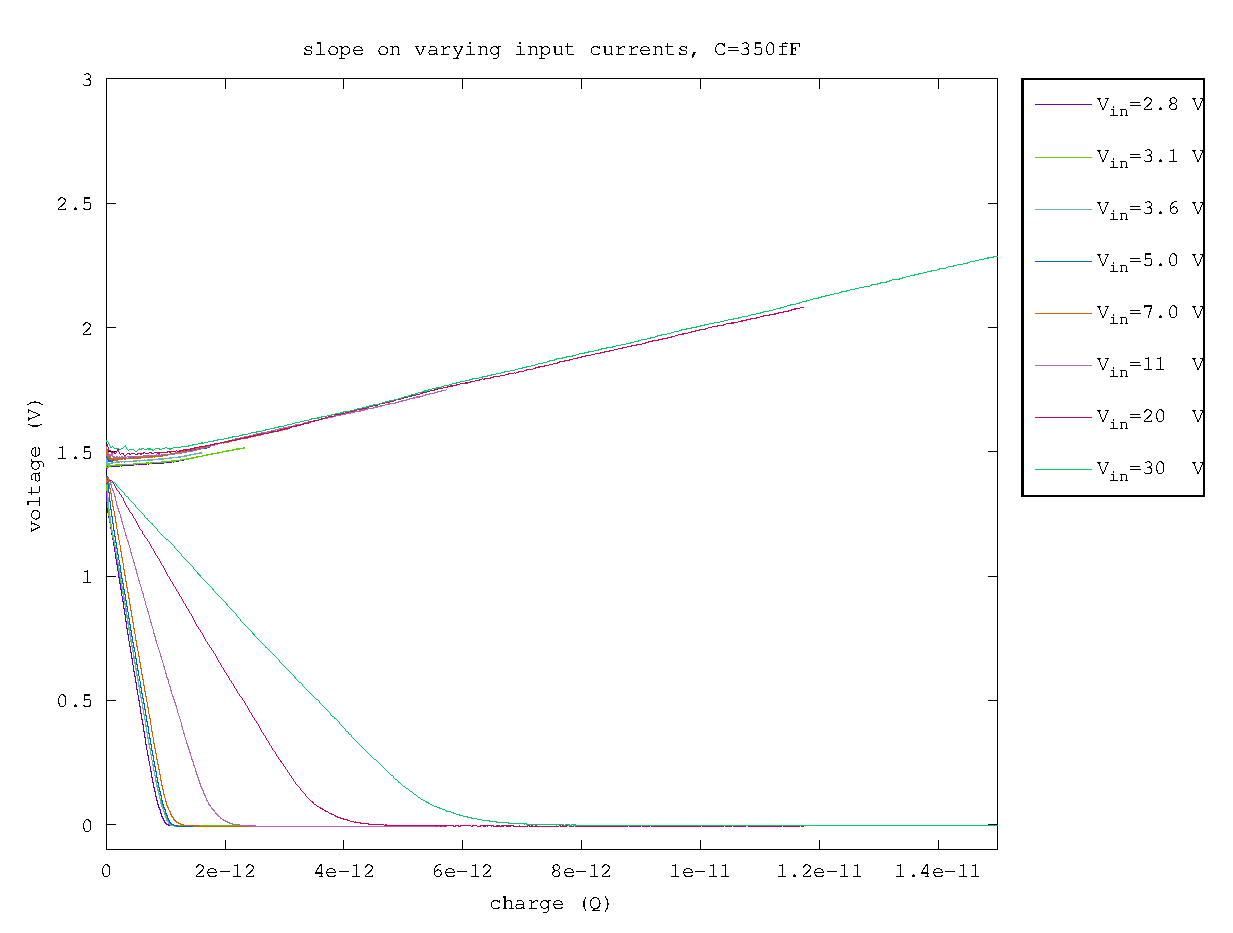
\includegraphics[width=\textwidth]{fig/bre_charge_350fF.eps}
	    \caption[]%
	    {$C=350\,fF$}    
	    \label{fig:bre_charges_350fF}
	\end{subfigure}
	\vskip\baselineskip
	\begin{subfigure}[b]{0.475\textwidth}   
	    \centering 
	    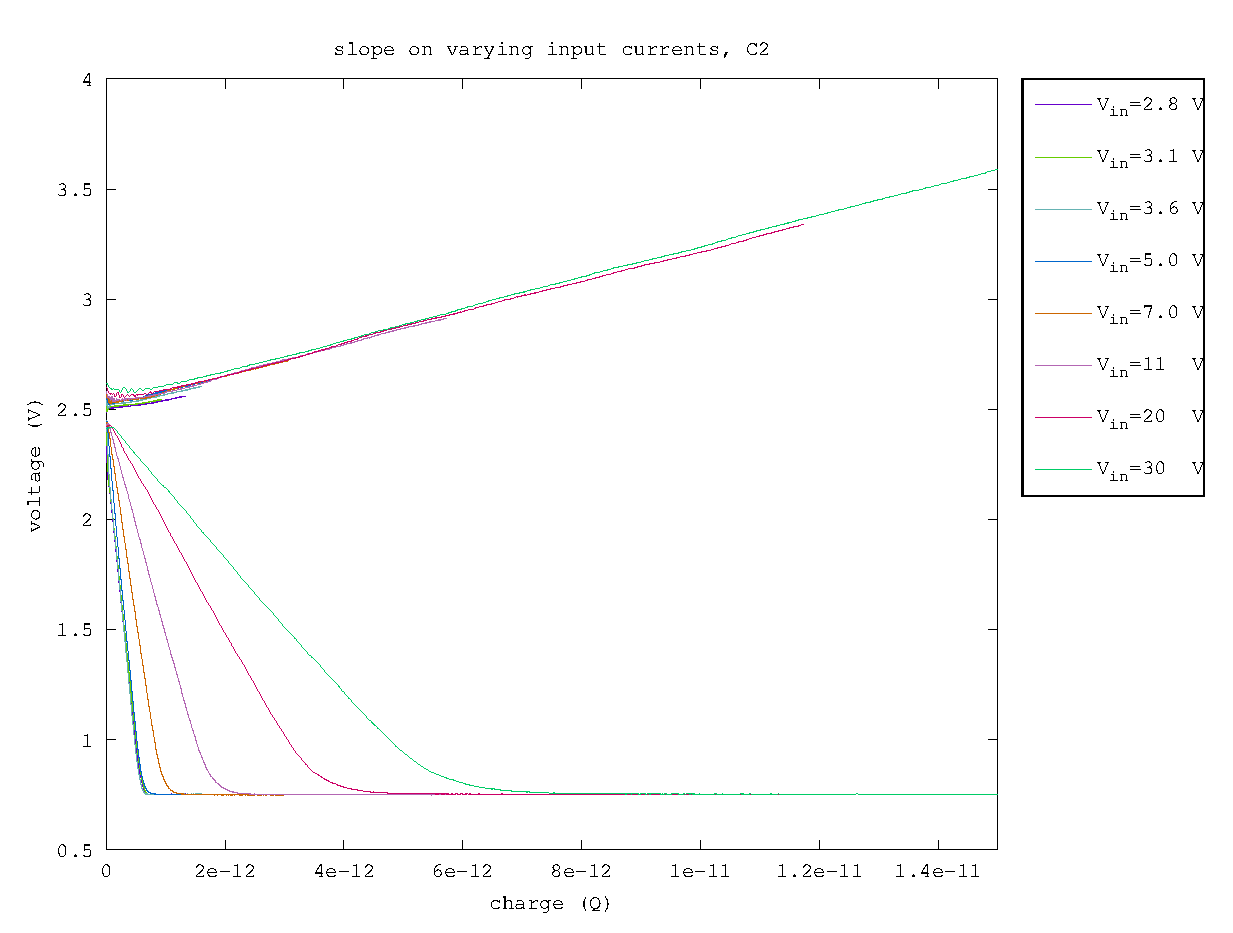
\includegraphics[width=\textwidth]{fig/bre_charge_150fF.eps}
	    \caption[]%
	    {$C=150\,fF$}    
	    \label{fig:bre_charges_150fF}
	\end{subfigure}
	\quad
	\begin{subfigure}[b]{0.475\textwidth}   
	    \centering 
	    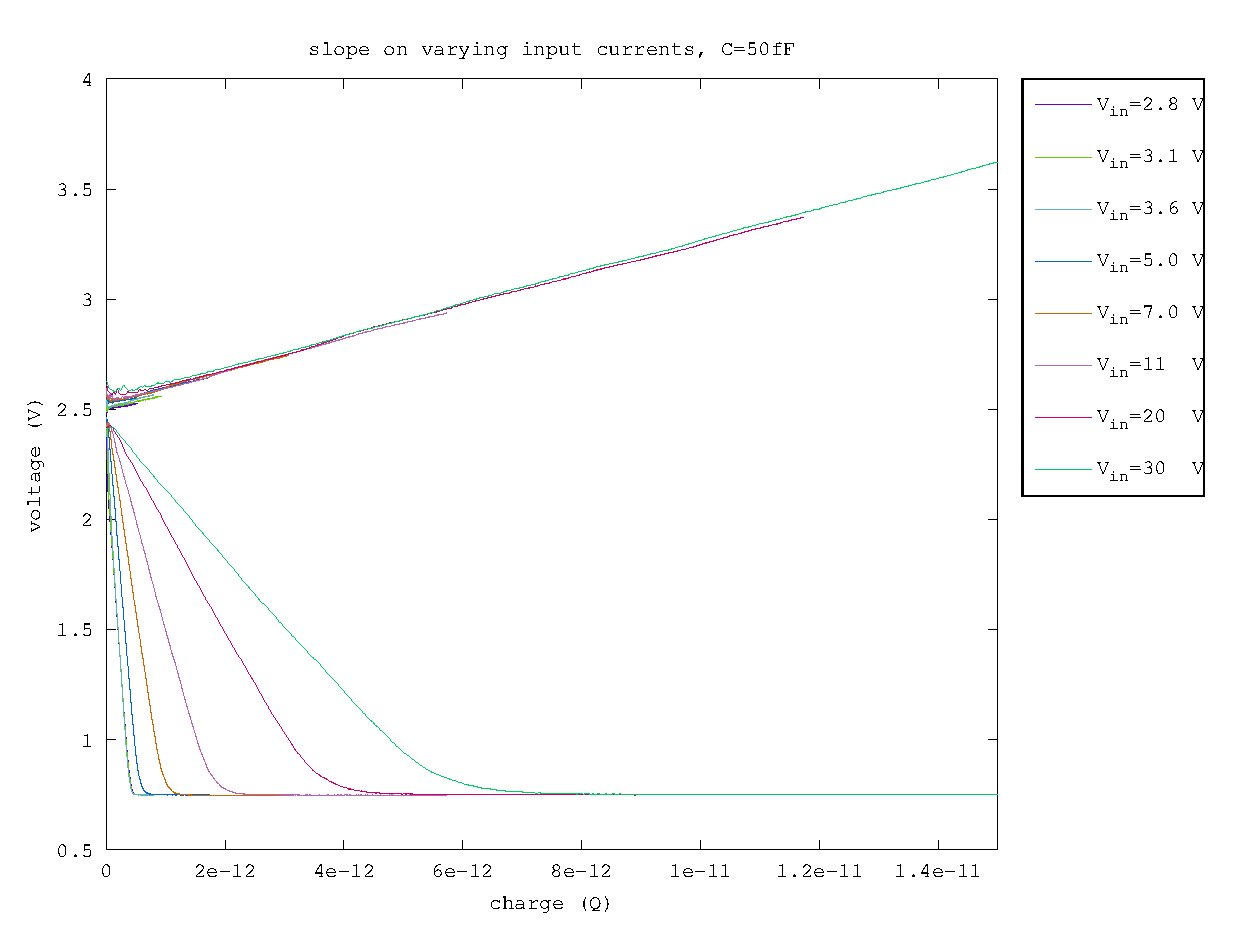
\includegraphics[width=\textwidth]{fig/bre_charge_50fF.eps}
	    \caption[]%
	    {$C=50\,fF$}    
	    \label{fig:bre_charges_50fF}
	\end{subfigure}
	\caption{This plot is showing charge versus voltage}
	\label{fig:bre_charges}
\end{figure}

\Cref{fig:bre_d_slopes} shows a plot of $\delta V/\delta Q$ against charge. Note that the behavior for the low voltages differ across the different capacitances, but that the high voltages are not affected by a change in capacitance. This observation agrees with the hypothesis that the output is not limited by the input current, but by the speed of the source follower at the output.

\begin{figure}[h]
	\centering
	\begin{subfigure}[b]{0.475\textwidth}
	    \centering
	    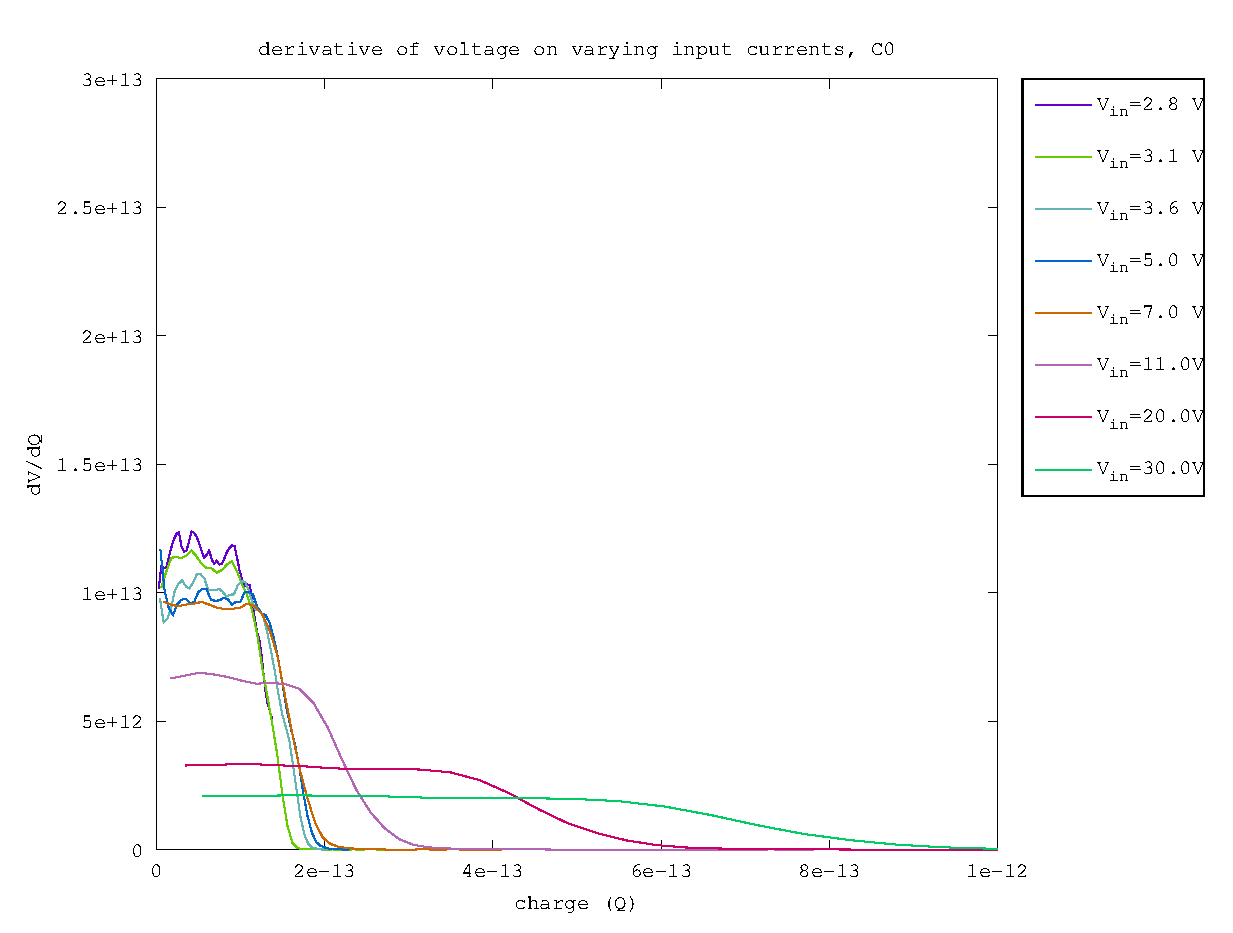
\includegraphics[width=\textwidth]{fig/bre_d_slope_450fF.eps}
	    \caption[Network2]%
	    {$C=450\,fF$}    
	    \label{fig:bre_d_slopes_450fF}
	\end{subfigure}
	\hfill
	\begin{subfigure}[b]{0.475\textwidth}  
	    \centering 
	    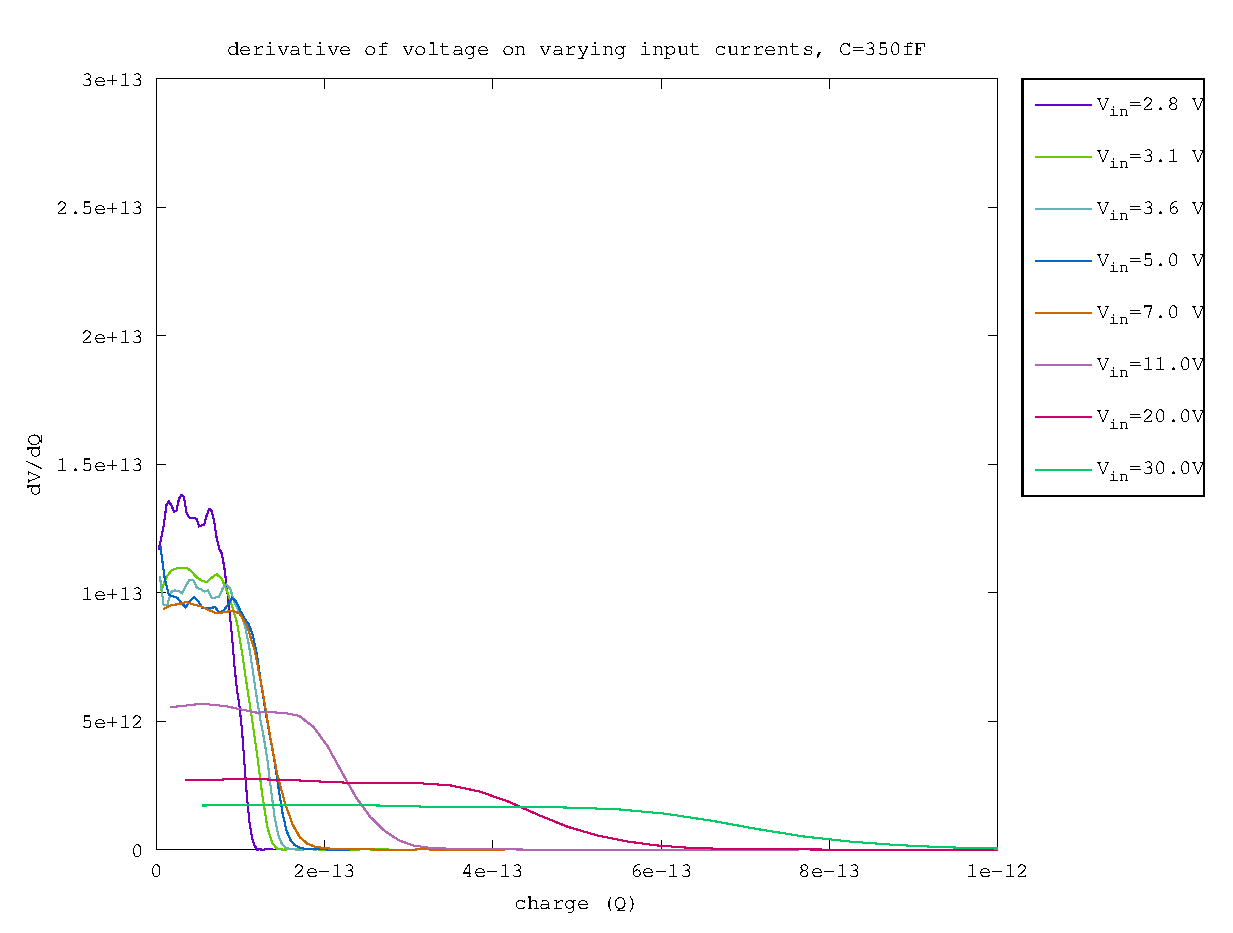
\includegraphics[width=\textwidth]{fig/bre_d_slope_350fF.eps}
	    \caption[]%
	    {$C=350\,fF$}    
	    \label{fig:bre_d_slopes_350fF}
	\end{subfigure}
	\vskip\baselineskip
	\begin{subfigure}[b]{0.475\textwidth}   
	    \centering 
	    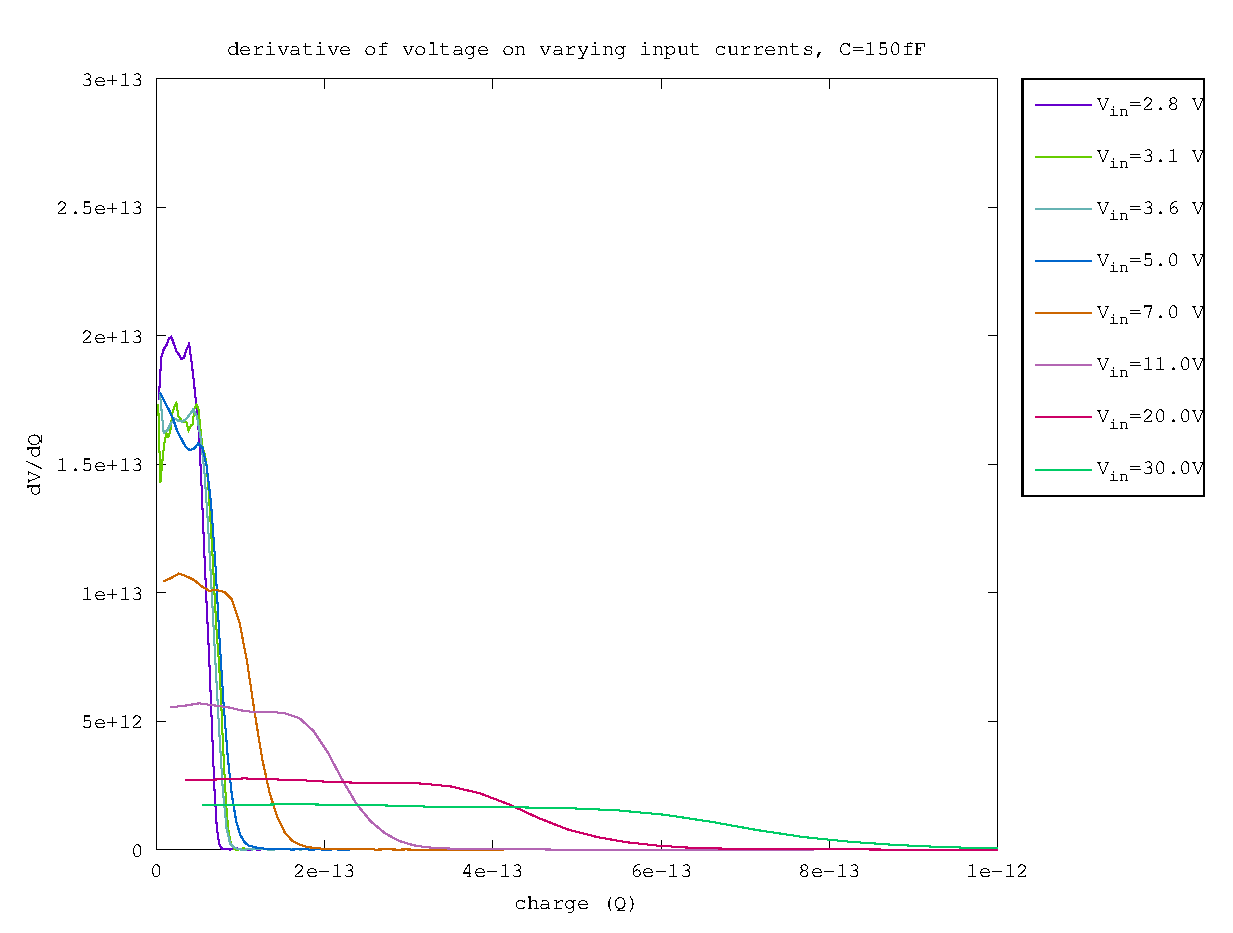
\includegraphics[width=\textwidth]{fig/bre_d_slope_150fF.eps}
	    \caption[]%
	    {$C=150\,fF$}    
	    \label{fig:bre_d_slopes_150fF}
	\end{subfigure}
	\quad
	\begin{subfigure}[b]{0.475\textwidth}   
	    \centering 
	    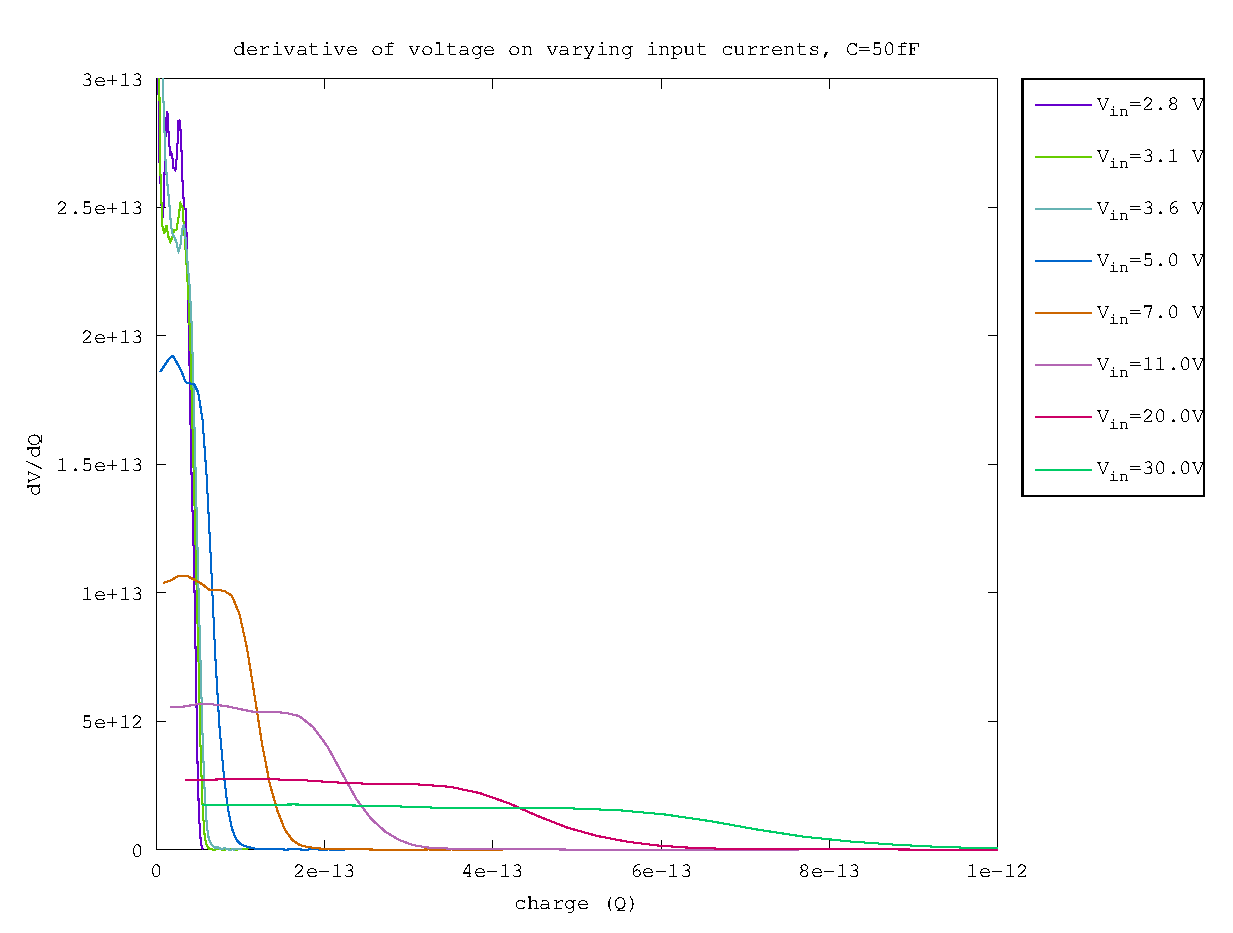
\includegraphics[width=\textwidth]{fig/bre_d_slope_50fF.eps}
	    \caption[]%
	    {$C=50\,fF$}    
	    \label{fig:bre_d_slopes_50fF}
	\end{subfigure}
	\caption{The plot shows dv/dt against time. The plot is in log scale, which allows for an easy read on the maximum slope and the time needed to discharge the integrator capacitance. }
	\label{fig:bre_d_slopes}
\end{figure}

\Cref{fig:bre_e_vs_m} shows the same plot as \cref{fig:e_vs_m}, but with higher current. This plot clearly shows that all four capacitance configurations saturate at a $\delta V\delta t \approx 3.1\,V$. This cannot be a limit applied to the input, because the capacitances are different. Therefore the output is limiting this, conform previous observations.

\begin{figure}[h]
	    \centering
	    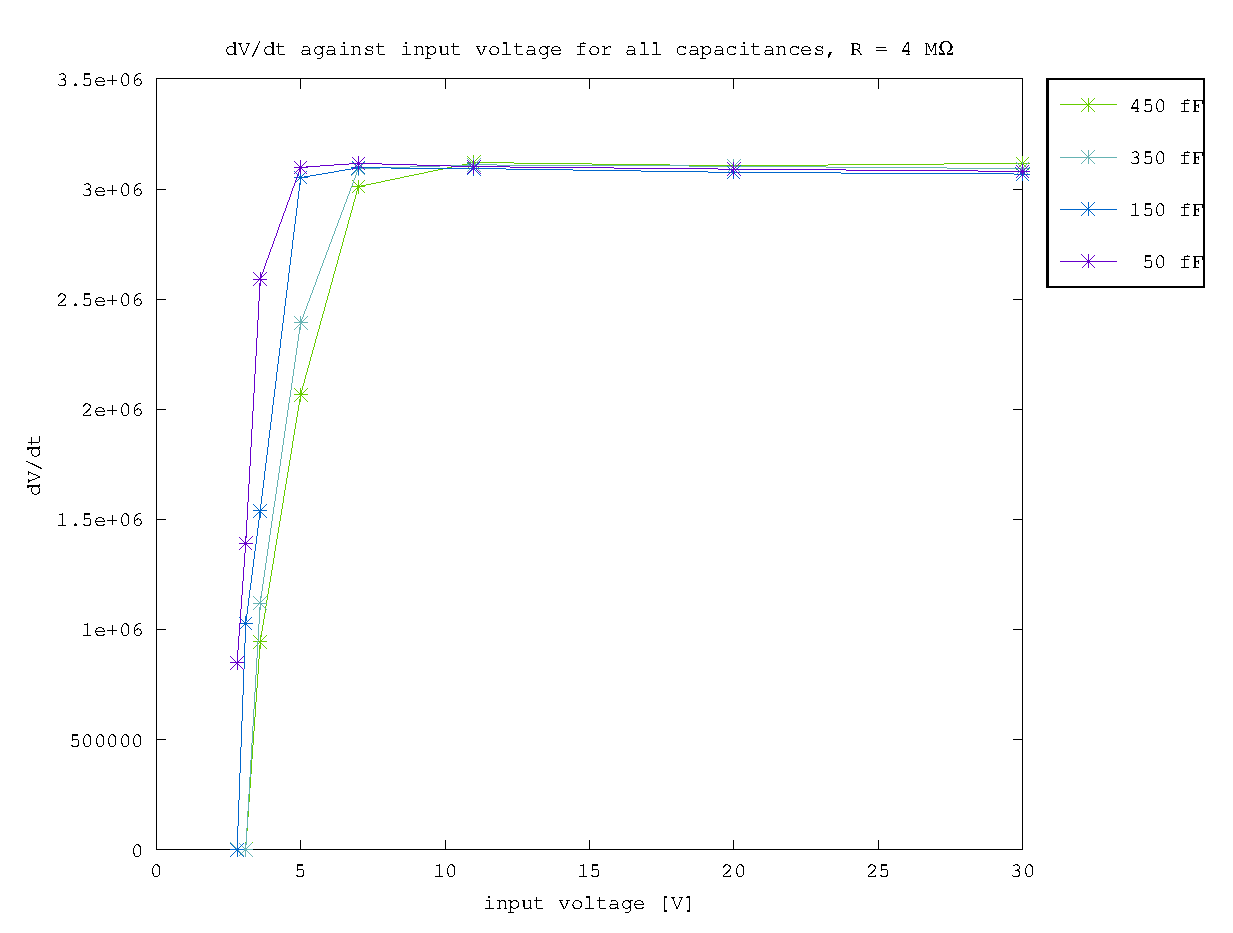
\includegraphics[width=\textwidth]{fig/bre_vin_vs_time_sat.eps}
	    \caption[]%
	    {dV/dt against input voltage for all four capacitances. The x indicate the measurements.}    
	    \label{fig:bre_e_vs_m}	
\end{figure}

\clearpage
\subsection{Voltage limiter}
This section focusses on the output of the source follower that is directly connected to the output of the high voltage transistor connected to the input of the ROIC. The setup is identical to \cref{ssec:standard}, but the time scale is different to oberve the slower behavior of VBO.

\Cref{fig:vbo_slopes} shows the time against voltage plot. This are a couple of important observations that can be made from these plots. First and foremost: the behavior ofthe VBO is almost not affected by the capacitance. The behavior is fairly similar. There is a difference however, in that the VBO starts rising as the OUT reaches zero. This means that the VBO for $450\,fF$ is slightly delayed when compared to $50\,fF$ for example. It is also intersting yo observe that VBO never increases above $2.6\,V$. This behavior is most likely due to the high voltage input transistor doing it's job as a current limiter. Finally one can observe that for very low currents, VBO does not reach $2.6\,V$. The reason for this is that the input reaches the voltage level of the power supply before the current limiter kicks in.


\begin{figure}[h]
	\centering
	\begin{subfigure}[b]{0.475\textwidth}
	    \centering
	    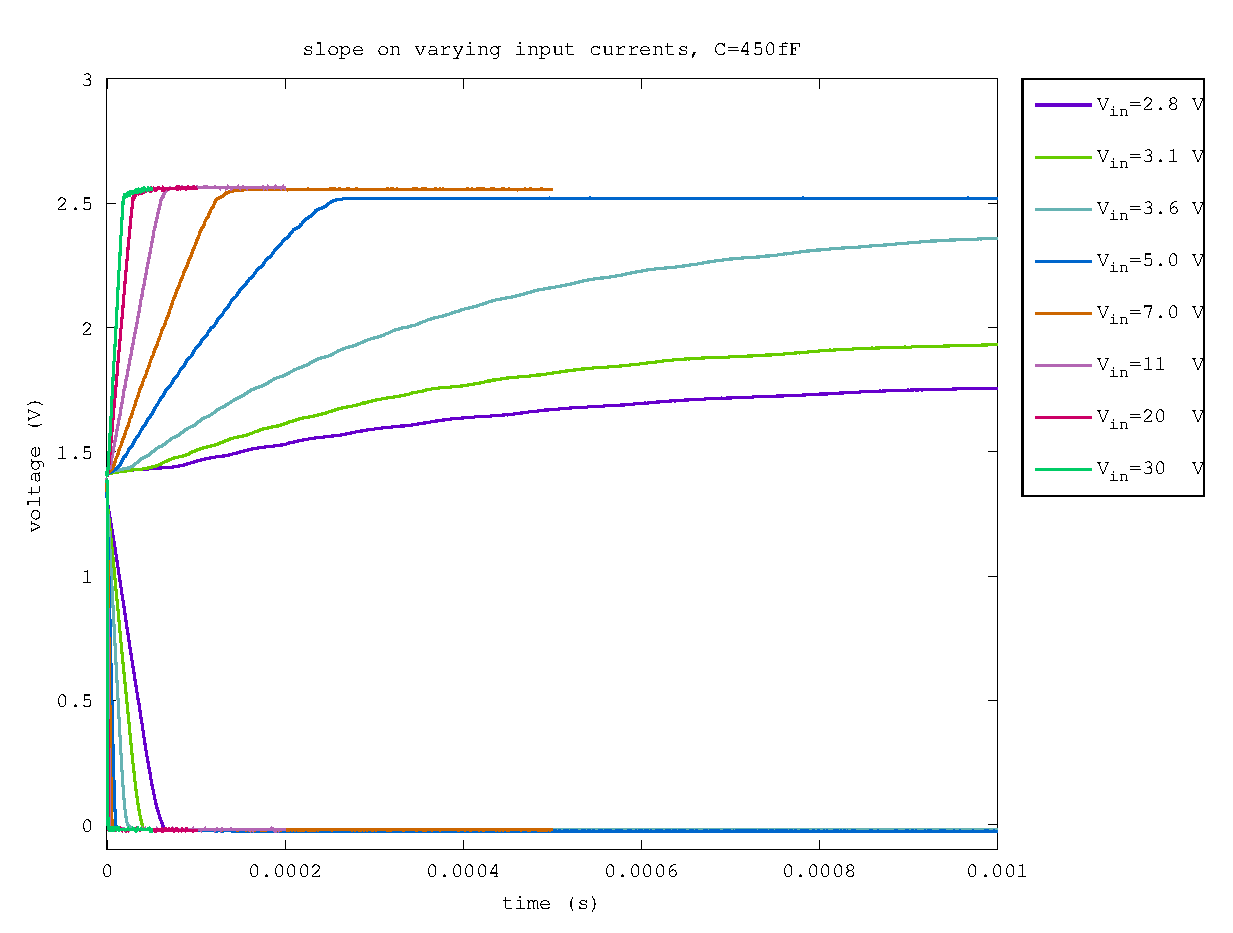
\includegraphics[width=\textwidth]{fig/vbo_slope_450fF.eps}
	    \caption[Network2]%
	    {$C=450\,fF$}    
	    \label{fig:vbo_slopes_450fF}
	\end{subfigure}
	\hfill
	\begin{subfigure}[b]{0.475\textwidth}  
	    \centering 
	    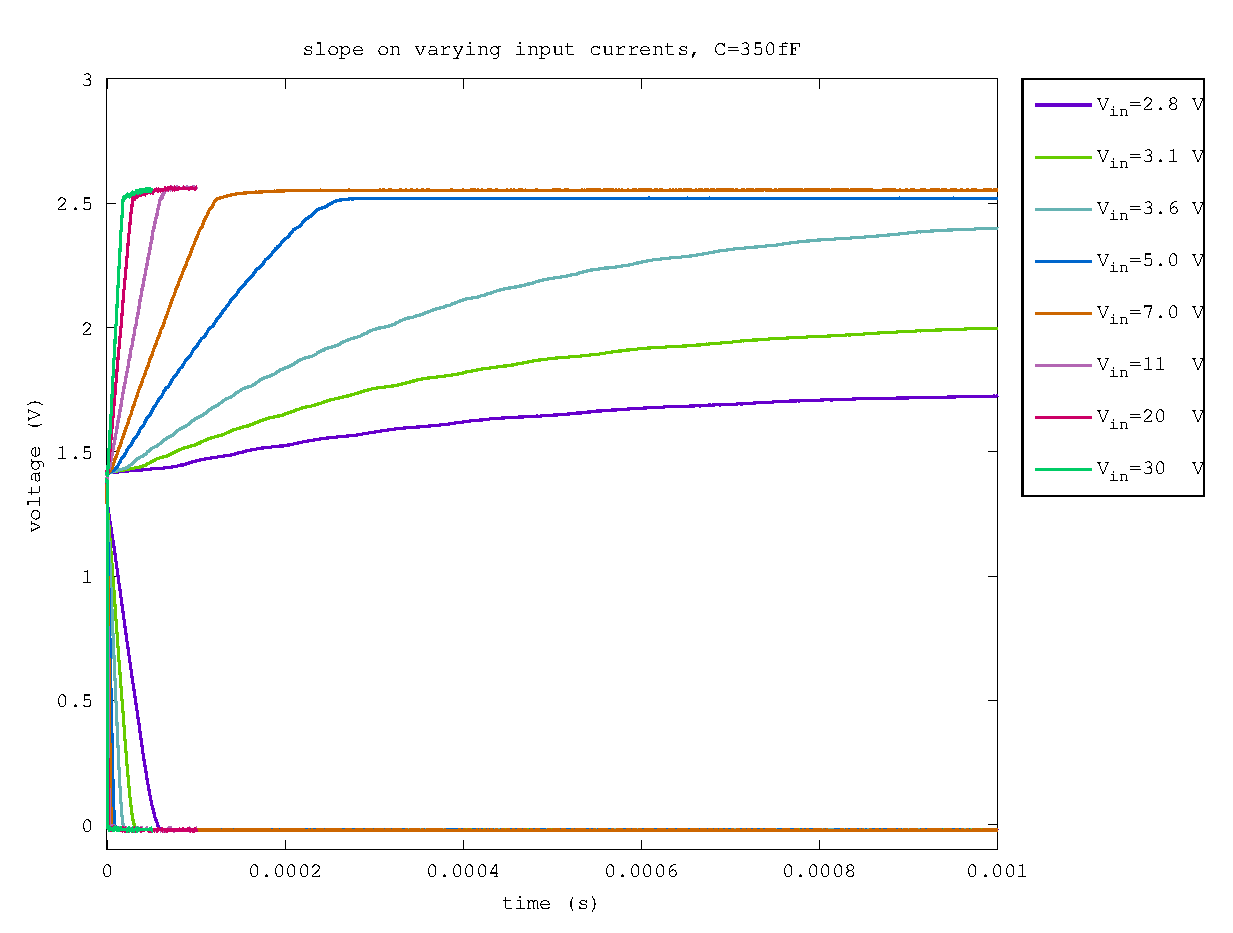
\includegraphics[width=\textwidth]{fig/vbo_slope_350fF.eps}
	    \caption[]%
	    {$C=350\,fF$}    
	    \label{fig:vbo_slopes_350fF}
	\end{subfigure}
	\vskip\baselineskip
	\begin{subfigure}[b]{0.475\textwidth}   
	    \centering 
	    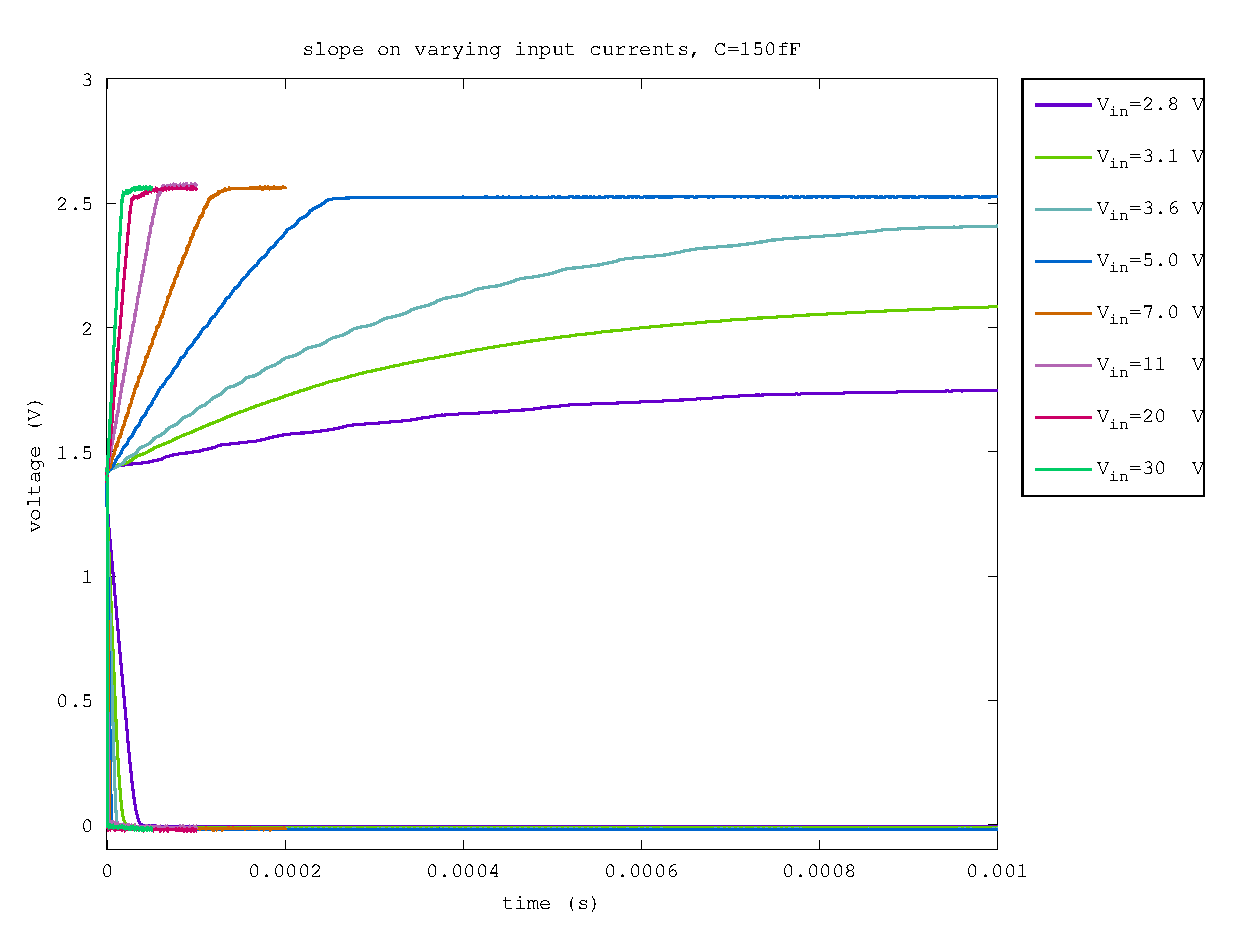
\includegraphics[width=\textwidth]{fig/vbo_slope_150fF.eps}
	    \caption[]%
	    {$C=150\,fF$}    
	    \label{fig:vbo_slopes_150fF}
	\end{subfigure}
	\quad
	\begin{subfigure}[b]{0.475\textwidth}   
	    \centering 
	    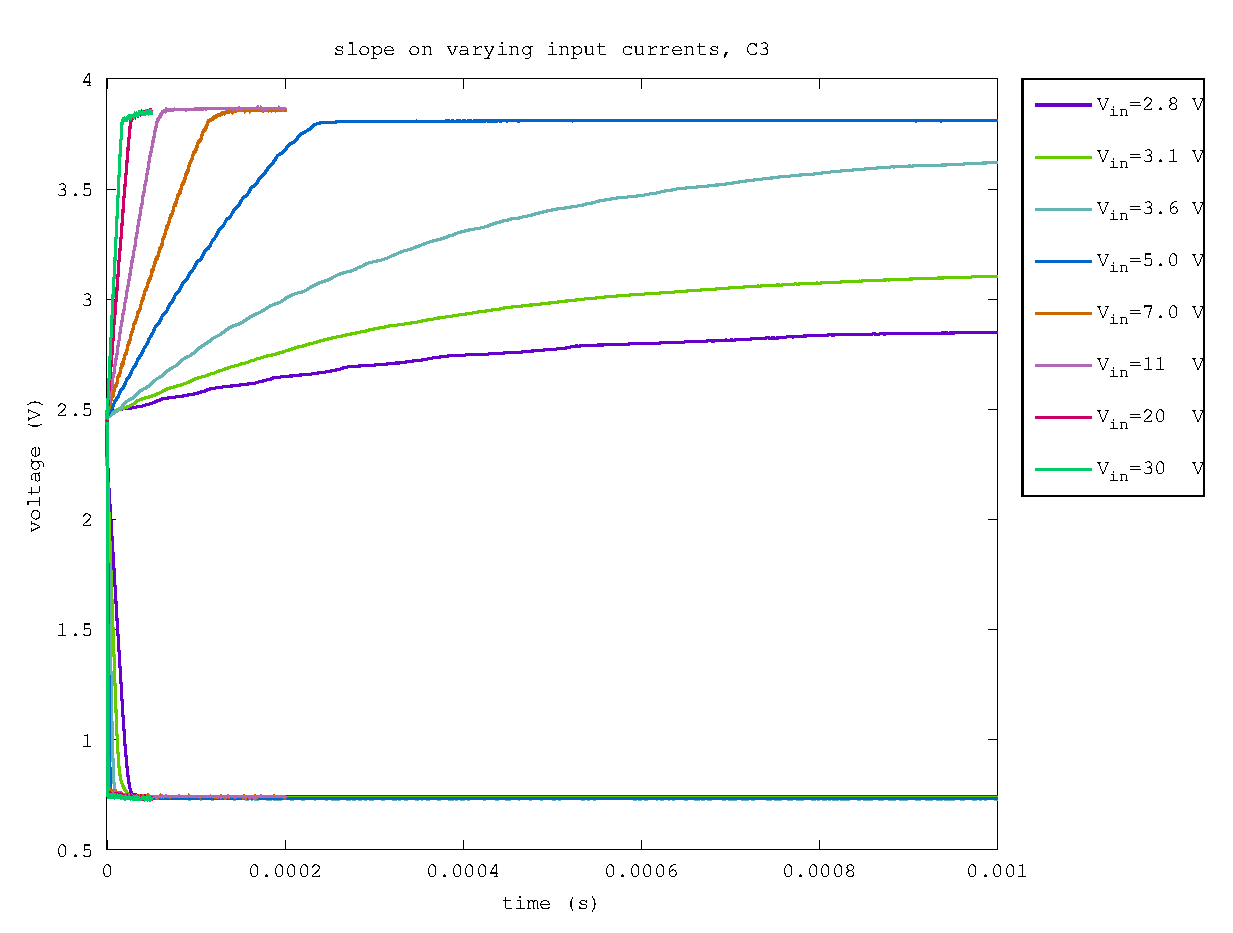
\includegraphics[width=\textwidth]{fig/vbo_slope_50fF.eps}
	    \caption[]%
	    {$C=50\,fF$}    
	    \label{fig:vbo_slopes_50fF}
	\end{subfigure}
	\caption{Expected versus measured charge up times for different input voltages. The input voltage is connected to the input through a resistor of $20\,M\Omega$}
	\label{fig:vbo_slopes}
\end{figure}

\Cref{fig:vbo_charges} shows the plots of voltage against charge. One can observe that increasing the current causes the behavior to converge to a line with a linear slope that is constant with Q, and a saturation at $2.6\,V$. 

\begin{figure}[h]
	\centering
	\begin{subfigure}[b]{0.475\textwidth}
	    \centering
	    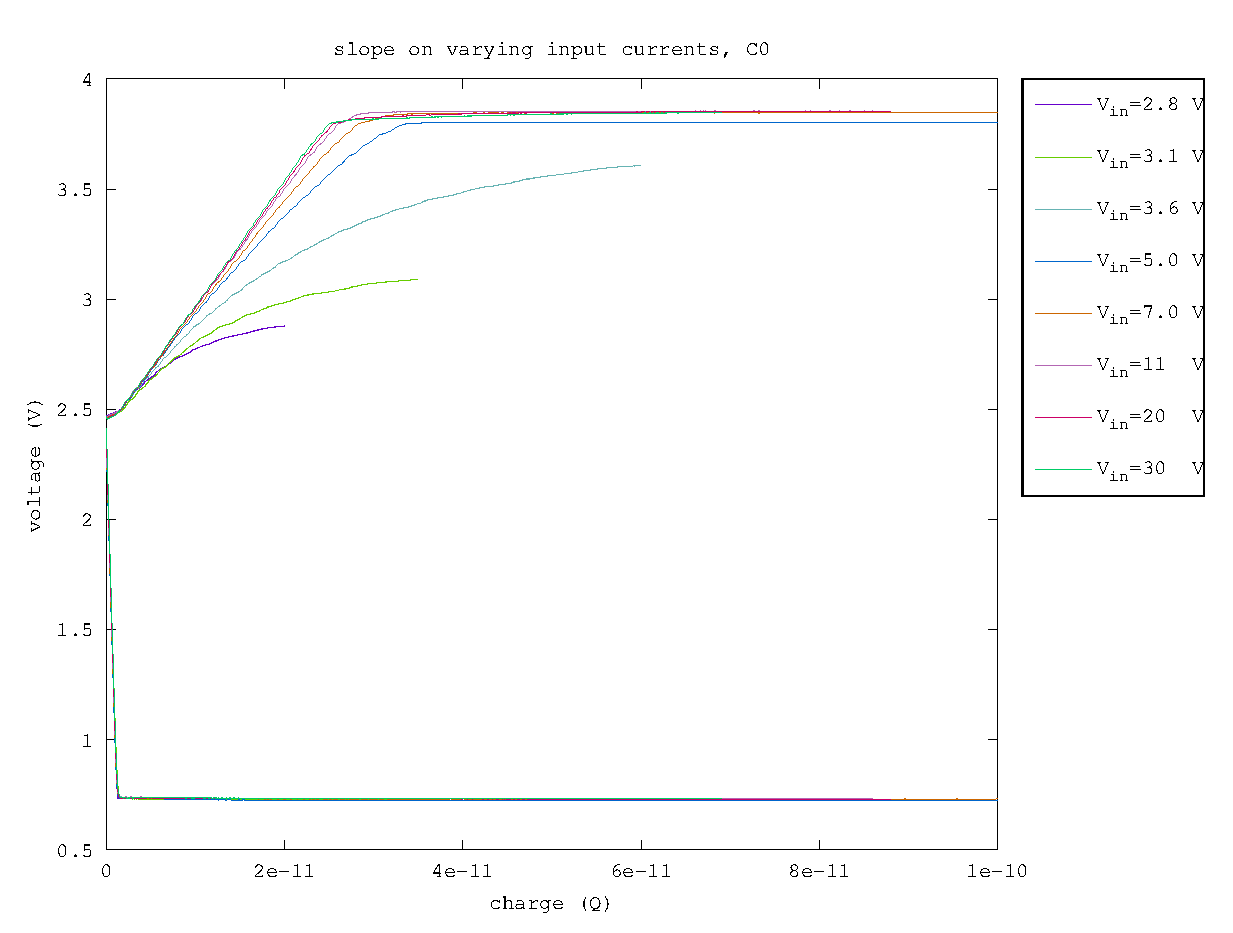
\includegraphics[width=\textwidth]{fig/vbo_charge_450fF.eps}
	    \caption[Network2]%
	    {$C=450\,fF$}    
	    \label{fig:vbo_charges_450fF}
	\end{subfigure}
	\hfill
	\begin{subfigure}[b]{0.475\textwidth}  
	    \centering 
	    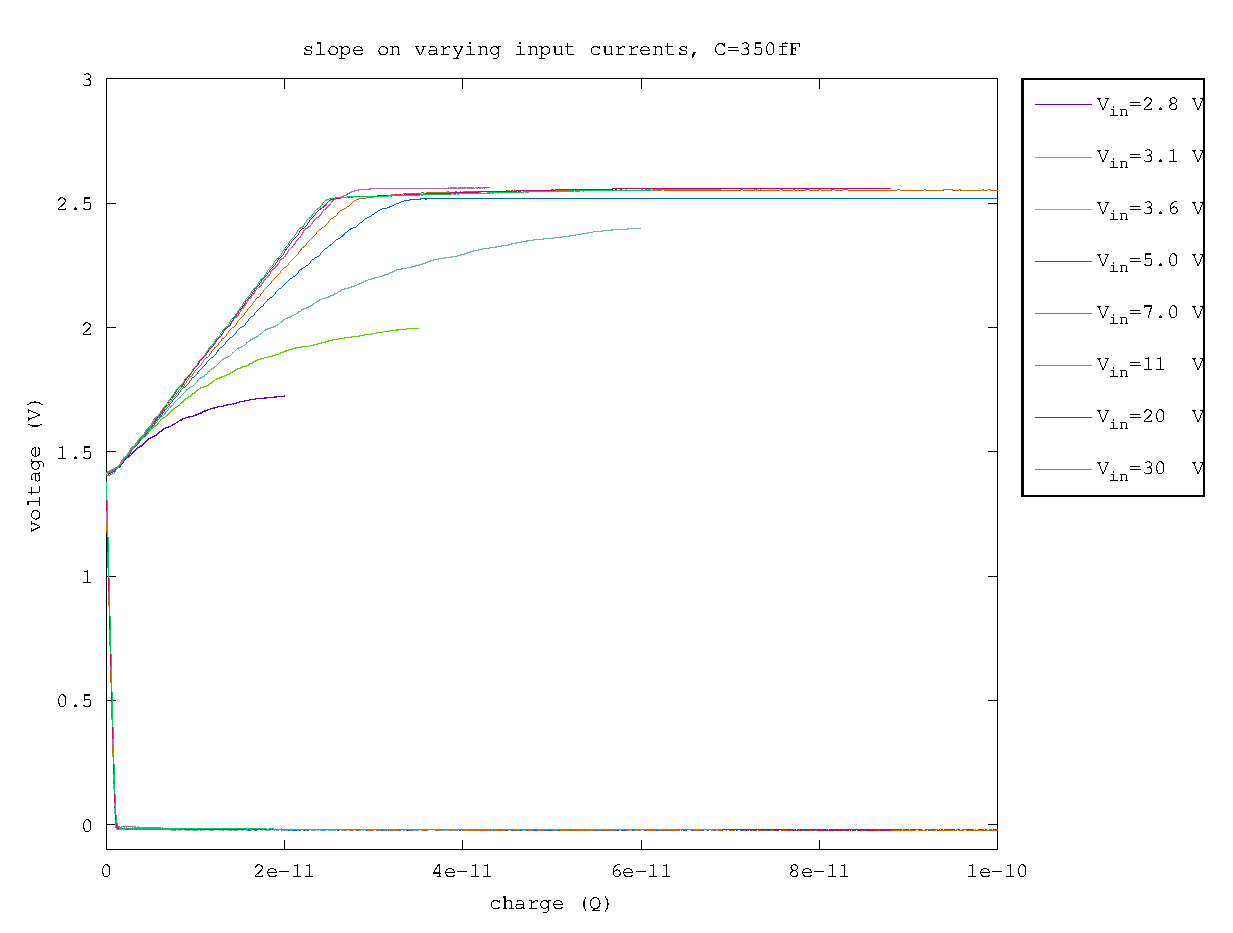
\includegraphics[width=\textwidth]{fig/vbo_charge_350fF.eps}
	    \caption[]%
	    {$C=350\,fF$}    
	    \label{fig:vbo_charges_350fF}
	\end{subfigure}
	\vskip\baselineskip
	\begin{subfigure}[b]{0.475\textwidth}   
	    \centering 
	    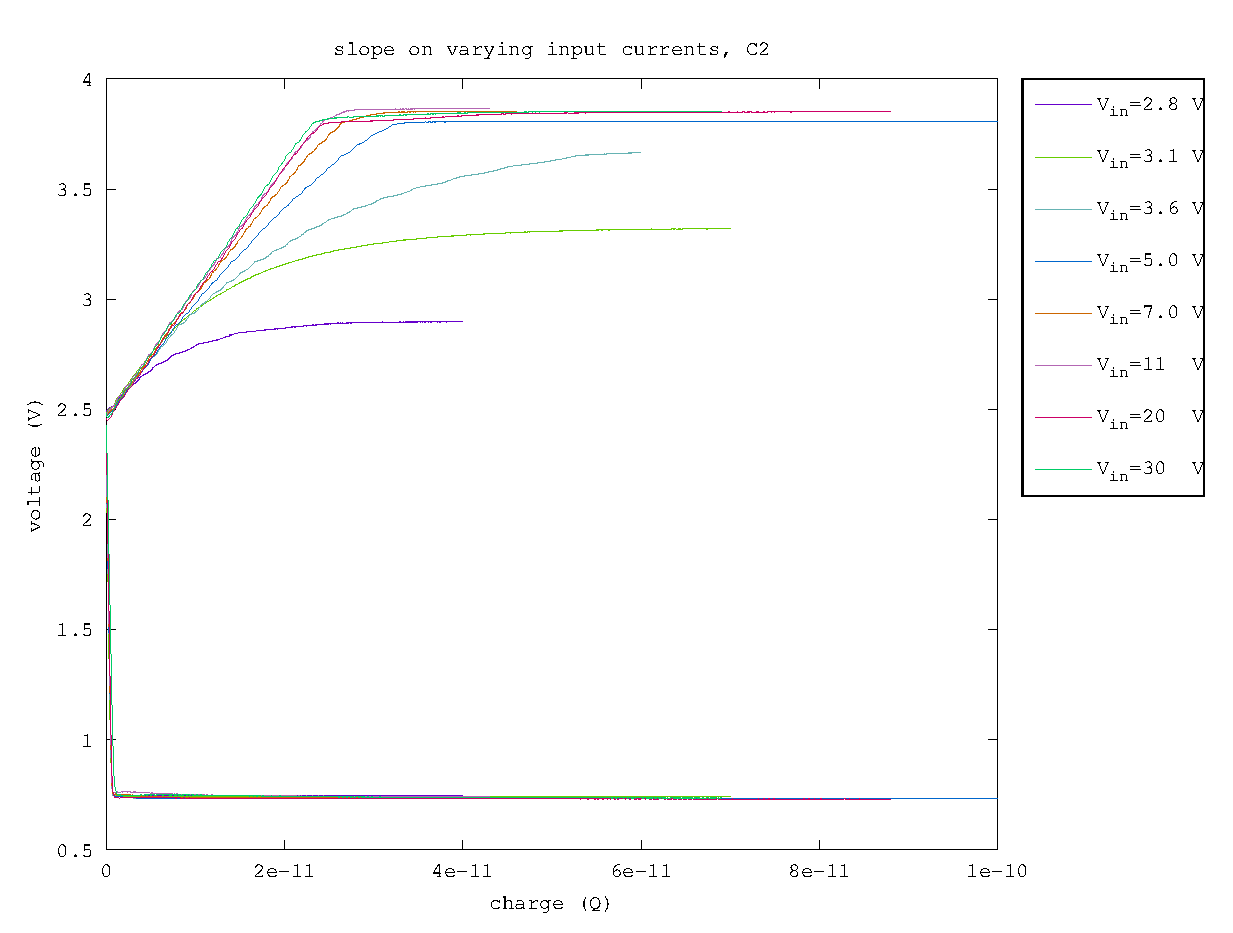
\includegraphics[width=\textwidth]{fig/vbo_charge_150fF.eps}
	    \caption[]%
	    {$C=150\,fF$}    
	    \label{fig:vbo_charges_150fF}
	\end{subfigure}
	\quad
	\begin{subfigure}[b]{0.475\textwidth}   
	    \centering 
	    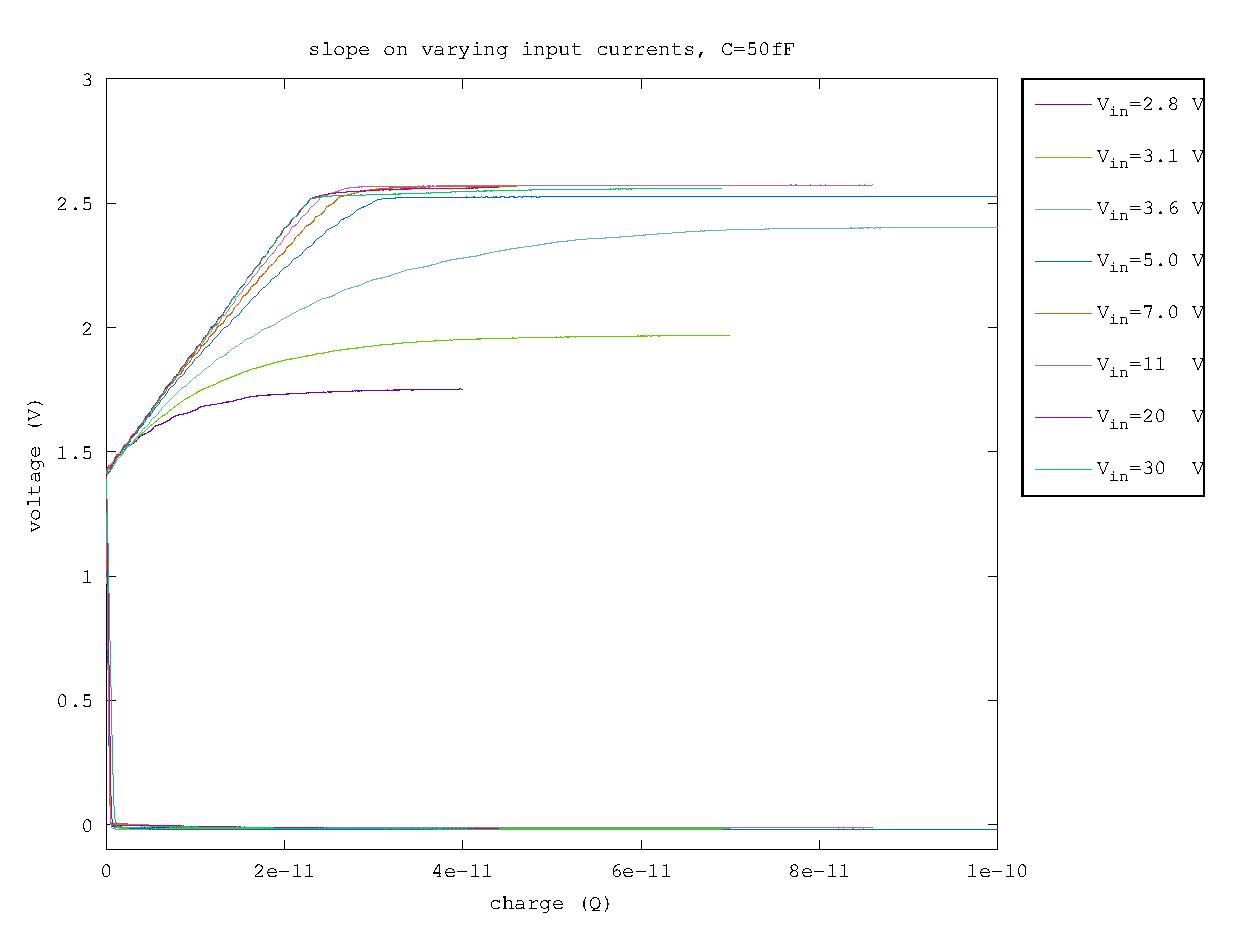
\includegraphics[width=\textwidth]{fig/vbo_charge_50fF.eps}
	    \caption[]%
	    {$C=50\,fF$}    
	    \label{fig:vbo_charges_50fF}
	\end{subfigure}
	\caption{This plot is showing charge versus voltage}
	\label{fig:vbo_charges}
\end{figure}

\Cref{fig:vbo_d_slopes} shows $\delta V/\delta Q$ for the VBO. The main observation one can make fromthese plots is that the behavior of VBO is almost entirely unaffected by the integration capacitance.


\begin{figure}[h]
	\centering
	\begin{subfigure}[b]{0.475\textwidth}
	    \centering
	    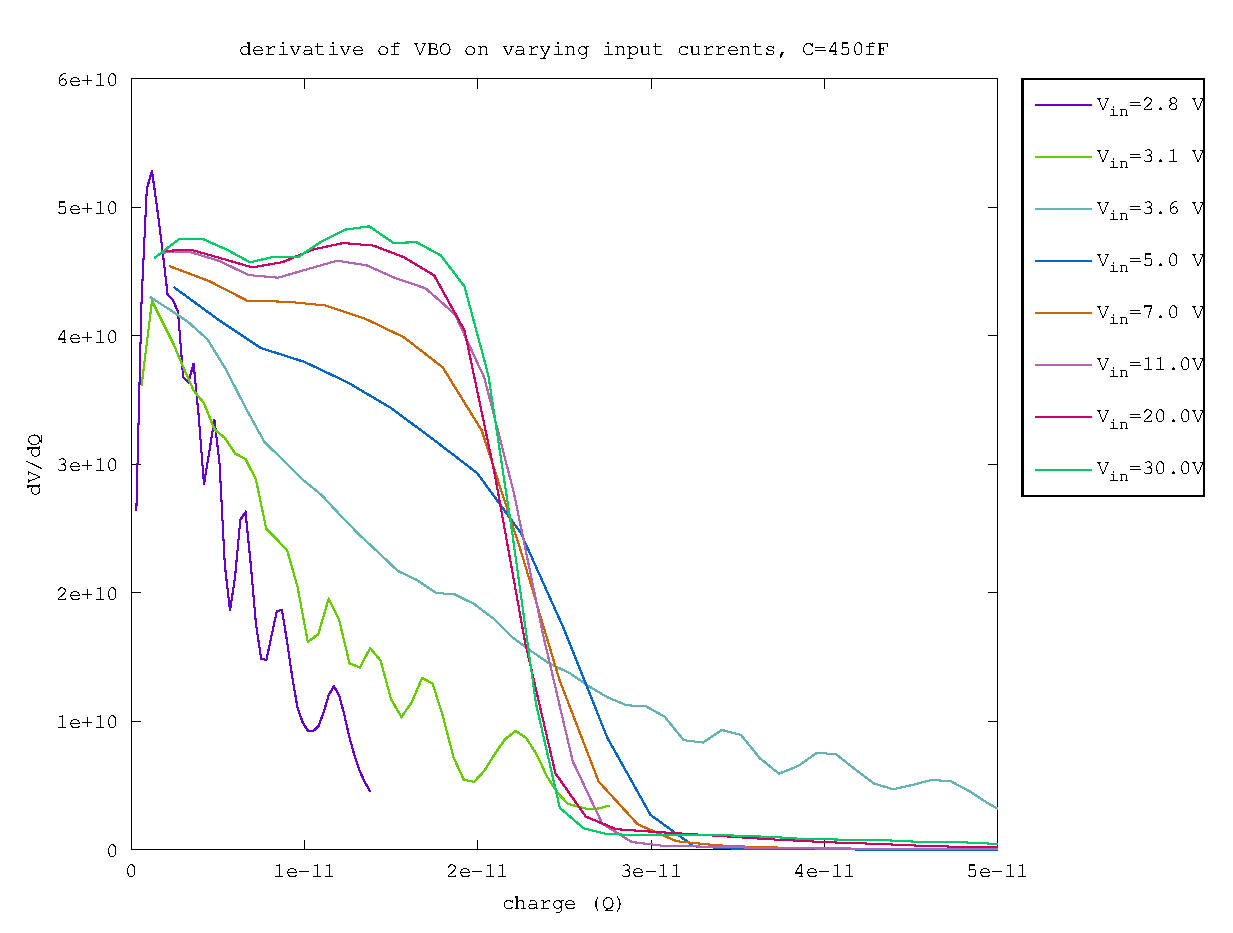
\includegraphics[width=\textwidth]{fig/vbo_d_slope_450fF.eps}
	    \caption[Network2]%
	    {$C=450\,fF$}    
	    \label{fig:vbo_d_slopes_450fF}
	\end{subfigure}
	\hfill
	\begin{subfigure}[b]{0.475\textwidth}  
	    \centering 
	    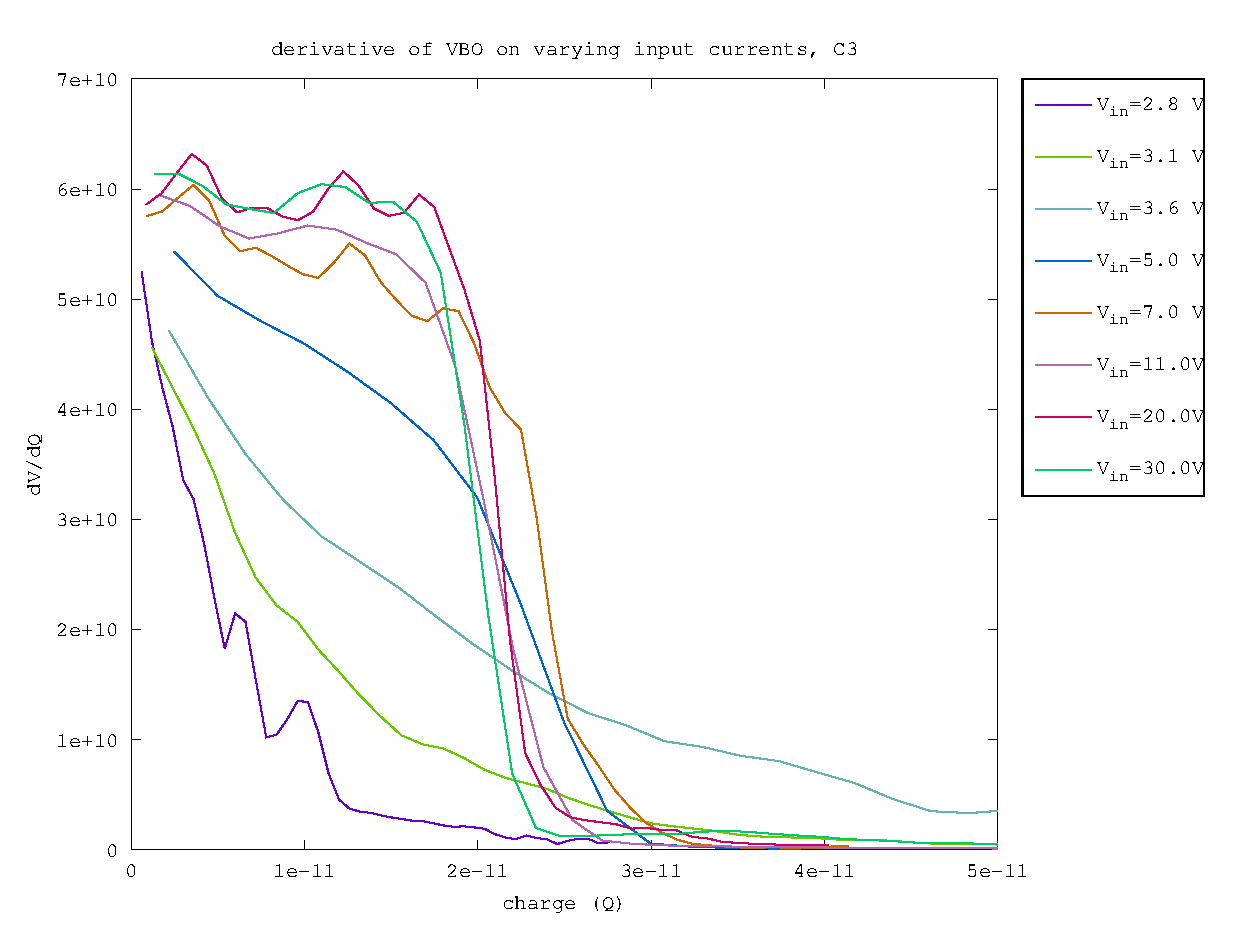
\includegraphics[width=\textwidth]{fig/vbo_d_slope_350fF.eps}
	    \caption[]%
	    {$C=350\,fF$}    
	    \label{fig:vbo_d_slopes_350fF}
	\end{subfigure}
	\vskip\baselineskip
	\begin{subfigure}[b]{0.475\textwidth}   
	    \centering 
	    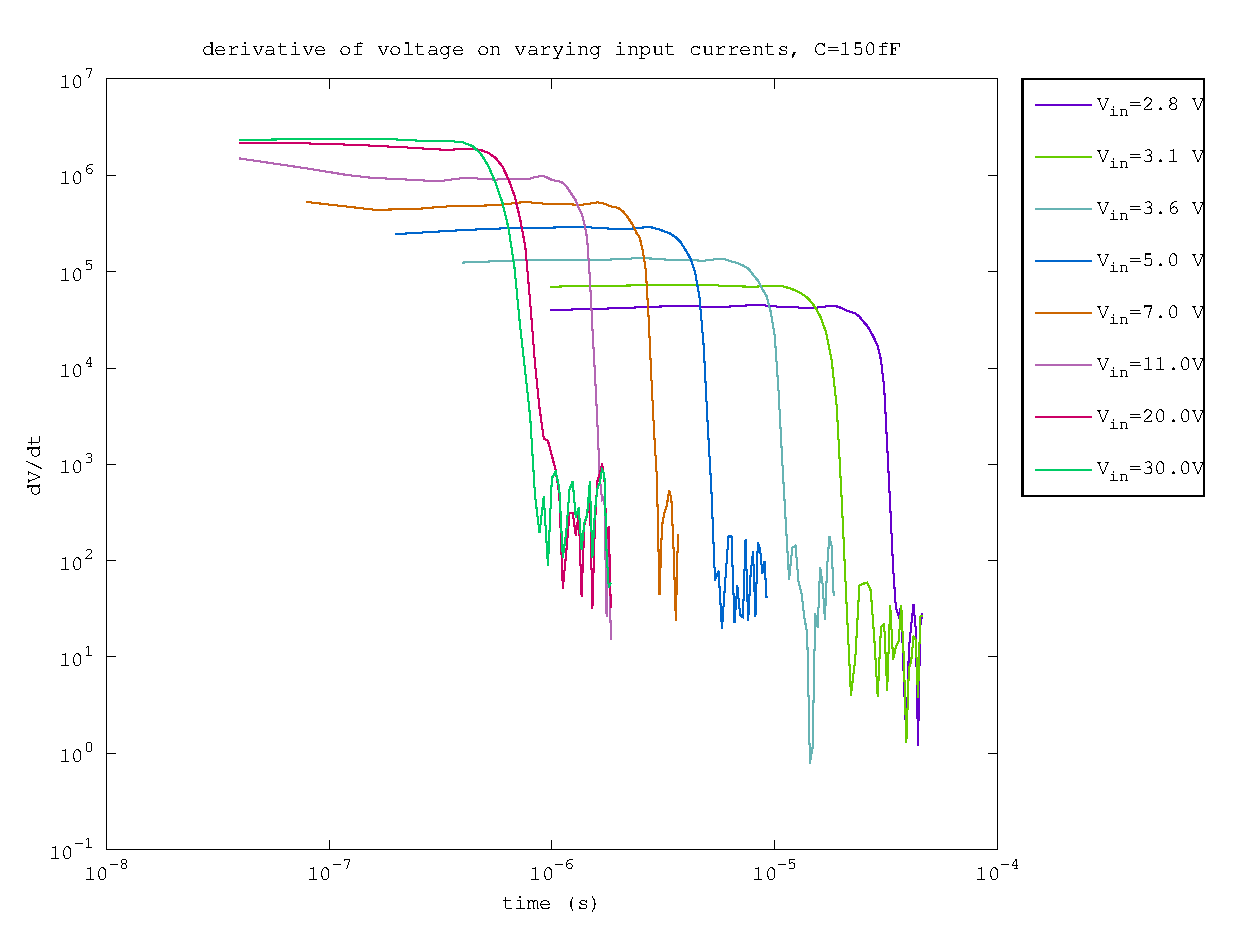
\includegraphics[width=\textwidth]{fig/vbo_d_slope_150fF.eps}
	    \caption[]%
	    {$C=150\,fF$}    
	    \label{fig:vbo_d_slopes_150fF}
	\end{subfigure}
	\quad
	\begin{subfigure}[b]{0.475\textwidth}   
	    \centering 
	    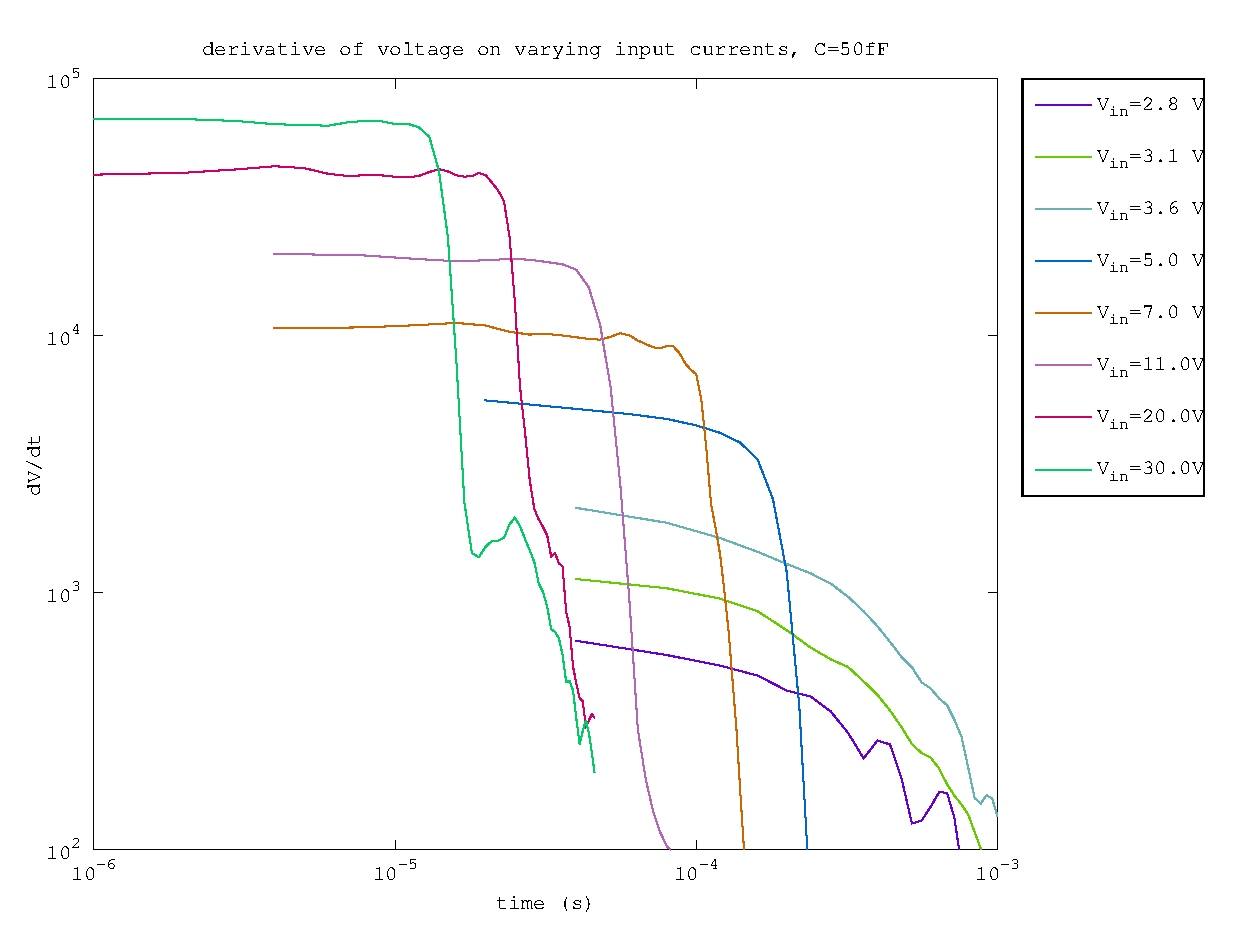
\includegraphics[width=\textwidth]{fig/vbo_d_slope_50fF.eps}
	    \caption[]%
	    {$C=50\,fF$}    
	    \label{fig:vbo_d_slopes_50fF}
	\end{subfigure}
	\caption{The plot shows dv/dt against time of the vbo.}
	\label{fig:vbo_d_slopes}
\end{figure}


\Cref{fig:vbo_e_vs_m} shows the $\delta V/\delta t$ against input voltage for VBO across all capacitances. For large voltages seem to behave in a noemal linear fashon. The startup shows a scene that looks as if the $450\,fF$ and $350\,fF$ setup behave identical, and that the $150\,fF$ and $50\,fF$ setup behave identical. This might be due to the lack of measurement points, but is worth investigating further.



\begin{figure}[h]
	    \centering
	    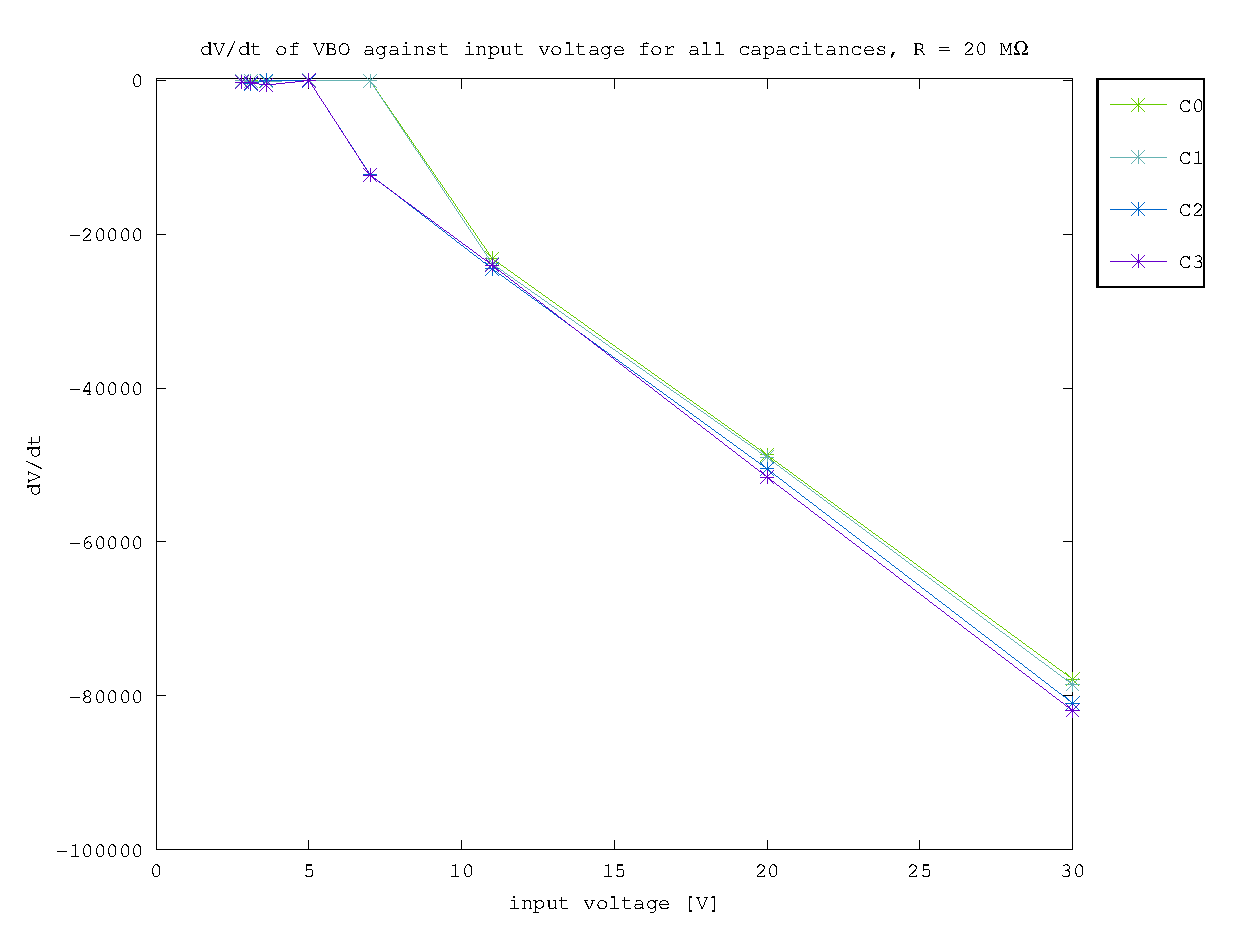
\includegraphics[width=\textwidth]{fig/vbo_vin_vs_time_sat.eps}
	    \caption[]%
	    {dV/dt of VBO against input voltage for all four capacitances. The x indicate the measurements.}    
	    \label{fig:vbo_e_vs_m}	
\end{figure}


\Cref{fig:vg_vs_vbo} shows the relationship between $V_g$ and the voltage limit posed by the high voltage transistor at the input. 

\begin{figure}[h]
	    \centering
	    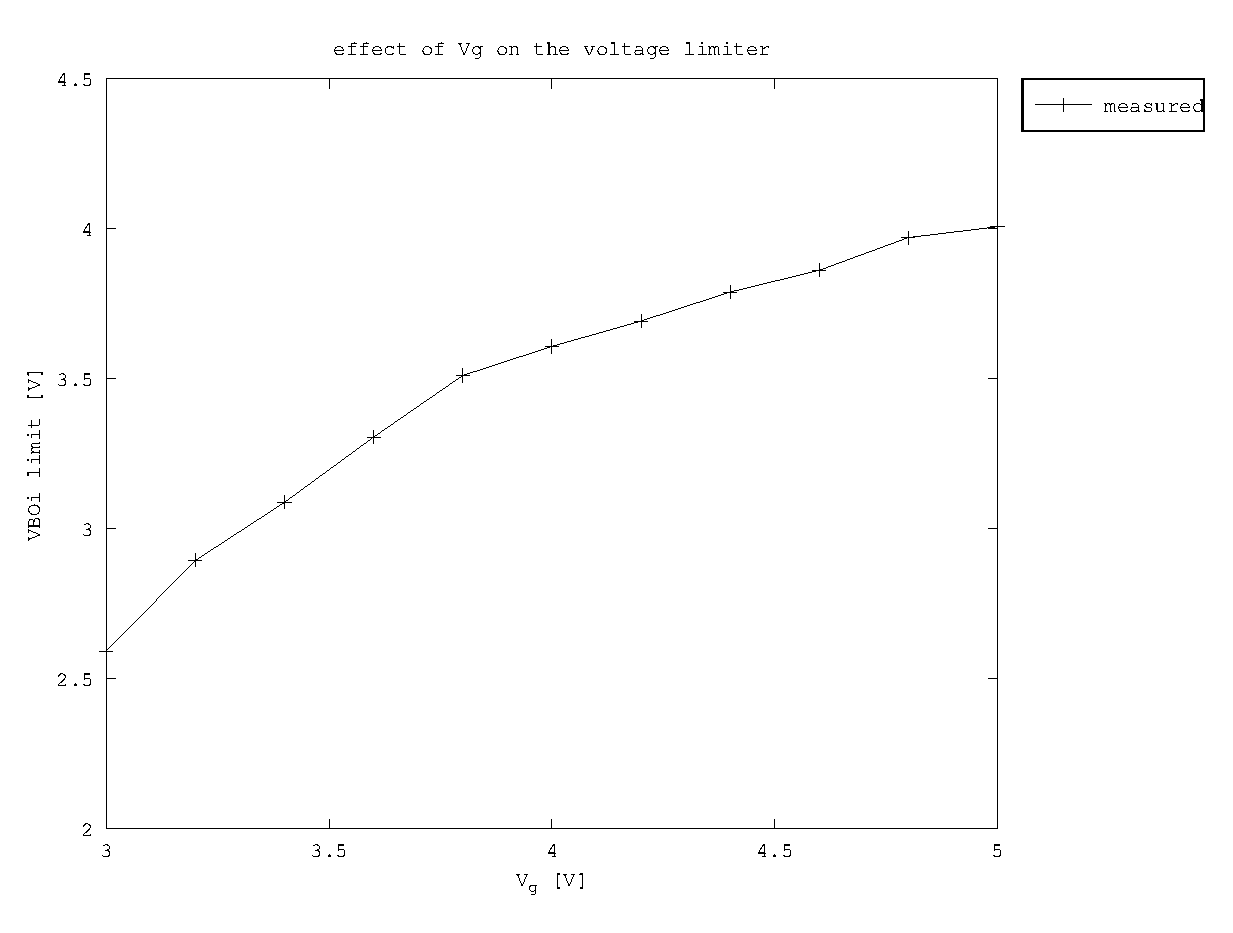
\includegraphics[width=\textwidth]{fig/vg_vs_vbo.eps}
	    \caption[]%
	    {voltage limit as a function of Vg}    
	    \label{fig:vg_vs_vbo}	
\end{figure}





\clearpage



\section{Characterization of GaN sensors}

\begin{figure}[h]
	\centering
	\begin{subfigure}[b]{0.475\textwidth}
	    \centering
	    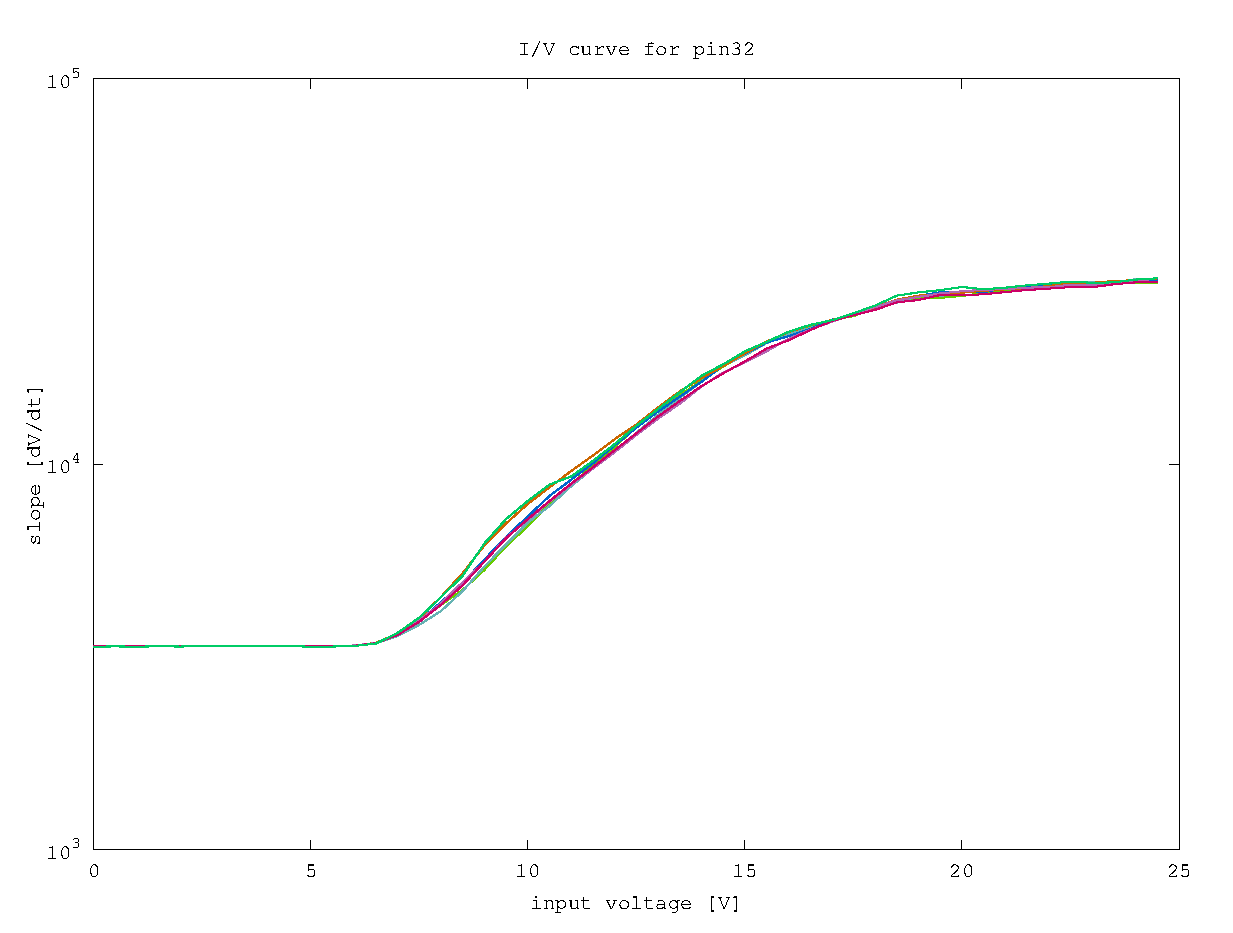
\includegraphics[width=\textwidth]{fig/pin32_slope_0-25V.eps}
	    \caption[Network2]%
	    {I/V characteristics}    
	    \label{fig:pin32_slope}
	\end{subfigure}
	\hfill
	\begin{subfigure}[b]{0.475\textwidth}  
	    \centering 
	    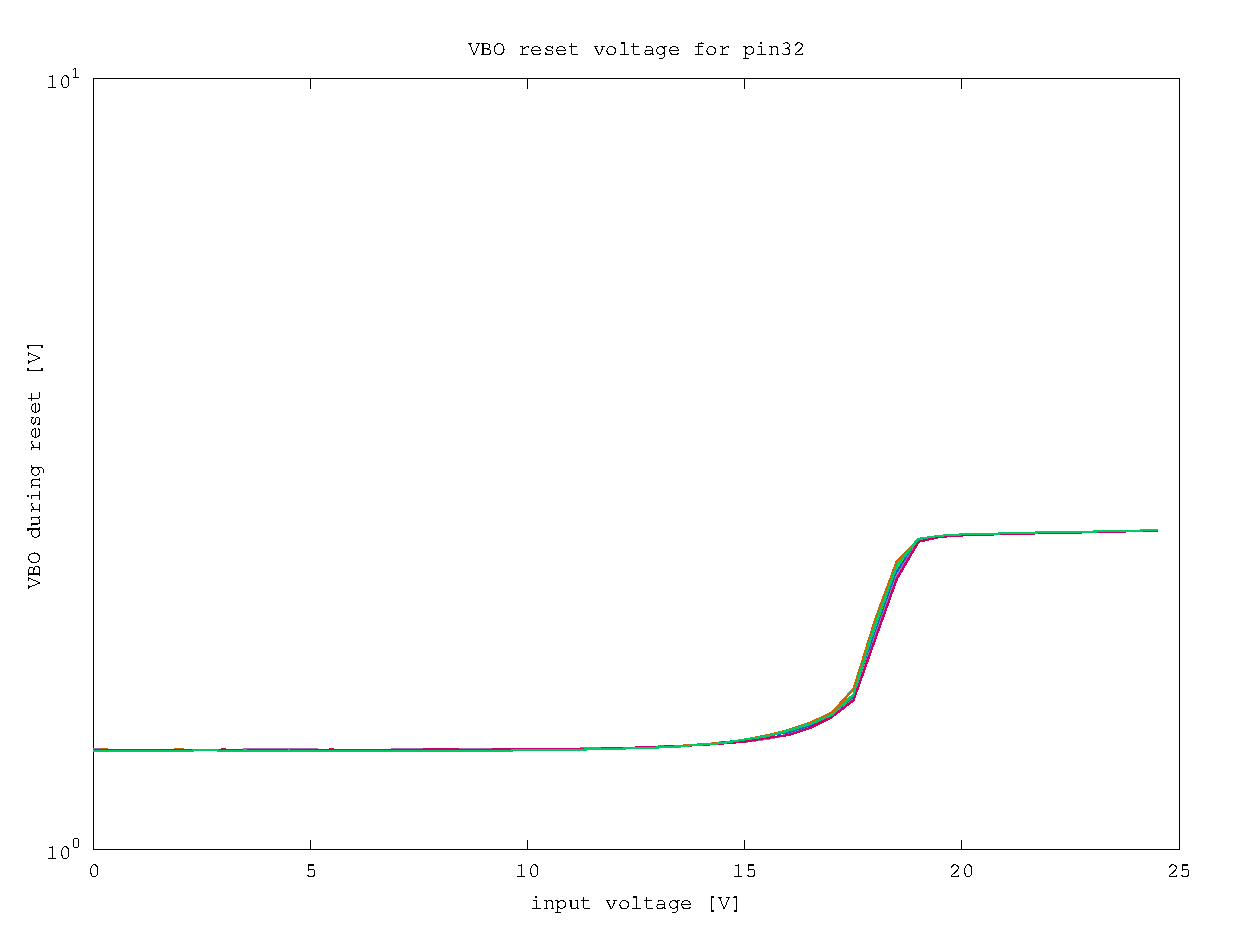
\includegraphics[width=\textwidth]{fig/pin32_reset_0-25V.eps}
	    \caption[]%
	    {reset value for VBO}    
	    \label{fig:pin32_reset}
	\end{subfigure}
	\caption{The slope and reset values for the VBO of pin32 repeated multiple times to test variance across measurements}
	\label{fig:pin32}
\end{figure}

\begin{figure}[h]
	\centering
	\begin{subfigure}[b]{0.475\textwidth}
	    \centering
	    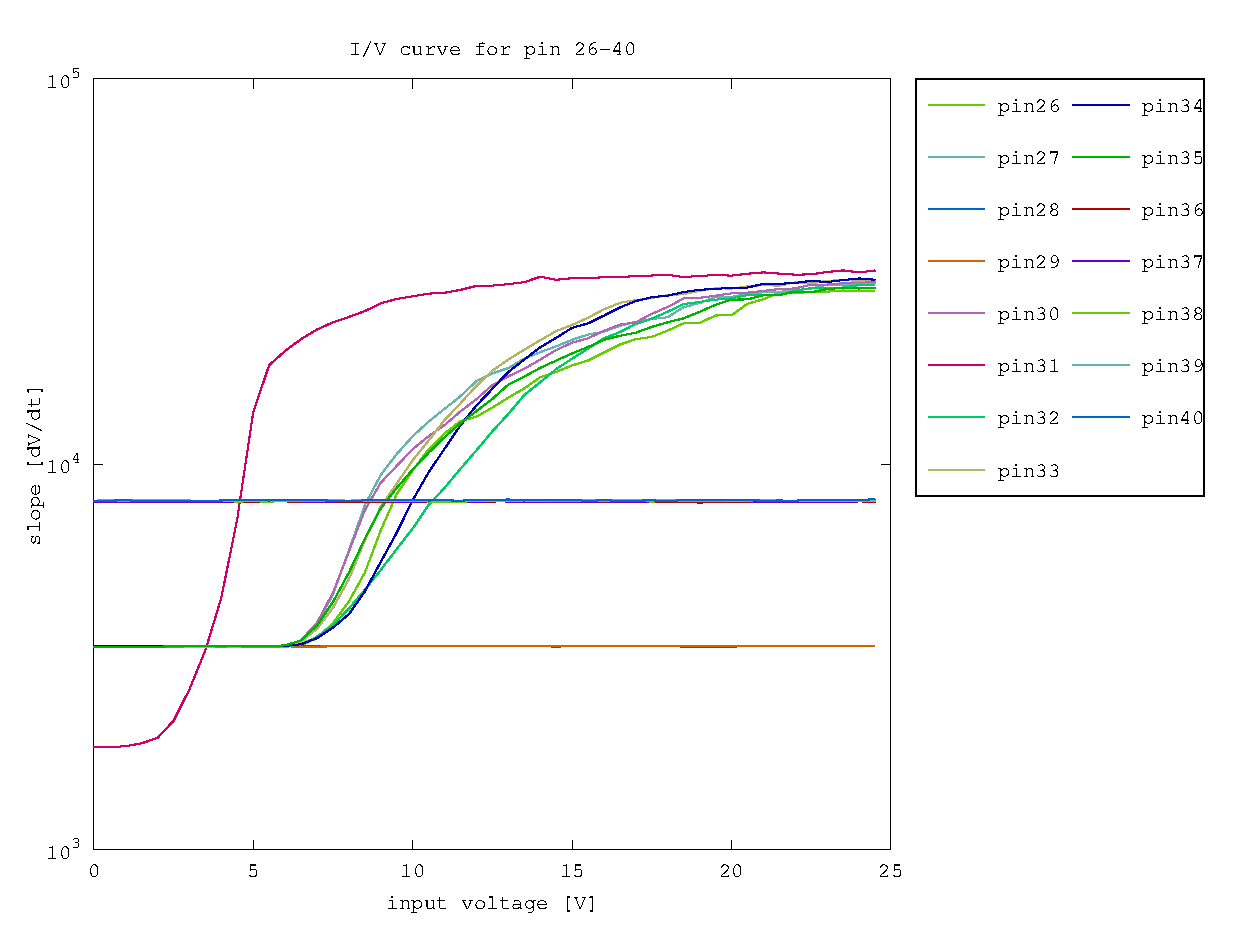
\includegraphics[width=\textwidth]{fig/pin26-40_slope_0-25V.eps}
	    \caption[Network2]%
	    {I/V characteristics}    
	    \label{fig:pin26-40_slope}
	\end{subfigure}
	\hfill
	\begin{subfigure}[b]{0.475\textwidth}  
	    \centering 
	    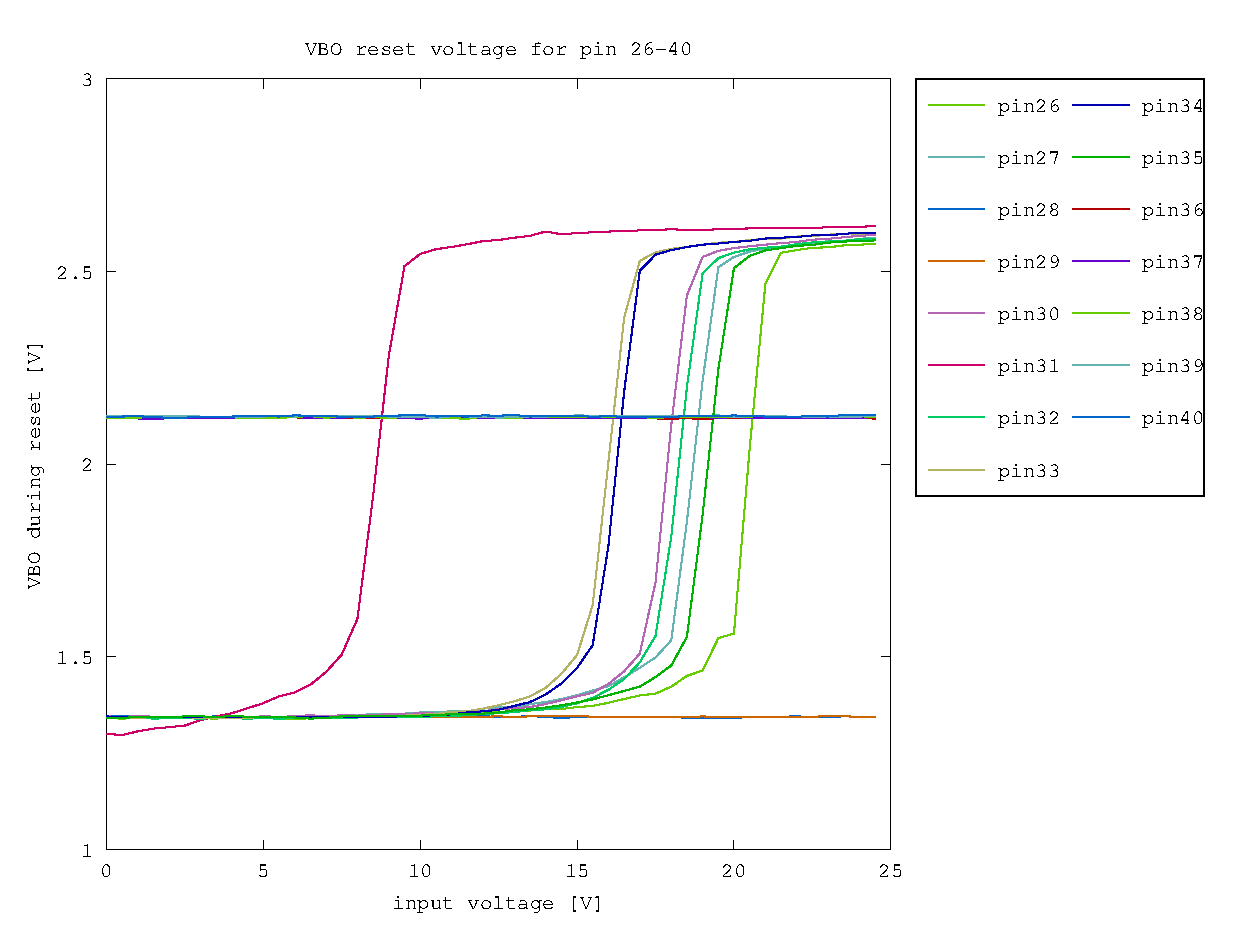
\includegraphics[width=\textwidth]{fig/pin26-40_reset_0-25V.eps}
	    \caption[]%
	    {reset value for VBO}    
	    \label{fig:pin26-40_reset}
	\end{subfigure}
	\caption{The slope and reset values for the VBO of pin26-40}
	\label{fig:pin32}
\end{figure}


\begin{figure}[h]
	\centering
	\begin{subfigure}[b]{0.475\textwidth}
	    \centering
	    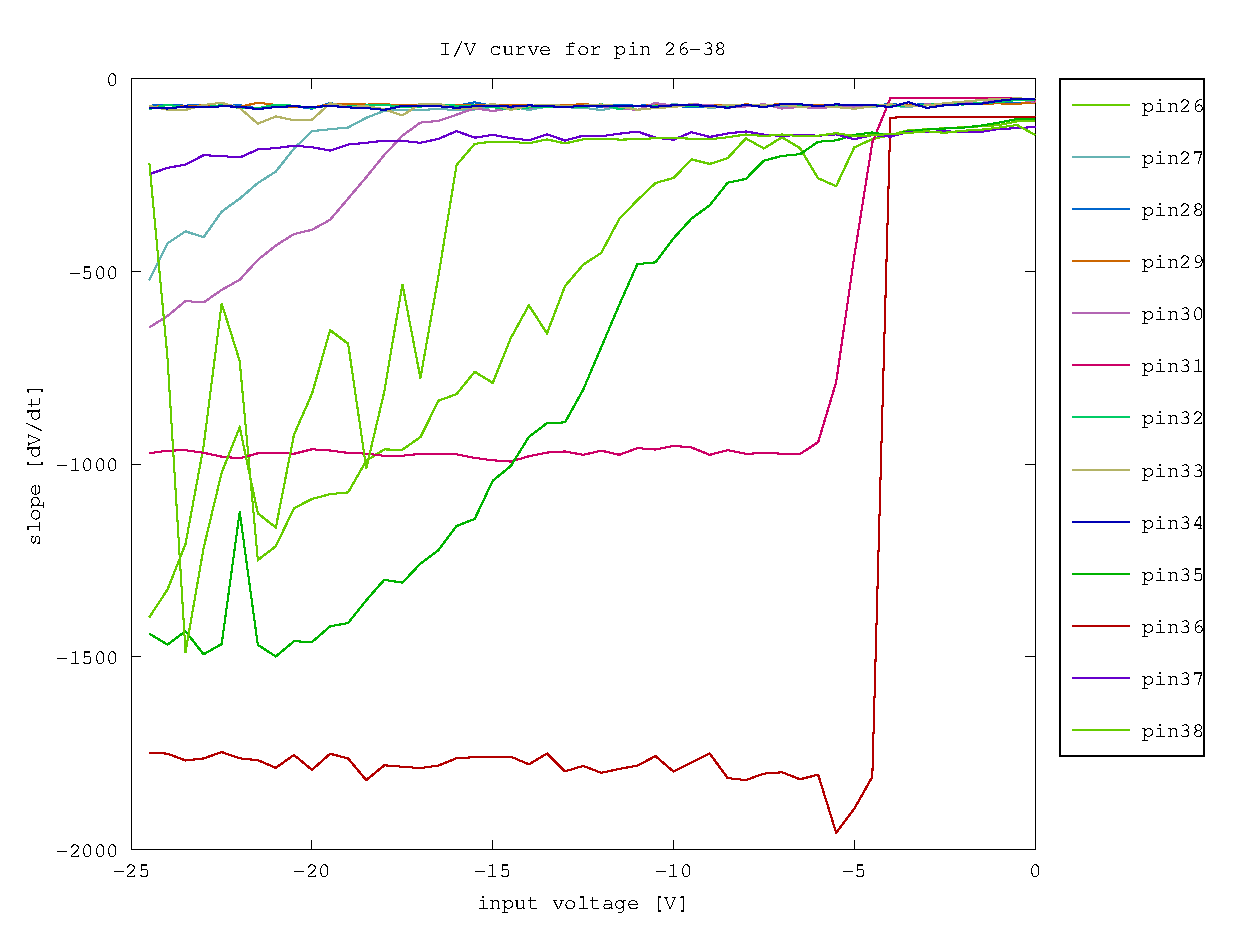
\includegraphics[width=\textwidth]{fig/pin26-38_slope_-25-0V.eps}
	    \caption[Network2]%
	    {I/V characteristics}    
	    \label{fig:pin26-40_slope}
	\end{subfigure}
	\hfill
	\begin{subfigure}[b]{0.475\textwidth}  
	    \centering 
	    \includegraphics[width=\textwidth]{fig/pin26-38_reset_-25-0V.eps}
	    \caption[]%
	    {reset value for VBO}    
	    \label{fig:pin26-40_reset}
	\end{subfigure}
	\caption{The slope and reset values for the OUT of pin26-38}
	\label{fig:pin32}
\end{figure}


\begin{figure}[h]
	\centering
	\begin{subfigure}[b]{0.475\textwidth}
	    \centering
	    \includegraphics[width=\textwidth]{fig/pin24_slope_-25-0V.eps}
	    \caption[Network2]%
	    {I/V characteristics}    
	    \label{fig:pin24_slope}
	\end{subfigure}
	\hfill
	\begin{subfigure}[b]{0.475\textwidth}  
	    \centering 
	    \includegraphics[width=\textwidth]{fig/pin24_reset_-25-0V.eps}
	    \caption[]%
	    {reset value for VBO}    
	    \label{fig:pin24_reset}
	\end{subfigure}
	\caption{The slope and reset values for the OUT of pin24}
	\label{fig:pin32}
\end{figure}


\begin{figure}[h]
	    \centering
	    \includegraphics[width=\textwidth]{fig/pin22-30_slope_-25-0V.eps}
	    \caption[]%
	    {voltage limit as a function of Vg}    
	    \label{fig:vg_vs_vbo}	
\end{figure}


\end{document}



